\documentclass[a4paper,14pt]{extarticle}

\usepackage[T2A]{fontenc}
\usepackage[utf8]{inputenc}
\usepackage[english,russian]{babel}

\usepackage{amsthm}
\usepackage{amssymb}
\usepackage{amsmath}
\usepackage{bm}
\usepackage{booktabs}
\usepackage{caption}
\usepackage{graphicx}
\usepackage{float}
\usepackage{indentfirst}
\usepackage{longtable}
\usepackage{mathtools}
\usepackage{multirow}
\usepackage{rotating}
\usepackage{subfig}
\usepackage{tabularx}
\usepackage{url}
\usepackage{xcolor}
\usepackage{setspace}

\usepackage{geometry}
\geometry{
    left=3.0cm,
    right=1.5cm,
    top=2.0cm,
    bottom=2.0cm
}
\onehalfspacing
\setlength{\parindent}{1.25cm}
\emergencystretch=3em

\graphicspath{{thesis_assets/figures/}{thesis_assets/results/}}

\DeclareMathOperator*{\argmax}{arg\,max}
\DeclareMathOperator*{\argmin}{arg\,min}
\DeclareMathOperator{\diam}{diam}
\DeclareMathOperator{\diag}{diag}

\newtheorem{theorem}{Теорема}
\newtheorem{lemma}[theorem]{Лемма}
\newtheorem{definition}{Определение}[section]
\newtheorem{proposition}[theorem]{Утверждение}
\newtheorem{corollary}[theorem]{Следствие}
\newtheorem{assumption}[theorem]{Предположение}

\numberwithin{equation}{section}

\newcommand*{\No}{No.}
\newcommand{\R}{\mathbb{R}}
\newcommand{\E}{\mathbb{E}}
\newcommand{\cX}{\mathcal{X}}
\newcommand{\cC}{\mathcal{C}}
\newcommand{\cF}{\mathcal{F}}
\newcommand{\cE}{\mathcal{E}}
\newcommand{\cV}{\mathcal{V}}
\newcommand{\cP}{\mathcal{P}}
\newcommand{\cI}{\mathcal{I}}
\newcommand{\cD}{\mathcal{D}}
\newcommand{\norm}[1]{\left\|#1\right\|}
\newcommand{\inner}[2]{\left\langle #1, #2 \right\rangle}
\newcommand{\Sum}{\sum\limits}
\newcommand{\Max}{\max\limits}
\newcommand{\Min}{\min\limits}
\newcommand{\cG}{\mathcal{G}}
\newcommand{\cO}{\mathcal{O}}
\newcommand{\br}[1]{\left[#1\right]}
\newcommand{\cbr}[1]{\left(#1\right)}
\newcommand{\sqn}[1]{\norm{#1}_2^2}

\floatstyle{ruled}
\newfloat{algorithm}{H}{loa}
\floatname{algorithm}{Алгоритм}
\newenvironment{algorithmic}[1][]
{\begin{minipage}{0.96\textwidth}\small\setlength{\parskip}{3pt}}
{\end{minipage}}
\newcommand{\STATE}{\par\noindent}
\newcommand{\REQUIRE}{\STATE\textbf{Вход:} }
\newcommand{\ENSURE}{\STATE\textbf{Выход:} }
\newcommand{\FOR}[1]{\STATE\textbf{для } #1 \textbf{ выполнить}}
\newcommand{\FORALL}[1]{\STATE\textbf{для всех } #1 \textbf{ выполнить}}
\newcommand{\ENDFOR}{\STATE\textbf{конец цикла}}
\newcommand{\IF}[1]{\STATE\textbf{если } #1 \textbf{, то}}
\newcommand{\ENDIF}{\STATE\textbf{конец условия}}
\newcommand{\REPEAT}{\STATE\textbf{повторять}}
\newcommand{\UNTIL}[1]{\STATE\textbf{пока не выполнено } #1}
\newcommand{\COMMENT}[1]{\hfill{\footnotesize // #1}}
\newcommand{\State}{\STATE}
\newcommand{\Require}{\REQUIRE}
\newcommand{\Ensure}{\ENSURE}
\newcommand{\For}[1]{\FOR{#1}}
\newcommand{\ForAll}[1]{\FORALL{#1}}
\newcommand{\EndFor}{\ENDFOR}
\newcommand{\If}[1]{\IF{#1}}
\newcommand{\EndIf}{\ENDIF}
\newcommand{\Comment}[1]{\COMMENT{#1}}
\newcommand{\Statex}{\STATE}

% Project metadata.
\newcommand{\UniversityName}{Министерство науки и высшего образования Российской Федерации\\
Федеральное государственное автономное образовательное учреждение высшего образования\\
<<Московский физико-технический институт (национальный исследовательский институт)>>}
\newcommand{\FacultyName}{Факультет управления и прикладной математики}
\newcommand{\DepartmentName}{Кафедра <<Интеллектуальные системы>>}
\newcommand{\ProgramName}{09.04.01 <<Информатика и вычислительная техника>>}
\newcommand{\ThesisTitle}{Приложения алгоритма Франк-Вульфа к задачам машинного обучения}
\newcommand{\AuthorGroup}{}
\newcommand{\AuthorName}{Игнашин Игорь Николаевич}
\newcommand{\SupervisorDegree}{доктор физико-математических наук}
\newcommand{\SupervisorName}{Грабовой Андрей Олегович}
\newcommand{\CityYear}{Москва 2026}

\begin{document}

\begin{titlepage}
    \begin{center}
        \UniversityName\\
        \FacultyName\\
        \DepartmentName
    \end{center}

    \vspace{2cm}

    \begin{center}
        {\Large \bfseries \ThesisTitle}
    \end{center}

    \begin{center}
        ~\\[-28pt]
        Выпускная квалификационная работа\\
        (магистерская диссертация)
    \end{center}

    \vspace{0.5cm}

    \begin{center}
        \textbf{Направление подготовки:}~\ProgramName
    \end{center}

    \begin{flushright}
        \begin{tabular}{l}
            \textbf{Выполнил:}\\
            магистрант\\
            \AuthorName\\
            \underline{\hspace{7cm}}\\[-10pt]
            \begin{scriptsize}
                \hspace{3.5cm}(подпись обучающегося)
            \end{scriptsize}\\[15pt]
            \textbf{Научный руководитель:}\\
            \SupervisorDegree\\
            \SupervisorName\\
            \underline{\hspace{7cm}}\\[-10pt]
            \begin{scriptsize}
                \hspace{3.1cm}(подпись научного руководителя)
            \end{scriptsize}
        \end{tabular}
    \end{flushright}

    \vfill

    \begin{center}
        \CityYear
    \end{center}
\end{titlepage}


% Нумерация обычно начинается со второй страницы.
\setcounter{page}{2}

\newpage

\begin{abstract}
Работа посвящена приложениям алгоритма Frank--Wolfe к задачам машинного обучения и смежным задачам крупномасштабной выпуклой оптимизации.
Цель работы состоит в развитии проекционно-свободных модификаций Frank--Wolfe, уменьшающих вычислительную стоимость итерации без потери базовых гарантий сходимости.
Для достижения этой цели рассматриваются методы с памятью о предыдущих направлениях, перенос CFW и NFW на гладкие задачи машинного обучения, стохастический блочно-координатный SOFW для транспортных сетей и децентрализованный блочно-координатный DBCFW.
Получены оценки сходимости для CFW, SOFW и DBCFW, описаны специальные случаи этих методов и проведены эксперименты для логистической регрессии и задач распределения транспортных потоков.
Результаты работы могут использоваться при выборе модификации Frank--Wolfe под конкретное вычислительное ограничение: стоимость линейного оракула, выбор направления или распределенный характер данных.

\smallskip
\textit{Ключевые слова}: Frank--Wolfe; условный градиент; машинное обучение; выпуклая оптимизация; моментум по направлениям; сопряженные направления; SOFW; стохастический LMO; блочно-координатная оптимизация; распределенная оптимизация.
\end{abstract}


\newpage
\setcounter{tocdepth}{2}
\tableofcontents

\newpage

\section*{Обозначения и сокращения}
\addcontentsline{toc}{section}{Обозначения и сокращения}

В работе используется единая система обозначений для рассматриваемых методов.
Часть обозначений относится к транспортной постановке, часть -- к общей выпуклой
и распределенной оптимизации.
Ниже приведено согласование обозначений, которое используется в дальнейшем тексте.

\begin{description}
    \item[$\cX$, $D$] допустимое множество; в транспортной задаче обычно множество путевых потоков, в ML-задаче множество параметров модели.
    \item[$D_1\times\dots\times D_n$] декартова блочная структура допустимого множества.
    \item[$x$] переменная оптимизации в общей задаче и в задачах машинного обучения.
    \item[$f$] поток по ребрам транспортной сети; также $f(x)$ обозначает целевую функцию в общей оптимизации, если это не конфликтует с контекстом.
    \item[$\Psi(f)$] потенциал Бекмана в задаче равновесного распределения транспортных потоков.
    \item[$\tau(f)$] вектор времен движения по ребрам; равен $\nabla\Psi(f)$.
    \item[$\Theta$] матрица принадлежности ребер путям, переводящая путевые потоки в потоки по ребрам.
    \item[$OD$] множество пар источник--сток.
    \item[$\cP_{ij}$] множество путей между источником $i$ и стоком $j$.
    \item[$d_{ij}$] спрос между источником $i$ и стоком $j$.
    \item[$s_k^{FW}$] решение линейного оракула Frank--Wolfe на итерации $k$.
    \item[$d_k$] направление шага; в транспортных главах не смешивается со спросом $d_{ij}$, потому что индекс и контекст различают эти величины.
    \item[$\gamma_k$] длина шага FW.
    \item[$g_k$] зазор Frank--Wolfe.
    \item[$H_k$] гессиан целевой функции в текущей точке.
    \item[$N$] в главах о NFW -- число прошлых направлений; в главе о DBCFW -- число агентов, если явно указан распределенный контекст.
    \item[$B$] размер батча блоков в DBCFW.
    \item[$W_t$] матрица смешивания коммуникационного графа.
    \item[$x_t^i$] локальная точка агента $i$ на итерации $t$.
    \item[$g_t^i$] локальная оценка градиента в градиентном отслеживании.
    \item[$x_{\mathrm{avg},t}$] средняя точка по агентам.
\end{description}

\subsection*{Сокращения}
\addcontentsline{toc}{subsection}{Сокращения}

\begin{description}
    \item[FW] Frank--Wolfe, метод условного градиента.
    \item[CFW] Conjugate Frank--Wolfe.
    \item[BFW] Bi-conjugate Frank--Wolfe.
    \item[NFW] N-conjugate Frank--Wolfe.
    \item[FFW] Fukushima Frank--Wolfe.
    \item[WFFW] Weighted Fukushima Frank--Wolfe.
    \item[BCFW] Block-Coordinate Frank--Wolfe, блочно-координатный Frank--Wolfe.
    \item[SOFW] Stochastic Origin Frank--Wolfe.
    \item[DFW] Decentralized Frank--Wolfe.
    \item[DBCFW] Decentralized Block-Coordinate Frank--Wolfe.
    \item[LMO] linear minimization oracle, линейный оракул.
    \item[BPR] Bureau of Public Roads travel time function.
    \item[OD] origin--destination pair, пара источник--сток.
\end{description}

\subsection*{Линия развития методов}

Рассматриваемая линия методов может быть интерпретирована как последовательное расширение
проекционно-свободной оптимизации по трем исследовательским осям: геометрия направления,
стоимость линейного оракула и распределенная информационная структура.
Первое направление связано с улучшением геометрии шага Frank--Wolfe.
В транспортной задаче это приводит к методам CFW, BFW, NFW, FFW и WFFW, которые используют
память о предыдущих направлениях для уменьшения зигзагообразного поведения траектории.

Второе направление состоит в адаптации сопряженных FW-методов к задачам машинного обучения.
Главная трудность состоит в стоимости вычисления и хранения гессиана, а также в стоимости
точных произведений гессиана на направления.
Поэтому информация о кривизне приближается конечными разностями градиентов.
Так сохраняется идея сопряженности, но алгоритм остается практически применимым.

Третье направление исследует другой вычислительный предел FW -- стоимость полного линейного
оракула.
В крупной транспортной сети полный оракул требует решать задачи кратчайших путей для всех
источников на каждой итерации.
SOFW заменяет полный оракул случайным блочным оракулом и тем самым связывает транспортный
Frank--Wolfe с теорией стохастических блочно-координатных методов.

Четвертое направление обобщает блочную стохастичность на распределенную оптимизацию.
DBCFW соединяет локальные функции агентов, консенсус через матрицу смешивания, отслеживание
градиента и блочный линейный оракул.
Тем самым случайный выбор блоков становится частью децентрализованной схемы условного
градиента.

\newpage

\section{Введение}

Алгоритм Frank--Wolfe, также известный как метод условного градиента, был предложен для задач квадратичного программирования и стал одним из базовых проекционно-свободных методов выпуклой оптимизации~\cite{frank1956algorithm}.
В отличие от проекционных градиентных методов, на каждой итерации он решает линейную задачу минимизации на допустимом множестве.
Это делает метод особенно удобным для задач, в которых линейный оракул существенно дешевле евклидовой проекции: оптимизация на симплексах, транспортных политопах, ядерных шарах, множествах с ограничением на $l_1$-норму и других структурированных областях~\cite{jaggi2013revisiting,braun2022conditional}.

В машинном обучении оптимизация параметров обычно формулируется как минимизация функции потерь с регуляризацией.
Регуляризованная задача
\[
    f(x) + \mu g(x) \to \min_x
\]
может быть рассмотрена как задача с ограничением
\[
    f(x) \to \min_{x \in \cX},
\]
где множество $\cX$ задает допустимую область параметров.
Если для $\cX$ эффективен линейный оракул, методы Frank--Wolfe позволяют решать такие задачи без явного вычисления проекции.
Это особенно важно в задачах высокой размерности, где проекция может быть основной вычислительной нагрузкой.

Классический алгоритм Frank--Wolfe эффективен на первых итерациях, но часто замедляется при приближении к решению.
Одной из причин является зигзагообразное движение траектории около условного минимума~\cite{patriksson2015traffic}.
Однако зигзагообразность является только одним из вычислительных ограничений метода.
В разных постановках узким местом может быть не только геометрия направления, но и стоимость
полного линейного оракула, вычисление информации второго порядка или коммуникация между
агентами.
Поэтому развитие Frank--Wolfe естественно идет не по одной линии, а по нескольким
взаимосвязанным исследовательским направлениям.

Первое направление удобно анализировать в бекмановской постановке равновесного распределения
транспортных потоков.
В этой задаче линейный оракул имеет понятную структуру кратчайших путей, а гессиан целевой
функции диагонален, что позволяет детально исследовать модификации направления шага:
CFW, BFW, NFW, FFW и WFFW.
Второе направление переносит идею сопряженных направлений в задачи машинного обучения.
Здесь явное использование гессиана и точных Hessian-vector products становится
вычислительно дорогим, поэтому произведения гессиана на направления аппроксимируются
конечными разностями градиентов.
Третье направление снова возникает в транспортных сетях, но отвечает на другой вопрос:
как уменьшить стоимость полного LMO, если на каждой итерации приходится решать задачи
кратчайших путей для большого числа источников.
Это приводит к SOFW как стохастическому блочно-координатному варианту FW.
Наконец, четвертое направление рассматривает распределенную постановку, где у агентов есть
локальные функции, а алгоритм должен совмещать блочный линейный оракул, консенсус и
отслеживание градиента.
В этой части DBCFW выступает как распределенное обобщение блочно-координатного подхода:
блочная структура сохраняет дешевизну локальных LMO-шагов, а механизмы консенсуса и
отслеживания градиента позволяют согласовывать локальные обновления между агентами.

Таким образом, работа объединяет четыре связанных направления модификации Frank--Wolfe:
\begin{enumerate}
    \item модификации FW в задаче равновесного распределения транспортных потоков;
    \item перенос Conjugate Frank--Wolfe и N-conjugate Frank--Wolfe на задачи машинного обучения;
    \item стохастический блочно-координатный Frank--Wolfe для крупномасштабных транспортных сетей;
    \item децентрализованный блочно-координатный Frank--Wolfe для распределенной оптимизации.
\end{enumerate}

\subsection{Актуальность}

Актуальность работы связана с тем, что многие современные задачи машинного обучения
и сетевой оптимизации имеют одновременно три свойства.
Во-первых, размерность переменной велика, и поэтому проекция на допустимое множество
может быть дорогой операцией.
Во-вторых, допустимое множество часто имеет структуру, для которой линейный оракул
вычисляется существенно проще проекции.
В-третьих, данные и вычисления могут быть распределены: либо по блокам задачи, либо по
агентам, либо по источникам транспортного спроса.

Алгоритм Frank--Wolfe естественно подходит для таких условий, потому что он заменяет
проекцию линейной минимизацией.
Однако базовый FW не решает все вычислительные проблемы.
В транспортных задачах он может требовать слишком дорогой полной итерации.
В задачах с активной границей допустимого множества он часто демонстрирует зигзагообразное
движение.
В распределенных задачах необходимо дополнительно учитывать консенсус между агентами и
ошибку приближения глобального градиента.
Поэтому практическая эффективность FW зависит не только от классической теоретической
оценки сходимости, но и от архитектуры итерации.

Рассматриваемые в работе методы образуют единую исследовательскую линию.
Первое направление изучает геометрию шага FW и использует память о предыдущих направлениях
для подавления зигзагообразного поведения.
Второе направление адаптирует эту идею к задачам машинного обучения, где информация второго
порядка должна извлекаться без явного построения гессиана.
Третье направление рассматривает стоимость полного линейного оракула как самостоятельное
вычислительное ограничение и приводит к стохастическим блочно-координатным схемам.
Четвертое направление объединяет блочный оракул с децентрализованной оптимизацией,
консенсусом и отслеживанием градиента.

\subsection{Научная новизна и практическая значимость}

Научная новизна работы состоит в развитии нескольких модификаций Frank--Wolfe как единой
линии проекционно-свободных методов с явным теоретическим обоснованием.
CFW, NFW, SOFW и DBCFW обычно можно рассматривать отдельно: как транспортные методы,
как методы машинного обучения, как стохастические блочные схемы или как распределенную
оптимизацию.
В этой работе они рассматриваются как разные способы устранения вычислительных ограничений
одного подхода: неблагоприятной геометрии направления, дорогой информации второго порядка,
дорогого полного линейного оракула и ограниченной коммуникации между агентами.

Теоретическая часть работы включает три ключевых результата.
Во-первых, для CFW в общей гладкой выпуклой постановке доказывается оценка сходимости по
минимальному зазору Frank--Wolfe.
Эта оценка показывает, что переход к сопряженным направлениям сохраняет базовый порядок
сходимости FW, а отличие входит только через контролируемый параметр направления.
Во-вторых, для SOFW формулируется стохастический блочно-координатный LMO-оракул и
доказывается оценка ожидаемой субоптимальности, в том числе для батчевого выбора блоков.
Тем самым показывается, что можно уменьшать стоимость итерации за счет случайного
обновления части блоков без ухудшения базового порядка теоретической гарантии.
В-третьих, для DBCFW выводится рекурсия спуска и оценка сходимости для распределенной
блочно-координатной схемы с консенсусом и отслеживанием градиента.
Эта оценка показывает, при каких условиях децентрализованный блочный вариант сохраняет
порядок $O(1/t)$ для гладких выпуклых задач.

Практическая значимость состоит в том, что такая архитектура помогает выбирать модификацию
под вычислительный узкий участок задачи.
Если проблема заключается в зигзагообразном движении при активном ограничении, естественно
использовать CFW или NFW.
Если основной расход связан с полным линейным оракулом по большому числу блоков, подходит
BCFW/SOFW.
Если данные распределены между агентами и при этом множество имеет блочную структуру,
естественным кандидатом становится DBCFW.

Кроме того, перенос CFW и NFW в машинное обучение показывает важный общий принцип.
Методы можно адаптировать к общей гладкой задаче без явного построения гессиана:
произведения гессиана на направления приближаются конечными разностями градиентов.
Это сохраняет идею сопряженности, но оставляет итерацию достаточно дешевой для практического
обучения моделей.

\subsection{Цель работы}

Целью работы является систематизация, развитие и теоретическое обоснование модификаций
алгоритма Frank--Wolfe для задач машинного обучения и смежных крупномасштабных задач
выпуклой оптимизации, в которых вычислительная стоимость линейного оракула, выбора
направления и коммуникаций существенно влияет на практическую эффективность метода.
Особое внимание уделяется получению оценок сходимости для CFW, SOFW и DBCFW, поскольку
именно эти результаты показывают, что ускорение отдельных компонентов итерации не разрушает
базовые гарантии метода.

\subsection{Задачи работы}

\begin{enumerate}
    \item Описать базовую постановку задачи равновесного распределения транспортных потоков и модификации FW, использующие предыдущие направления.
    \item Сформулировать CFW и NFW для общей гладкой выпуклой задачи на компактном множестве и показать, как коэффициенты сопряженности можно вычислять без явного построения гессиана.
    \item Доказать теоретическую оценку сходимости CFW по зазору Frank--Wolfe и показать, что порядок сходимости сохраняется относительно базового FW.
    \item Описать SOFW как стохастический блочно-координатный вариант FW, обновляющий только часть блоков корреспонденций, и показать его связь с Block-Coordinate Frank--Wolfe.
    \item Получить оценку ожидаемой сходимости SOFW, включая батчевый выбор блоков, и проанализировать компромисс между стоимостью итерации, дисперсией направления и качеством теоретической гарантии.
    \item Сформулировать Decentralized Block-Coordinate Frank--Wolfe как распределенное обобщение блочно-координатных FW-методов с консенсусом и отслеживанием градиента.
    \item Доказать рекурсию спуска и оценку сходимости DBCFW, показать, что DBCFW содержит BCFW и децентрализованный FW как специальные случаи, и описать SOFW в том же блочно-координатном языке.
\end{enumerate}

\subsection{Структура работы}

Глава~\ref{sec:fw-modifications} посвящена модификациям Frank--Wolfe в модели Бекмана.
Глава~\ref{sec:cfw-ml} переносит CFW и NFW в постановку машинного обучения и содержит
доказательство оценки сходимости CFW.
Глава~\ref{sec:scfw} рассматривает стохастический блочно-координатный подход для крупных
транспортных графов и выводит оценку ожидаемой сходимости SOFW.
Глава~\ref{sec:dbcfw} формулирует децентрализованный блочно-координатный алгоритм, его
связь с предыдущими методами и теоретическую оценку сходимости.

\newpage

\section{Модификации алгоритма Frank--Wolfe}
\label{sec:fw-modifications}

В этой главе рассматриваются модификации алгоритма Frank--Wolfe для задачи поиска равновесного распределения транспортных потоков.
В качестве базовой модели используется модель Бекмана.
Основное внимание уделяется выбору направления шага: классический FW использует только решение текущей линейной подзадачи, тогда как CFW, BFW, FFW, NFW и WFFW строят новое направление с учетом предыдущих направлений.
Такая идея позволяет уменьшить эффект зигзагообразного движения и ускорить уменьшение относительного зазора.

Рассматриваемая линия методов включает CFW и BFW~\cite{mitradjieva2013stiff}, FFW~\cite{fukushima1984modified}, а также последующие расширения~\cite{ignashin2024modifications}:
\begin{enumerate}
    \item Conjugate Frank--Wolfe (CFW);
    \item Bi-conjugate Frank--Wolfe (BFW);
    \item Fukushima Frank--Wolfe (FFW);
    \item N-conjugate Frank--Wolfe (NFW);
    \item Weighted Fukushima Frank--Wolfe (WFFW).
\end{enumerate}
Алгоритмы NFW и WFFW являются развитием BFW и FFW соответственно.
Если BFW использует два предыдущих направления, то NFW использует $N$ предыдущих направлений.
Если FFW использует среднее по нескольким предыдущим направлениям, то WFFW заменяет его экспоненциальным сглаживанием.

\subsection{Модель Бекмана}

Пусть задан ориентированный дорожный граф с множеством ребер $\cE$.
Вектор $f=\{f_e\}_{e\in\cE}$ задает потоки по дорогам, а функция $\tau_e(f_e)$ задает
время движения по ребру $e$ при потоке $f_e$.
В транспортной модели спрос задается не по ребрам, а по корреспонденциям источник--сток.
Пусть $OD$ обозначает множество таких пар:
\[
    OD=\{(i,j)\mid i\in O,\;j\in D\}.
\]
Для каждой пары $w=(i,j)\in OD$ задан спрос $d_w=d_{(i,j)}$, то есть объем потока,
который должен быть перевезен из $i$ в $j$.
Пусть $\cP_w=\cP_{i,j}$ есть множество всех путей из $i$ в $j$, а
$\cP=\bigcup_{w\in OD}\cP_w$ -- множество всех рассматриваемых путей.
Переменная $x_p$ обозначает поток, отправленный по пути $p$.
Тогда для каждой OD-пары допустимые распределения потока по путям образуют симплекс
\[
    X^w=
    \left\{
        x^w \;\middle|\;
        \sum_{p\in\cP_w}x_p=d_w,\;
        x_p\geq 0
    \right\},
\]
а полное множество допустимых путевых потоков имеет декартову структуру
\[
    X=\prod_{w\in OD}X^w.
\]

Связь потоков по путям и потоков по дорогам задается матрицей принадлежности ребер путям:
\[
    f=\Theta x,
    \qquad
    \Theta=\{\delta_{e,p}\}_{e\in\cE,\;p\in\cP},
\]
где $\delta_{e,p}=1$, если путь $p$ проходит по ребру $e$, и $\delta_{e,p}=0$ иначе.
Множество допустимых потоков по ребрам обозначим
\[
    \cF=\{f=\Theta x\mid x\in X\}.
\]

В модели Бекмана равновесное распределение потоков находится как решение задачи минимизации
потенциальной функции
\begin{equation}
    \Psi(f) =
    \sum_{e \in \cE}
    \underbrace{\int_{0}^{f_e} \tau_e(z)\,dz}_{\sigma_e(f_e)}
    \longrightarrow
    \min_{f=\Theta x,\;x\in X}.
    \label{eq:beckmann-primal}
\end{equation}

В качестве функций затрат используются классические BPR-функции:
\begin{equation}
    \tau_e(f_e)=
    \bar t_e
    \left(
        1+\rho\left(\frac{f_e}{\bar f_e}\right)^{1/\mu}
    \right),
    \qquad
    \tau(f)=\{\tau_e(f_e)\}_{e\in\cE}.
    \label{eq:bpr}
\end{equation}
Параметры $\rho,\mu,\bar t_e,\bar f_e$ задаются дорожной сетью.
Градиент функционала $\Psi$ имеет простой вид:
\[
    \nabla \Psi(f)=\tau(f).
\]

\subsection{Оптимальные условия модели Бекмана}
\label{subsec:beckmann-optimality}

Для задачи
\[
    \min_{f=\Theta x,\;x\in X}\Psi(f)
\]
условие оптимальности можно записать как вариационное неравенство
\[
    \inner{\nabla\Psi(f^\ast)}{f-f^\ast}\geq 0,
    \qquad f=\Theta x,\;x\in X.
\]
Так как $\nabla\Psi(f)=\tau(f)$, получаем
\[
    \inner{\tau(f^\ast)}{\Theta x-\Theta x^\ast}\geq 0.
\]
Пусть для некоторой OD-пары $w$ существует используемый путь $p$ и другой путь $q$ с
меньшим временем движения:
\[
    \sum_{e\in q}\tau_e(f^\ast_e)
    <
    \sum_{e\in p}\tau_e(f^\ast_e).
\]
Тогда можно перенести малую величину потока с $p$ на $q$ и получить допустимое направление,
для которого скалярное произведение с $\tau(f^\ast)$ отрицательно.
Это противоречит вариационному неравенству.
Следовательно, в оптимуме все используемые пути являются кратчайшими при равновесных временах.
Так модель Бекмана связывает выпуклую оптимизацию и принцип Вардропа.

\subsection{Линейный оракул как all-or-nothing assignment}
\label{subsec:fw-lmo-aon}

Главная причина, по которой метод Frank--Wolfe удобен для модели Бекмана, состоит в структуре
линейного оракула.
На итерации с текущим потоком $f^k$ нужно решить
\begin{equation}
    s_k^{FW}
    =
    \argmin_{y=\Theta x,\;x\in X}
    \inner{\tau(f^k)}{y}
    =
    \argmin_{x\in X}
    \sum_{w\in OD}\sum_{p\in\cP_w}x_p c_p^k,
    \label{eq:fw-lmo-aon}
\end{equation}
где стоимость пути $p$ при текущих временах равна
\[
    c_p^k
    =
    \sum_{e\in\cE}\delta_{e,p}\tau_e(f_e^k).
\]
Так как $X=\prod_{w\in OD}X^w$, задача~\eqref{eq:fw-lmo-aon} распадается по OD-парам:
\[
    \min_{x^w\in X^w}
    \sum_{p\in\cP_w}x_p c_p^k,
    \qquad
    w=(i,j)\in OD.
\]
Это линейная задача на симплексе.
Поэтому оптимум достигается в вершине: весь спрос $d_w$ назначается на один из путей
минимальной стоимости.
Иными словами,
\[
    p_w^k
    \in
    \argmin_{p\in\cP_w}
    c_p^k
    =
    \argmin_{p\in\cP_w}
    \sum_{e\in\cE}\delta_{e,p}\tau_e(f_e^k),
\]
а решение линейного оракула имеет вид
\[
    \begin{aligned}
        x_{p_w^k}^{k,FW}&=d_w,\\
        x_p^{k,FW}&=0,
        \qquad
        p\in\cP_w\setminus\{p_w^k\},\quad w\in OD,\\
        s_{k,e}^{FW}
        &=
        \sum_{w\in OD}d_w\delta_{e,p_w^k},
        \qquad e\in\cE.
    \end{aligned}
\]
Таким образом, вызов LMO буквально является набором задач поиска кратчайших путей:
для каждой OD-пары $w=(i,j)$ нужно найти кратчайший путь из $i$ в $j$ в графе с длинами
ребер $\tau_e(f_e^k)$.
В реализации не требуется явно перечислять все пути из $\cP_w$; достаточно запустить
алгоритм кратчайших путей по текущим весам ребер.
Если кратчайших путей несколько, можно выбрать любой из них или распределить спрос между
ними без изменения значения линейной подзадачи.

\subsection{Классический алгоритм Frank--Wolfe}

Алгоритм Frank--Wolfe на каждой итерации линеаризует целевой функционал в текущей точке $f^k$:
\[
    \Psi_k(y)=
    \Psi(f^k)+\inner{\nabla\Psi(f^k)}{y-f^k}.
\]
После этого решается линейная задача
\begin{equation}
    s_k^{FW}
    =
    \argmin_{y=\Theta x,\;x\in X}
    \inner{\nabla\Psi(f^k)}{y}
    =
    \argmin_{y=\Theta x,\;x\in X}
    \inner{\tau(f^k)}{y}.
    \label{eq:fw-lmo-traffic}
\end{equation}
Как показано в разделе~\ref{subsec:fw-lmo-aon}, в модели Бекмана эта задача решается как
all-or-nothing assignment по текущим кратчайшим путям.
Направление шага определяется как
\[
    d_k^{FW}=s_k^{FW}-f^k,
\]
а длина шага выбирается одномерной минимизацией:
\[
    \gamma_k=\argmin_{\gamma\in[0,1]}\Psi(f^k+\gamma d_k^{FW}),
    \qquad
    f^{k+1}=f^k+\gamma_k d_k^{FW}.
\]

\begin{algorithm}
\caption{Frank--Wolfe для модели Бекмана}
\begin{algorithmic}
\REQUIRE начальная точка $f^0\in\cF$, максимальное число итераций
\STATE $k\gets 0$
\REPEAT
\STATE $s_k^{FW}\gets \argmin_{s\in\cF}\inner{\nabla\Psi(f^k)}{s}$
\STATE $d_k\gets s_k^{FW}-f^k$
\STATE $\gamma_k\gets\argmin_{\gamma\in[0,1]}\Psi(f^k+\gamma d_k)$
\STATE $f^{k+1}\gets f^k+\gamma_k d_k$
\STATE $k\gets k+1$
\UNTIL{достигнут критерий остановки}
\ENSURE приближение равновесного распределения потоков
\end{algorithmic}
\end{algorithm}

Для оценки качества решения используется зазор Frank--Wolfe
\[
    g_k=
    \max_{s=\Theta x,\;x\in X}
    \inner{\nabla\Psi(f^k)}{f^k-s}.
\]
При липшицевом градиенте известны стандартные оценки сходимости:
\[
    \min_{1\leq m\leq k} g_m
    \leq
    \frac{\min\{2h_0,L\diam(C)^2\}}{\sqrt{k+1}},
    \qquad
    \Psi(f^k)-\Psi(f^\ast)
    \leq
    \frac{2L\diam(C)^2}{k+1}.
\]
Несмотря на эти гарантии, на практике FW часто быстро снижает функционал только на первых итерациях, а затем начинает двигаться зигзагообразно и замедляется.

\subsection{Conjugate Frank--Wolfe}

Идея CFW состоит в построении нового направления, сопряженного к предыдущему направлению относительно гессиана целевой функции.
Пусть $d^{k-1}=s^{k-1}-f^{k-1}$.
Алгоритм ищет новую точку направления в виде выпуклой комбинации
\[
    s_k=\alpha s_k^{FW}+(1-\alpha)s_{k-1}.
\]
Коэффициент $\alpha$ выбирается так, чтобы выполнялось условие сопряженности
\[
    (d^{k-1})^T\nabla^2\Psi(f^k)d^k=0,
    \qquad
    d^k=s_k-f^k.
\]
Для модели Бекмана гессиан диагонален, поэтому умножение на гессиан вычисляется дешево.
Коэффициент $\alpha$ имеет вид
\begin{equation}
    \alpha =
    \frac{
        (f^k-s_{k-1})^T
        \nabla^2\Psi(f^k)
        (s_{k-1}-f^{k-1})
    }{
        (s_k^{FW}-s_{k-1})^T
        \nabla^2\Psi(f^k)
        (s_{k-1}-f^{k-1})
    }.
    \label{eq:cfw-alpha-traffic}
\end{equation}
Чтобы алгоритм не выродился в движение только по старому направлению, коэффициент проецируется на отрезок $[\alpha_0,1]$, где $\alpha_0\in(0,1]$.

\begin{algorithm}
\caption{Conjugate Frank--Wolfe}
\begin{algorithmic}
\REQUIRE $f^0\in\cF$, параметр $\alpha_0\in(0,1]$
\STATE выполнить один шаг FW и получить $f^1$, $s_0$
\STATE $k\gets 1$
\REPEAT
\STATE $s_k^{FW}\gets\argmin_{s\in\cF}\inner{\nabla\Psi(f^k)}{s}$
\STATE вычислить $\alpha$ по формуле~\eqref{eq:cfw-alpha-traffic}
\STATE $\alpha\gets\min\{1,\max\{\alpha_0,\alpha\}\}$
\STATE $s_k\gets\alpha s_k^{FW}+(1-\alpha)s_{k-1}$
\STATE $d_k\gets s_k-f^k$
\STATE $\gamma_k\gets\argmin_{\gamma\in[0,1]}\Psi(f^k+\gamma d_k)$
\STATE $f^{k+1}\gets f^k+\gamma_k d_k$
\STATE $k\gets k+1$
\UNTIL{достигнут критерий остановки}
\end{algorithmic}
\end{algorithm}

\subsection{Fukushima Frank--Wolfe и WFFW}

Алгоритм Fukushima Frank--Wolfe использует усреднение предыдущих направлений.
В общем виде новая точка направления может быть записана как
\begin{equation}
    s_k=
    \alpha_0 s_k^{FW}
    +
    \sum_{j=1}^{N}\alpha_j s_{k-j},
    \qquad
    \sum_{j=0}^{N}\alpha_j=1,
    \qquad
    \alpha_j\geq 0.
    \label{eq:fukushima-general}
\end{equation}
Классический FFW выбирает равномерные веса по нескольким предыдущим направлениям.
Предложенная модификация Weighted Fukushima Frank--Wolfe заменяет равномерное среднее экспоненциальным сглаживанием.
Пусть $\eta\in(0,1)$ задает скорость затухания.
Тогда старые направления получают меньший вес, а более свежие направления сильнее влияют на шаг:
\[
    s_k=
    \alpha_0 s_k^{FW}
    +
    (1-\alpha_0)
    \sum_{j=1}^{N} w_j s_{k-j},
    \qquad
    w_j=
    \frac{(1-\eta)\eta^{j-1}}{\sum_{\ell=1}^{N}(1-\eta)\eta^{\ell-1}}.
\]
Такой выбор сохраняет выпуклость комбинации и одновременно делает алгоритм менее чувствительным к слишком старым направлениям.

\subsection{N-conjugate Frank--Wolfe}

Bi-conjugate Frank--Wolfe использует две предыдущие точки направления.
N-conjugate Frank--Wolfe обобщает эту идею на $N$ предыдущих направлений.
Ищется новая точка
\[
    s_k=
    \alpha_0 s_k^{FW}
    +
    \sum_{j=1}^{N}\alpha_j s_{k-j},
    \qquad
    \alpha_j\geq 0,
    \qquad
    \sum_{j=0}^{N}\alpha_j=1,
\]
такая, что новое направление
\[
    d^k=s_k-f^k
\]
сопряжено к $N$ предыдущим направлениям:
\begin{equation}
    (d^k)^T\nabla^2\Psi(f^k)d^{k-j}=0,
    \qquad
    j=1,\ldots,N.
    \label{eq:nfw-conjugacy}
\end{equation}
В NFW используется предположение, что предыдущие направления уже попарно сопряжены относительно текущего гессиана:
\[
    (d^{k-m})^T\nabla^2\Psi(f^k)d^{k-n}=0,
    \qquad
    m\neq n,\quad m,n=1,\ldots,N.
\]
Тогда коэффициенты могут быть вычислены независимо:
\begin{equation}
    \alpha_j
    =
    -\alpha_0
    \frac{
        (d_k^{FW})^T\nabla^2\Psi(f^k)d^{k-j}
    }{
        (d^{k-j})^T\nabla^2\Psi(f^k)d^{k-j}
    },
    \qquad j=1,\ldots,N,
    \label{eq:nfw-alpha}
\end{equation}
а $\alpha_0$ выбирается так, чтобы сумма весов была равна единице и все веса оставались неотрицательными.

\begin{algorithm}
\caption{N-conjugate Frank--Wolfe}
\begin{algorithmic}
\REQUIRE $f^0\in\cF$, число сопряженных направлений $N$
\STATE выполнить первые $N$ шагов FW или CFW для инициализации
\REPEAT
\STATE $s_k^{FW}\gets\argmin_{s\in\cF}\inner{\nabla\Psi(f^k)}{s}$
\STATE вычислить коэффициенты $\alpha_0,\ldots,\alpha_N$ из условий~\eqref{eq:nfw-conjugacy}
\STATE $s_k\gets\alpha_0s_k^{FW}+\sum_{j=1}^{N}\alpha_js_{k-j}$
\STATE $d_k\gets s_k-f^k$
\STATE $\gamma_k\gets\argmin_{\gamma\in[0,1]}\Psi(f^k+\gamma d_k)$
\STATE $f^{k+1}\gets f^k+\gamma_k d_k$
\UNTIL{достигнут критерий остановки}
\end{algorithmic}
\end{algorithm}

\subsection{Экспериментальные результаты}

Эксперименты проводились на открытых транспортных датасетах из репозитория TransportationNetworks~\cite{bstabler}.
В качестве метрики качества использовался относительный зазор.
Сравнивались FW, CFW, BFW, FFW, WFFW и NFW при различных значениях $N$.

\subsection{Более подробная запись CFW и BFW}

В транспортной постановке CFW рассматривается как первый способ заменить направление
классического FW направлением, которое использует информацию о предыдущем шаге.
Если обозначить обычную FW-точку через $y^k=s_k^{FW}$, то на итерации $k$ строится точка
\[
    \bar y^k=\alpha y^k+(1-\alpha)y^{k-1}.
\]
Далее направление определяется как
\[
    d^k=\bar y^k-f^k.
\]
Коэффициент $\alpha$ получается из условия сопряженности
\[
    (d^k)^T\nabla^2\Psi(f^k)d^{k-1}=0.
\]
Подставляя $d^k=\alpha(y^k-f^k)+(1-\alpha)(y^{k-1}-f^k)$, получаем
\[
    \alpha
    =
    \frac{(f^k-y^{k-1})^T\nabla^2\Psi(f^k)d^{k-1}}
    {(y^k-y^{k-1})^T\nabla^2\Psi(f^k)d^{k-1}}.
\]
После вычисления коэффициент ограничивается снизу параметром $\alpha_{\min}$:
\[
    \alpha\leftarrow \max\{\alpha_{\min},\min\{1,\alpha\}\}.
\]
Это техническое ограничение важно: оно не позволяет методу полностью игнорировать новое решение
линейного оракула и тем самым сохраняет связь с классическим FW.

Bi-conjugate Frank--Wolfe использует уже две предыдущие точки.
Пусть нужно построить
\[
    \bar y^k=\alpha_0y^k+\alpha_1y^{k-1}+\alpha_2y^{k-2},
    \qquad
    \alpha_0+\alpha_1+\alpha_2=1.
\]
Условия сопряженности имеют вид
\[
    (d^k)^T\nabla^2\Psi(f^k)d^{k-1}=0,
    \qquad
    (d^k)^T\nabla^2\Psi(f^k)d^{k-2}=0.
\]
Эта идея используется как промежуточный шаг к NFW: BFW показывает,
что память о двух направлениях может быть лучше памяти об одном направлении,
но жестко фиксированное число направлений не позволяет проверить, где находится
практически оптимальный уровень памяти алгоритма.

\begin{algorithm}
\caption{Bi-conjugate Frank--Wolfe}
\begin{algorithmic}
\REQUIRE допустимая точка $f^0$, нижняя граница $\alpha_{\min}$, число итераций
\STATE выполнить две начальные итерации FW/CFW и сохранить $y^0,y^1$
\FOR{$k=2,3,\ldots$}
\STATE $y^k\gets\argmin_{y\in\cF}\inner{\nabla\Psi(f^k)}{y}$
\STATE найти $\alpha_0,\alpha_1,\alpha_2$ из условий сопряженности к $d^{k-1}$ и $d^{k-2}$
\STATE спроецировать коэффициенты на допустимый симплекс с учетом $\alpha_0\geq\alpha_{\min}$
\STATE $\bar y^k\gets\alpha_0y^k+\alpha_1y^{k-1}+\alpha_2y^{k-2}$
\STATE $d^k\gets\bar y^k-f^k$
\STATE $\gamma_k\gets\argmin_{\gamma\in[0,1]}\Psi(f^k+\gamma d^k)$
\STATE $f^{k+1}\gets f^k+\gamma_kd^k$
\ENDFOR
\end{algorithmic}
\end{algorithm}

\subsection{Вывод коэффициентов NFW}

Пусть на итерации $k$ доступны $N$ предыдущих направлений
\[
    d^{k-1},d^{k-2},\ldots,d^{k-N}.
\]
NFW ищет новую точку в виде
\[
    \bar y^k=\alpha_0y^k+\sum_{i=1}^{N}\alpha_i y^{k-i},
    \qquad
    \sum_{i=0}^{N}\alpha_i=1.
\]
Тогда
\[
    d^k=\bar y^k-f^k
    =
    \alpha_0(y^k-f^k)
    +
    \sum_{i=1}^{N}\alpha_i(y^{k-i}-f^k).
\]
Для каждого $j=1,\ldots,N$ требуется
\[
    (d^k)^T H_k d^{k-j}=0,
    \qquad
    H_k=\nabla^2\Psi(f^k).
\]
Если предыдущие направления считаются попарно сопряженными относительно текущего $H_k$,
то есть
\[
    (d^{k-i})^T H_k d^{k-j}=0,\qquad i\neq j,
\]
коэффициенты можно вычислять последовательно.
Это предположение техническое, но оно согласуется с мотивацией метода:
если на предыдущих итерациях направления были сопряжены относительно близких гессианов,
а $H_k$ меняется плавно, то старые направления остаются почти сопряженными и относительно
нового гессиана.

Выведем формулы подробнее.
Из обновления
\[
    f^k=(1-\gamma_{k-1})f^{k-1}+\gamma_{k-1}y^{k-1},
    \qquad
    d^{k-1}=y^{k-1}-f^{k-1},
\]
получаем
\[
    y^{k-1}-f^k=(1-\gamma_{k-1})d^{k-1}.
\]
Обозначим
\[
    \bar d^{k-i}=(1-\gamma_{k-i})d^{k-i}.
\]
Для $m\geq 1$ используем телескопическую сумму:
\[
    y^{k-m}-f^k
    =
    \sum_{i=0}^{m-2}
    \left(y^{k-m+i}-y^{k-m+i+1}\right)
    +
    y^{k-1}-f^k .
\]
Разность соседних точек линейного оракула переписывается через прошлые направления:
\[
    y^{k-m+i}-y^{k-m+i+1}
    =
    \bar d^{k-m+i}-d^{k-m+i+1}.
\]
Следовательно,
\begin{equation}
    d^k
    =
    \alpha_0d_k^{FW}
    +
    \sum_{m=1}^{N}
    \alpha_m
    \left(
        \sum_{i=0}^{m-1}\bar d^{k-m+i}
        -
        \sum_{i=0}^{m-2}d^{k-m+i+1}
    \right).
    \label{eq:nfw-direction-expanded}
\end{equation}
Теперь подставим~\eqref{eq:nfw-direction-expanded} в условия сопряженности
\[
    (d^{k-m})^T H_k d^k=0,
    \qquad m=1,\ldots,N.
\]
Введем обозначения
\[
    A_{k-m}=(d^{k-m})^T H_k d_k^{FW},
    \qquad
    B_{k-m}=(d^{k-m})^T H_k d^{k-m}.
\]
После зануления смешанных слагаемых по предположению о попарной сопряженности остается
\begin{equation}
    \alpha_0A_{k-m}
    +
    (1-\gamma_{k-m})B_{k-m}\alpha_m
    -
    \gamma_{k-m}B_{k-m}
    \sum_{i=m+1}^{N}\alpha_i
    =
    0.
    \label{eq:nfw-alpha-system}
\end{equation}
Положим $\alpha_m=\beta_m\alpha_0$.
Тогда коэффициенты $\beta_m$ считаются с конца к началу:
\begin{equation}
    \beta_N
    =
    -\frac{A_{k-N}}{B_{k-N}(1-\gamma_{k-N})},
    \label{eq:nfw-beta-last}
\end{equation}
\begin{equation}
    \beta_m
    =
    -\frac{A_{k-m}}{B_{k-m}(1-\gamma_{k-m})}
    +
    \frac{\gamma_{k-m}}{1-\gamma_{k-m}}
    \sum_{i=m+1}^{N}\beta_i,
    \qquad m=N-1,\ldots,1.
    \label{eq:nfw-beta-recursion}
\end{equation}
Нормировка выпуклой комбинации дает
\begin{equation}
    \alpha_0=
    \frac{1}{1+\sum_{i=1}^{N}\beta_i},
    \qquad
    \alpha_m=\beta_m\alpha_0.
    \label{eq:nfw-alpha-normalization}
\end{equation}
Если найденные коэффициенты нарушают неотрицательность, алгоритм возвращается к более простой
комбинации: уменьшает число используемых направлений или фактически делает шаг CFW/FW.
Именно поэтому NFW не является отдельным дорогим методом: он является надстройкой над тем же
линейным оракулом, а дополнительные вычисления состоят из нескольких скалярных произведений с
диагональным гессианом.

Отдельная эвристика связана с шагом $\gamma_k=1$.
Если такой шаг выполняется, новая точка полностью задается текущим направлением, а накопленная
информация о прошлых направлениях теряет смысл.
Поэтому в реализации метода используется параметр $\gamma_{\max}$:
если $\gamma_k\geq\gamma_{\max}$, счетчик доступных сопряженных направлений сбрасывается,
и накопление памяти для NFW начинается заново.

\subsection{Fukushima Frank--Wolfe как сглаживание направлений}

В алгоритме Fukushima Frank--Wolfe новое направление не выводится из условий сопряженности.
Оно строится как выпуклое среднее по текущему FW-направлению и нескольким предыдущим точкам
линейного оракула.
Если хранится $N$ прошлых точек, то
\[
    \bar y^k
    =
    \lambda y^k
    +
    (1-\lambda)
    \frac{1}{N}\sum_{i=1}^{N}y^{k-i}.
\]
После этого
\[
    d^k=\bar y^k-f^k.
\]
Такой подход проще CFW/NFW: он не использует гессиан и не пытается сделать направления
сопряженными.
Его смысл состоит в подавлении резких колебаний, возникающих из-за того, что линейный оракул
часто выбирает сильно различающиеся кратчайшие пути на соседних итерациях.

Weighted FFW меняет только способ усреднения:
\[
    \bar y^k
    =
    \lambda y^k
    +
    (1-\lambda)
    \sum_{i=1}^{N}w_i y^{k-i},
    \qquad
    \sum_{i=1}^{N}w_i=1.
\]
Веса выбираются геометрическими:
\[
    w_i=\frac{q^{i-1}}{\sum_{\ell=1}^{N}q^{\ell-1}},
    \qquad q\in(0,1).
\]
При малом $q$ метод почти полностью ориентируется на последнее сохраненное направление.
При $q$ около единицы WFFW становится близким к обычному FFW.
Такой параметр позволяет управлять тем, насколько быстро алгоритм забывает устаревшую информацию.

\begin{algorithm}
\caption{Weighted Fukushima Frank--Wolfe}
\begin{algorithmic}
\REQUIRE $f^0\in\cF$, глубина памяти $N$, параметры $\lambda,q\in(0,1)$
\FOR{$k=0,1,2,\ldots$}
\STATE $y^k\gets\argmin_{y\in\cF}\inner{\nabla\Psi(f^k)}{y}$
\STATE выбрать доступные прошлые точки $y^{k-1},\ldots,y^{k-N}$
\STATE $w_i\gets q^{i-1}/\sum_{\ell=1}^{N}q^{\ell-1}$
\STATE $\bar y^k\gets\lambda y^k+(1-\lambda)\sum_{i=1}^{N}w_i y^{k-i}$
\STATE $d^k\gets\bar y^k-f^k$
\STATE $\gamma_k\gets\argmin_{\gamma\in[0,1]}\Psi(f^k+\gamma d^k)$
\STATE $f^{k+1}\gets f^k+\gamma_kd^k$
\ENDFOR
\end{algorithmic}
\end{algorithm}

\subsection{Относительный зазор и критерий остановки}

В экспериментах основной метрикой является относительный зазор, используемый в работах по
ускоренным FW-методам для traffic assignment~\cite{mitradjieva2013stiff,arrache2008accelerating}.
В отличие от простого значения целевой функции, эта величина сравнивает текущее верхнее
приближение оптимального значения с накопленной нижней оценкой минимума.
Поэтому она показывает не только факт убывания $\Psi$, но и то, насколько близко текущее
решение к оптимальному значению в относительном масштабе.

Пусть $f^k$ -- текущий поток, $s_k^{FW}$ -- решение линейного оракула, а $f^{k+1}$ -- точка
после линейного поиска.
Верхняя оценка оптимального значения берется как значение целевой функции в новой допустимой
точке:
\begin{equation}
    \operatorname{UBD}_k=\Psi(f^{k+1}).
    \label{eq:ubd-relgap}
\end{equation}
Так как $f^{k+1}\in\cF$, всегда выполнено
$\Psi(f^\ast)\leq \operatorname{UBD}_k$.

Нижняя оценка строится из линеаризации выпуклой функции $\Psi$ в точке $f^k$:
\begin{equation}
    \operatorname{LB}_k
    =
    \min_{y=\Theta x,\;x\in X}
    \left\{
        \Psi(f^k)+\inner{\nabla\Psi(f^k)}{y-f^k}
    \right\}.
    \label{eq:lb-relgap}
\end{equation}
По выпуклости для любой допустимой точки $y$ справедливо
\[
    \Psi(y)\geq \Psi(f^k)+\inner{\nabla\Psi(f^k)}{y-f^k}.
\]
В частности, для оптимального потока $f^\ast$ получаем
\[
    \Psi(f^\ast)
    \geq
    \Psi(f^k)+\inner{\nabla\Psi(f^k)}{f^\ast-f^k}
    \geq
    \operatorname{LB}_k.
\]
Следовательно, $\operatorname{LB}_k$ действительно является нижней оценкой оптимального
значения.

Эту нижнюю оценку можно выразить через зазор Frank--Wolfe.
Обозначим
\begin{equation}
    g_k
    =
    \inner{\nabla\Psi(f^k)}{f^k-s_k^{FW}}
    =
    \inner{\tau(f^k)}{f^k-s_k^{FW}}.
    \label{eq:fw-gap-relgap-section}
\end{equation}
Так как $s_k^{FW}$ минимизирует линейную форму $\inner{\nabla\Psi(f^k)}{y}$ на допустимом
множестве, из~\eqref{eq:lb-relgap} следует
\begin{equation}
    \operatorname{LB}_k
    =
    \Psi(f^k)+\inner{\nabla\Psi(f^k)}{s_k^{FW}-f^k}
    =
    \Psi(f^k)-g_k.
    \label{eq:lb-fw-gap}
\end{equation}
В транспортной постановке $g_k$ имеет понятную интерпретацию: он измеряет, насколько можно
уменьшить линейную аппроксимацию целевой функции, если переназначить весь спрос на текущие
кратчайшие пути.

Поскольку отдельные нижние оценки могут колебаться от итерации к итерации, в относительном
зазоре используется лучшая накопленная нижняя оценка:
\begin{equation}
    \operatorname{BLB}_k
    =
    \max_{1\leq m\leq k}\operatorname{LB}_m.
    \label{eq:blb-relgap}
\end{equation}
Из $\operatorname{LB}_m\leq\Psi(f^\ast)$ для всех $m$ следует
$\operatorname{BLB}_k\leq\Psi(f^\ast)$.
Итоговая метрика задается формулой
\begin{equation}
    \operatorname{RG}_k
    =
    \frac{\operatorname{UBD}_k-\operatorname{BLB}_k}
         {\operatorname{BLB}_k}.
    \label{eq:rg-relgap}
\end{equation}
Если $\operatorname{BLB}_k>0$, что выполняется для стандартных транспортных задач с
положительными временами движения, то
\begin{equation}
    \frac{\Psi(f^{k+1})-\Psi(f^\ast)}{\Psi(f^\ast)}
    \leq
    \frac{\Psi(f^{k+1})-\operatorname{BLB}_k}{\operatorname{BLB}_k}
    =
    \operatorname{RG}_k.
    \label{eq:rg-upper-bound}
\end{equation}
Таким образом, $\operatorname{RG}_k$ является вычислимой верхней оценкой относительной
ошибки по целевой функции.

Также эта величина не хуже грубой относительной оценки, построенной напрямую по FW-зазору.
Действительно, при точном линейном поиске $\Psi(f^{k+1})\leq\Psi(f^k)$, а
$\operatorname{BLB}_k\geq\operatorname{LB}_k$.
Поэтому
\begin{equation}
    \operatorname{RG}_k
    =
    \frac{\Psi(f^{k+1})-\operatorname{BLB}_k}{\operatorname{BLB}_k}
    \leq
    \frac{\Psi(f^k)-\operatorname{LB}_k}{\operatorname{BLB}_k}
    =
    \frac{g_k}{\operatorname{BLB}_k}.
    \label{eq:rg-vs-fw-gap}
\end{equation}
Именно поэтому в сравнении модификаций FW используется $\operatorname{RG}_k$: он сохраняет
связь с зазором Frank--Wolfe, но дополнительно учитывает лучшую накопленную нижнюю оценку
оптимального значения.
Алгоритм считается более быстрым, если достигает одного и того же уровня
$\operatorname{RG}_k$ за меньшее число итераций или за меньшее время.

Для всех модификаций схема эксперимента одинакова:
\begin{enumerate}
    \item построить начальный допустимый поток назначением спроса на кратчайшие пути при свободных временах;
    \item на каждой итерации пересчитать времена $\tau(f^k)$;
    \item решить линейный оракул как набор задач кратчайших путей;
    \item построить направление конкретной модификации;
    \item выполнить точный линейный поиск по $\gamma\in[0,1]$;
    \item вычислить $\operatorname{LB}_k$, обновить $\operatorname{BLB}_k$ и сохранить
    $\operatorname{RG}_k$ вместе со значением целевой функции.
\end{enumerate}
Такая унификация важна: различия в результатах объясняются именно выбором направления,
а не разными правилами шага или разными линейными оракулами.

\subsection{Серии экспериментов}

Эксперименты проводились на транспортных сетях Anaheim, SiouxFalls, Berlin-Tiergarten,
Terrassa-Asymmetric, Chicago-Sketch, Berlin-Mitte-Center, Berlin-Friedrichshain, Barcelona
и Berlin-Mitte-Prenzlauerberg-Friedrichshain-Center.
Во всех сериях сравнивается зависимость относительного зазора от времени работы.
Это важно: методы используют один и тот же линейный оракул кратчайших путей и один и тот же
линейный поиск, поэтому различия на графиках отражают именно выбор направления.

Первая серия сравнивает FW, CFW, BFW, WFFW и $3$-conjugate FW.
Главный вопрос здесь состоит в том, дает ли третье сопряженное направление выигрыш по сравнению
с уже известным BFW.
На рис.~\ref{fig:fw-mod-cfw-0}--\ref{fig:fw-mod-cfw-8} видно, что на многих сетях
$3$-conjugate FW уменьшает относительный зазор быстрее BFW, CFW и классического FW.
Это означает, что эффект памяти не исчерпывается двумя направлениями.

\begin{figure}[H]
\centering
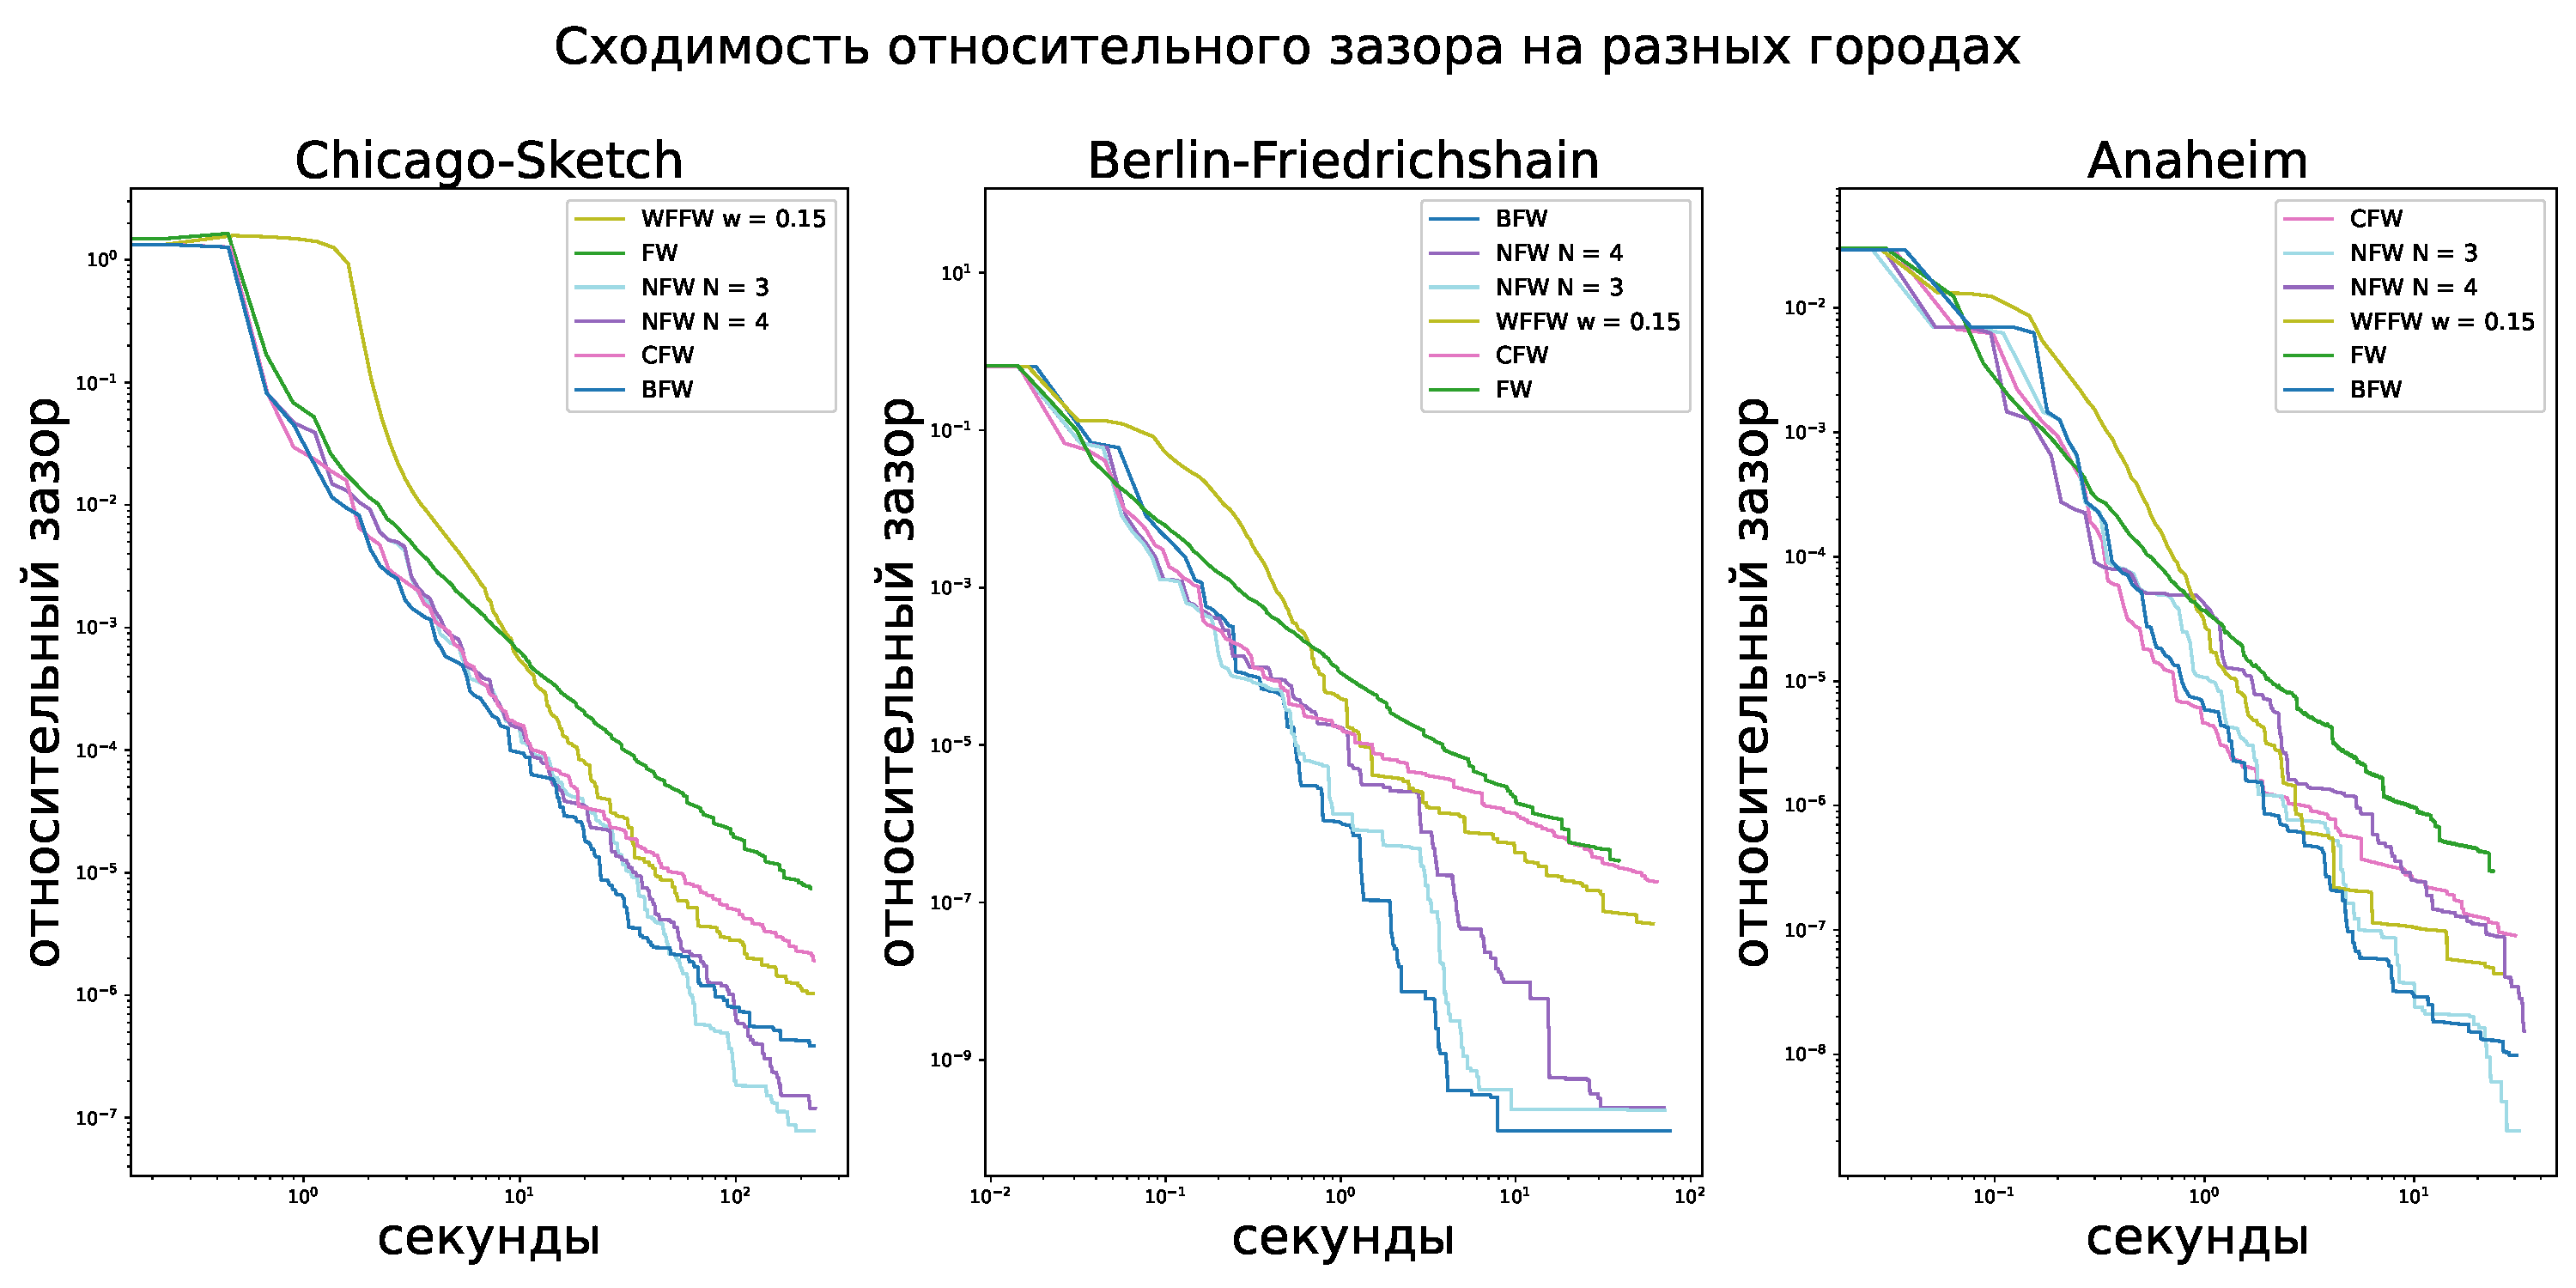
\includegraphics[width=0.98\textwidth]{fw_modifications/0_CFW.pdf}
\caption{Сходимость относительного зазора для NFW, CFW, BFW, WFFW и FW на сетях Chicago-Sketch, Berlin-Friedrichshain и Anaheim.}
\label{fig:fw-mod-cfw-0}
\end{figure}

\begin{figure}[H]
\centering
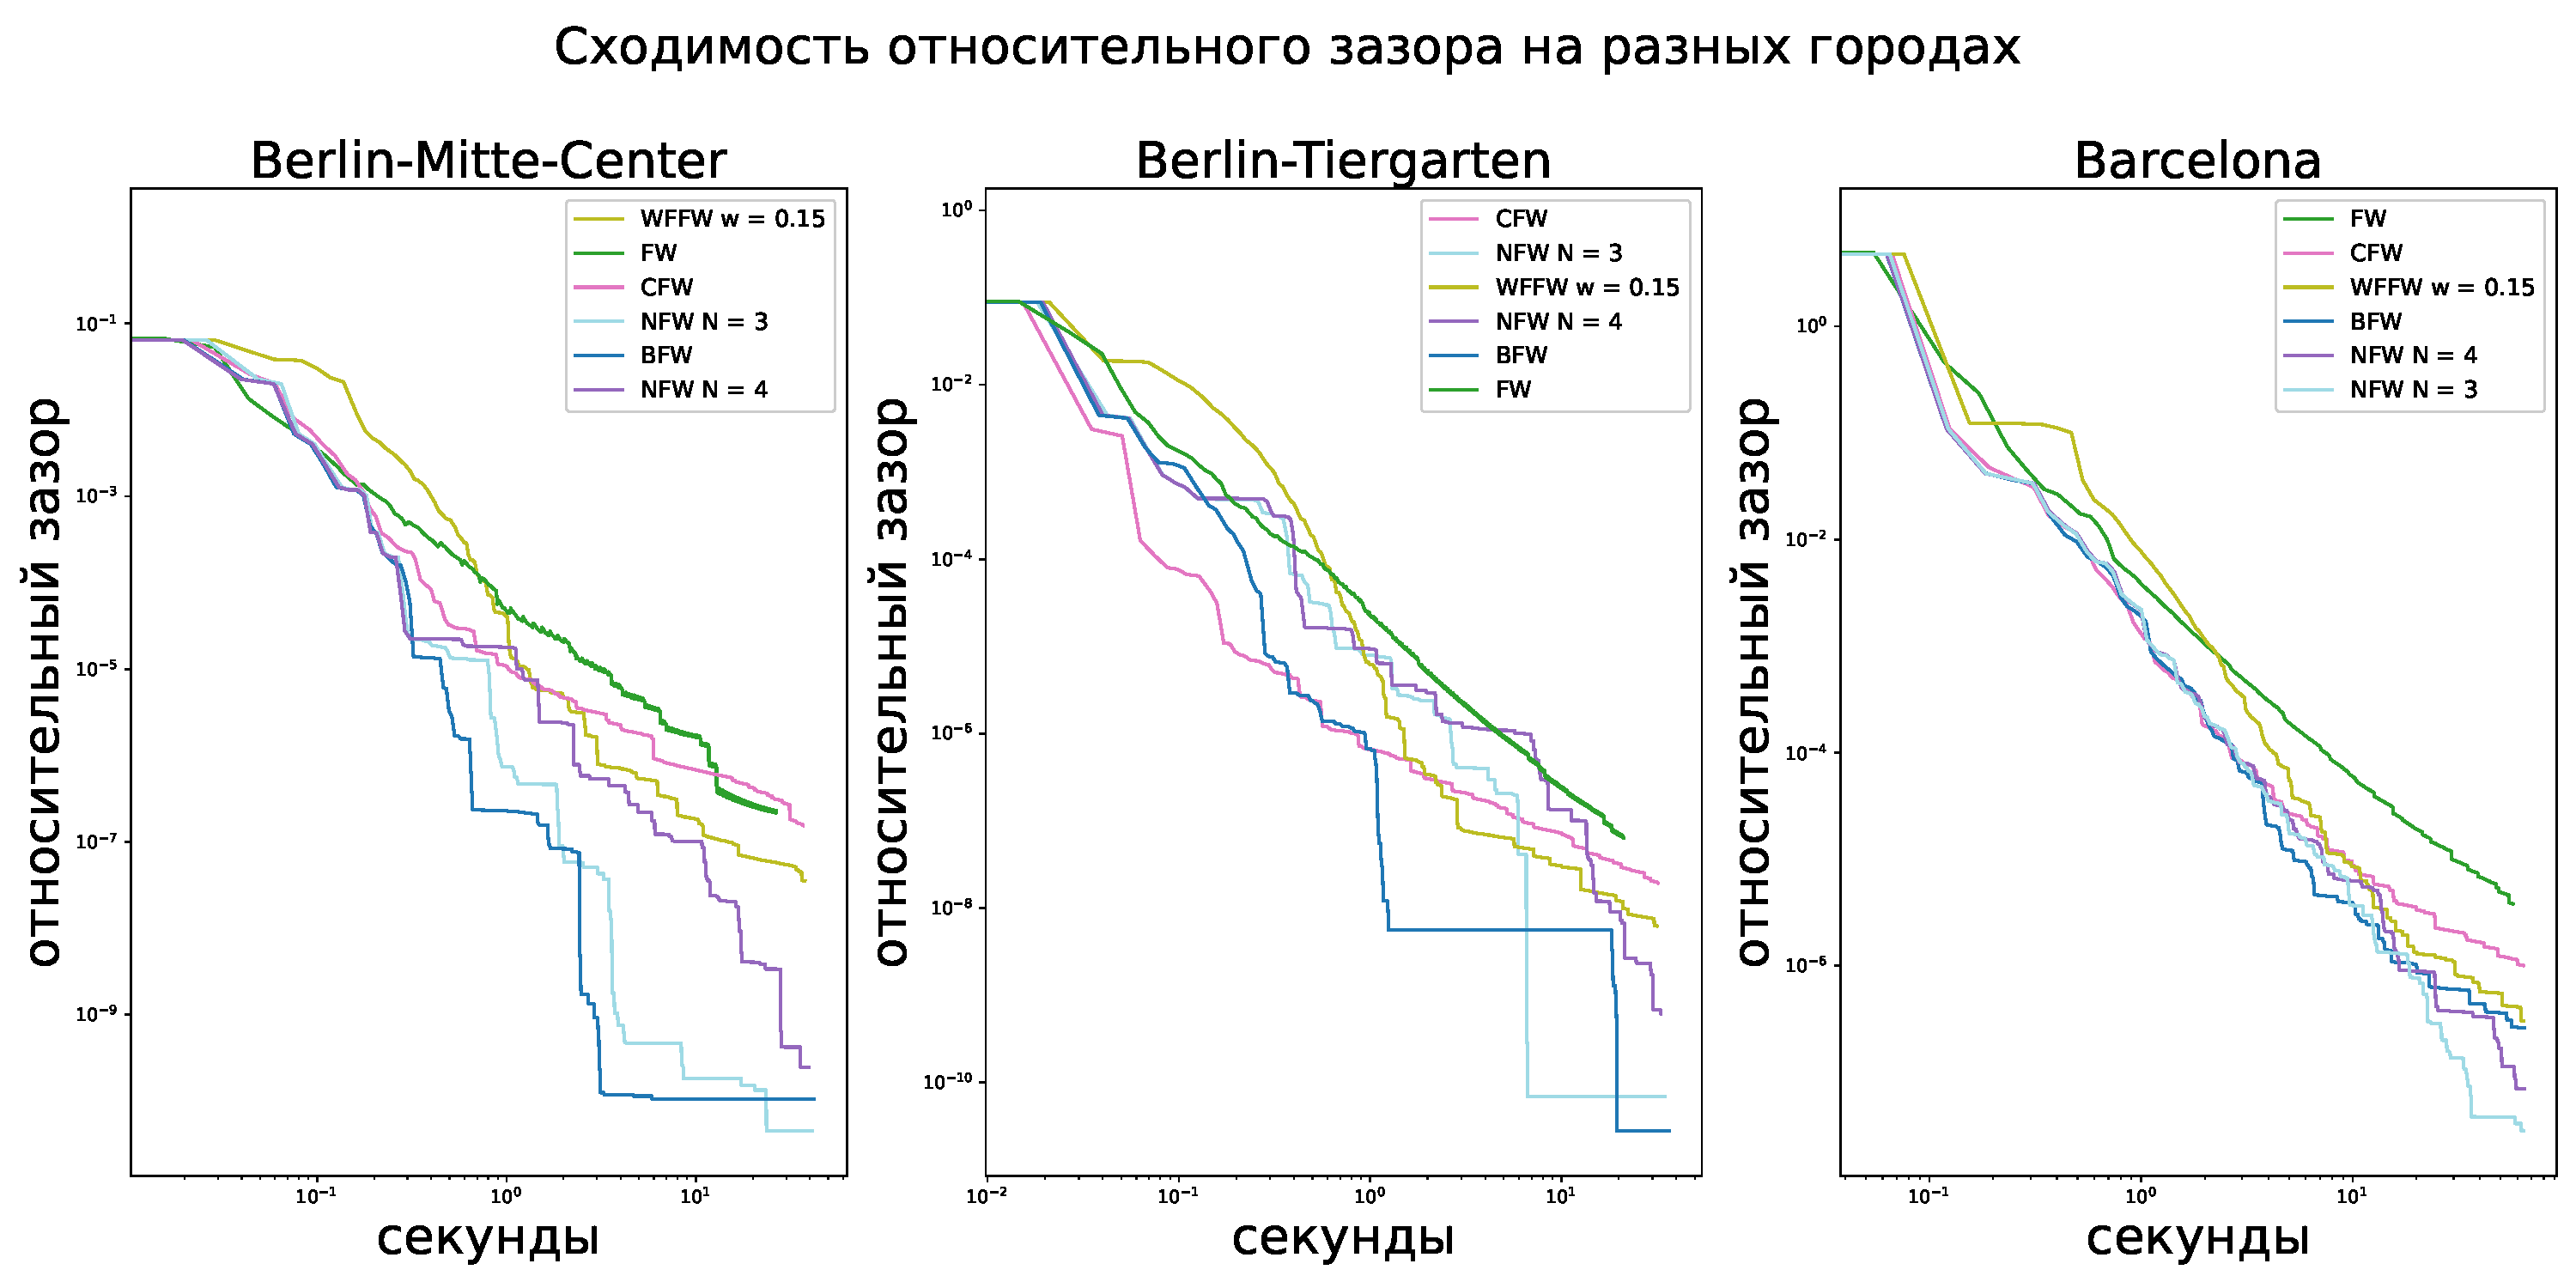
\includegraphics[width=0.98\textwidth]{fw_modifications/3_CFW.pdf}
\caption{Сходимость относительного зазора для NFW, CFW, BFW, WFFW и FW на сетях Berlin-Mitte-Center, Berlin-Tiergarten и Barcelona.}
\label{fig:fw-mod-cfw-3}
\end{figure}

\begin{figure}[H]
\centering
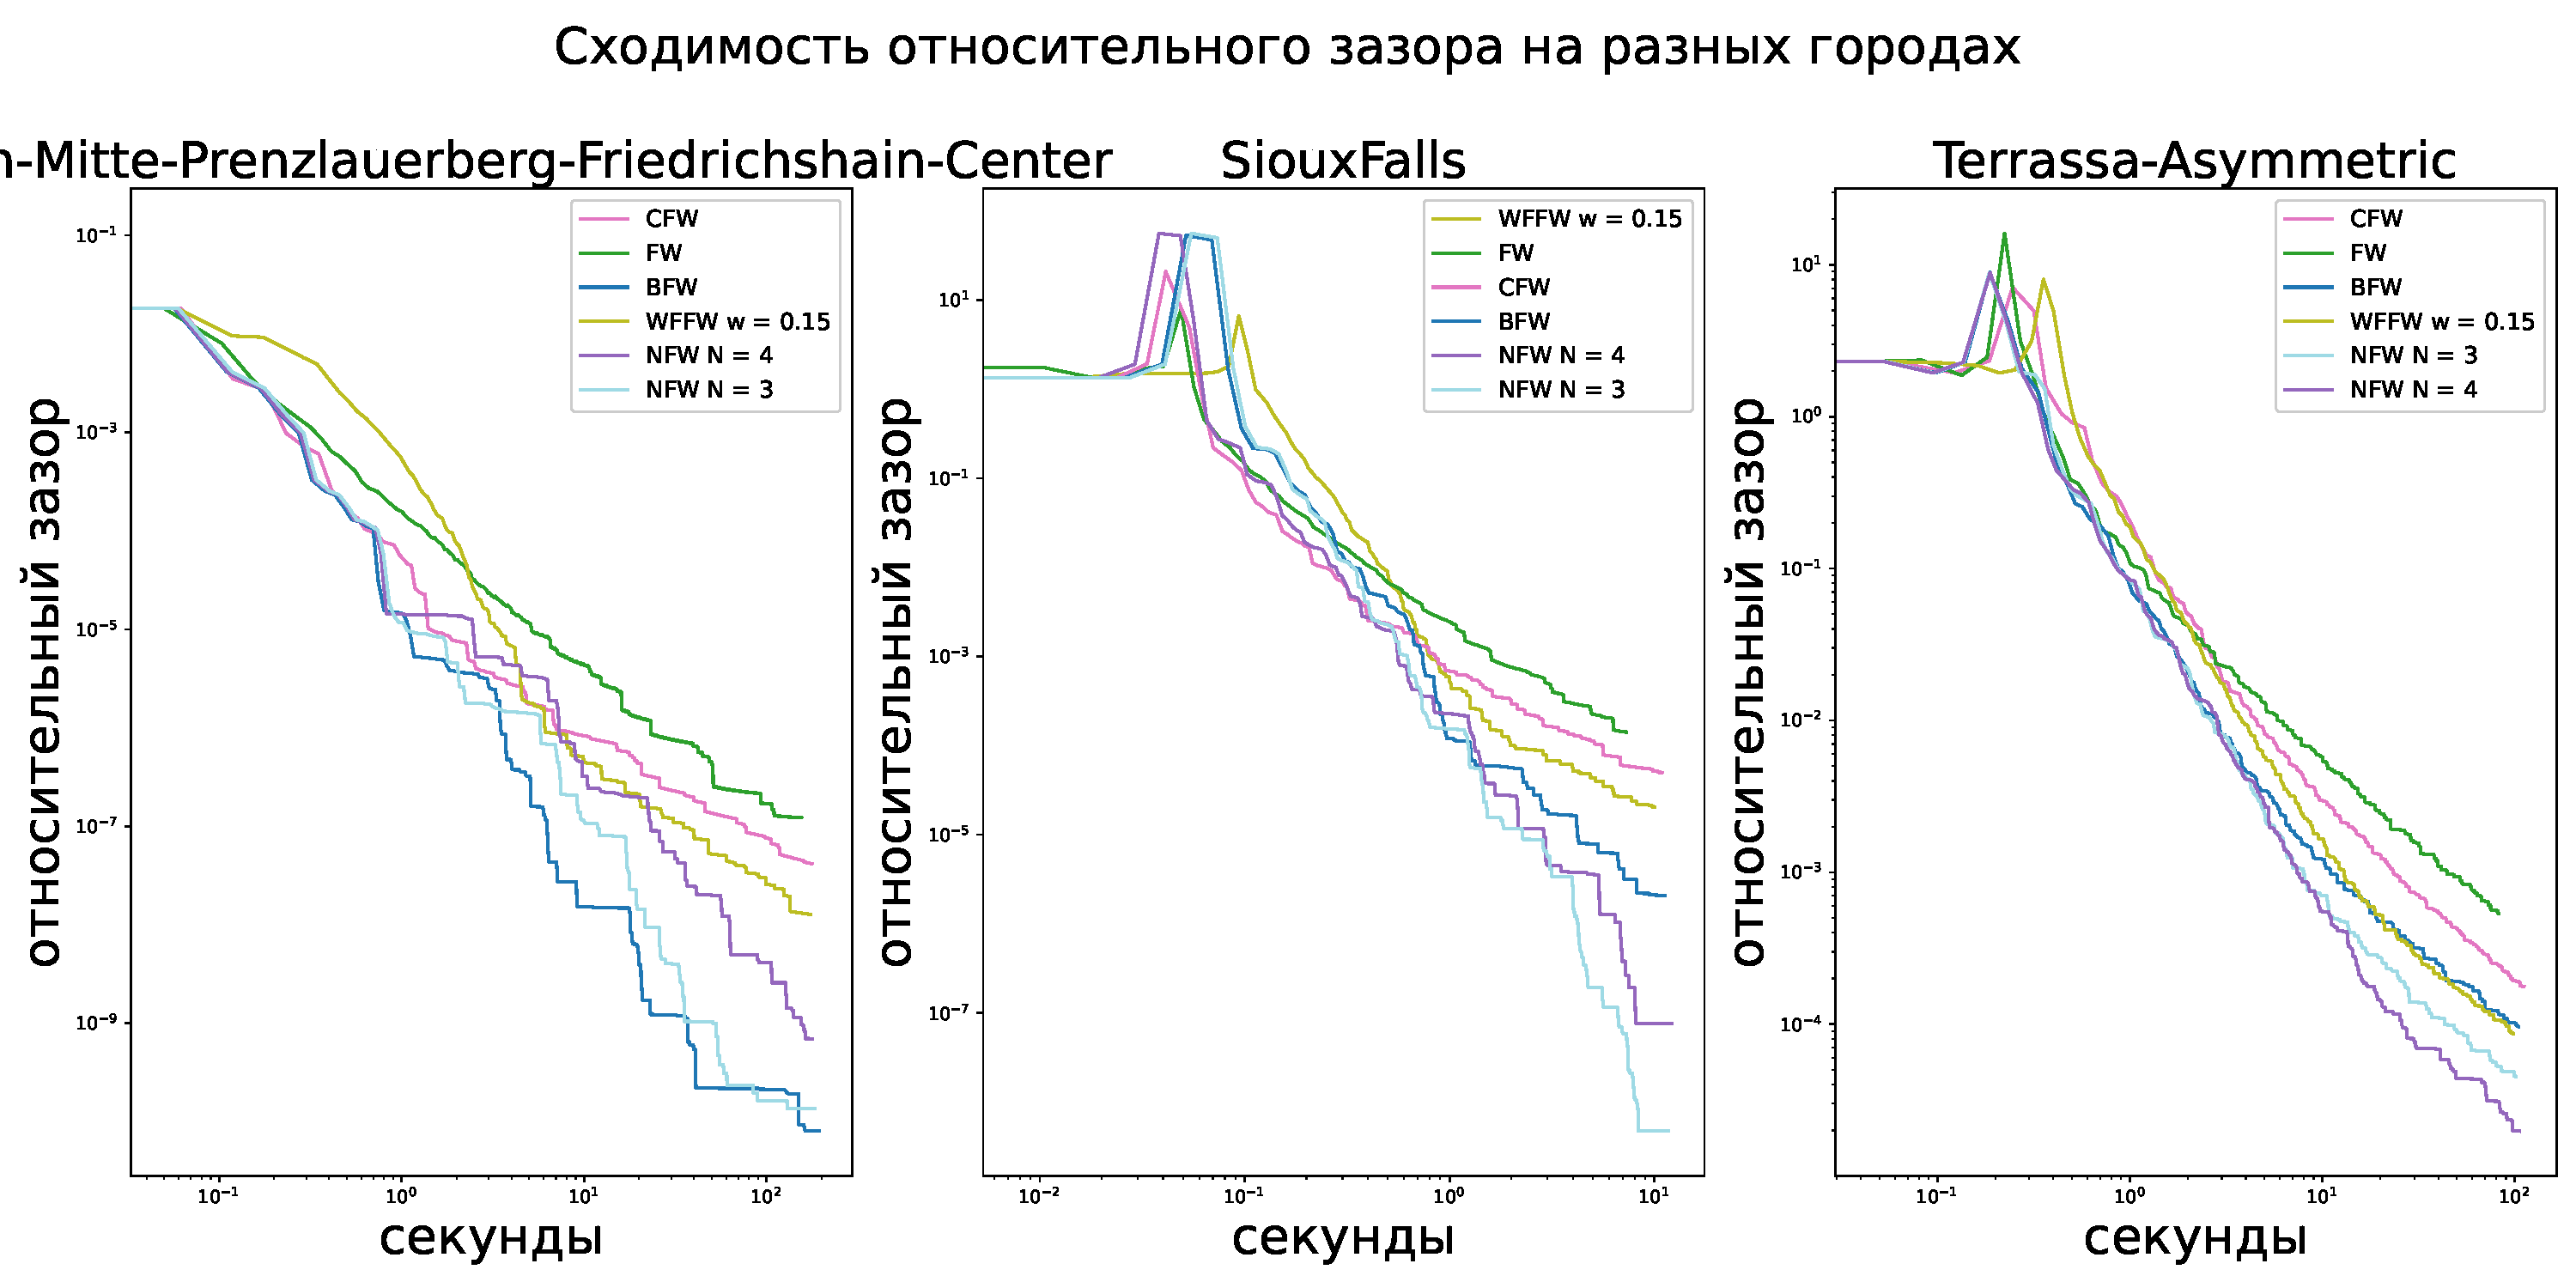
\includegraphics[width=0.98\textwidth]{fw_modifications/8_CFW.pdf}
\caption{Сходимость относительного зазора для NFW, CFW, BFW, WFFW и FW на сетях Berlin-Mitte-Prenzlauerberg-Friedrichshain-Center, SiouxFalls и Terrassa-Asymmetric.}
\label{fig:fw-mod-cfw-8}
\end{figure}

Вторая серия посвящена сравнению Fukushima Frank--Wolfe и Weighted Fukushima Frank--Wolfe.
Здесь проверяется, насколько простое сглаживание направлений может конкурировать с
сопряженными методами.
Равномерное усреднение FFW стабилизирует траекторию, но может запаздывать, поскольку старые
направления удерживают алгоритм в области, которая уже не соответствует текущим кратчайшим
путям.
WFFW исправляет эту особенность с помощью геометрического забывания.
Результаты приведены на рис.~\ref{fig:fw-mod-wffw-0}--\ref{fig:fw-mod-wffw-2}.

\begin{figure}[H]
\centering
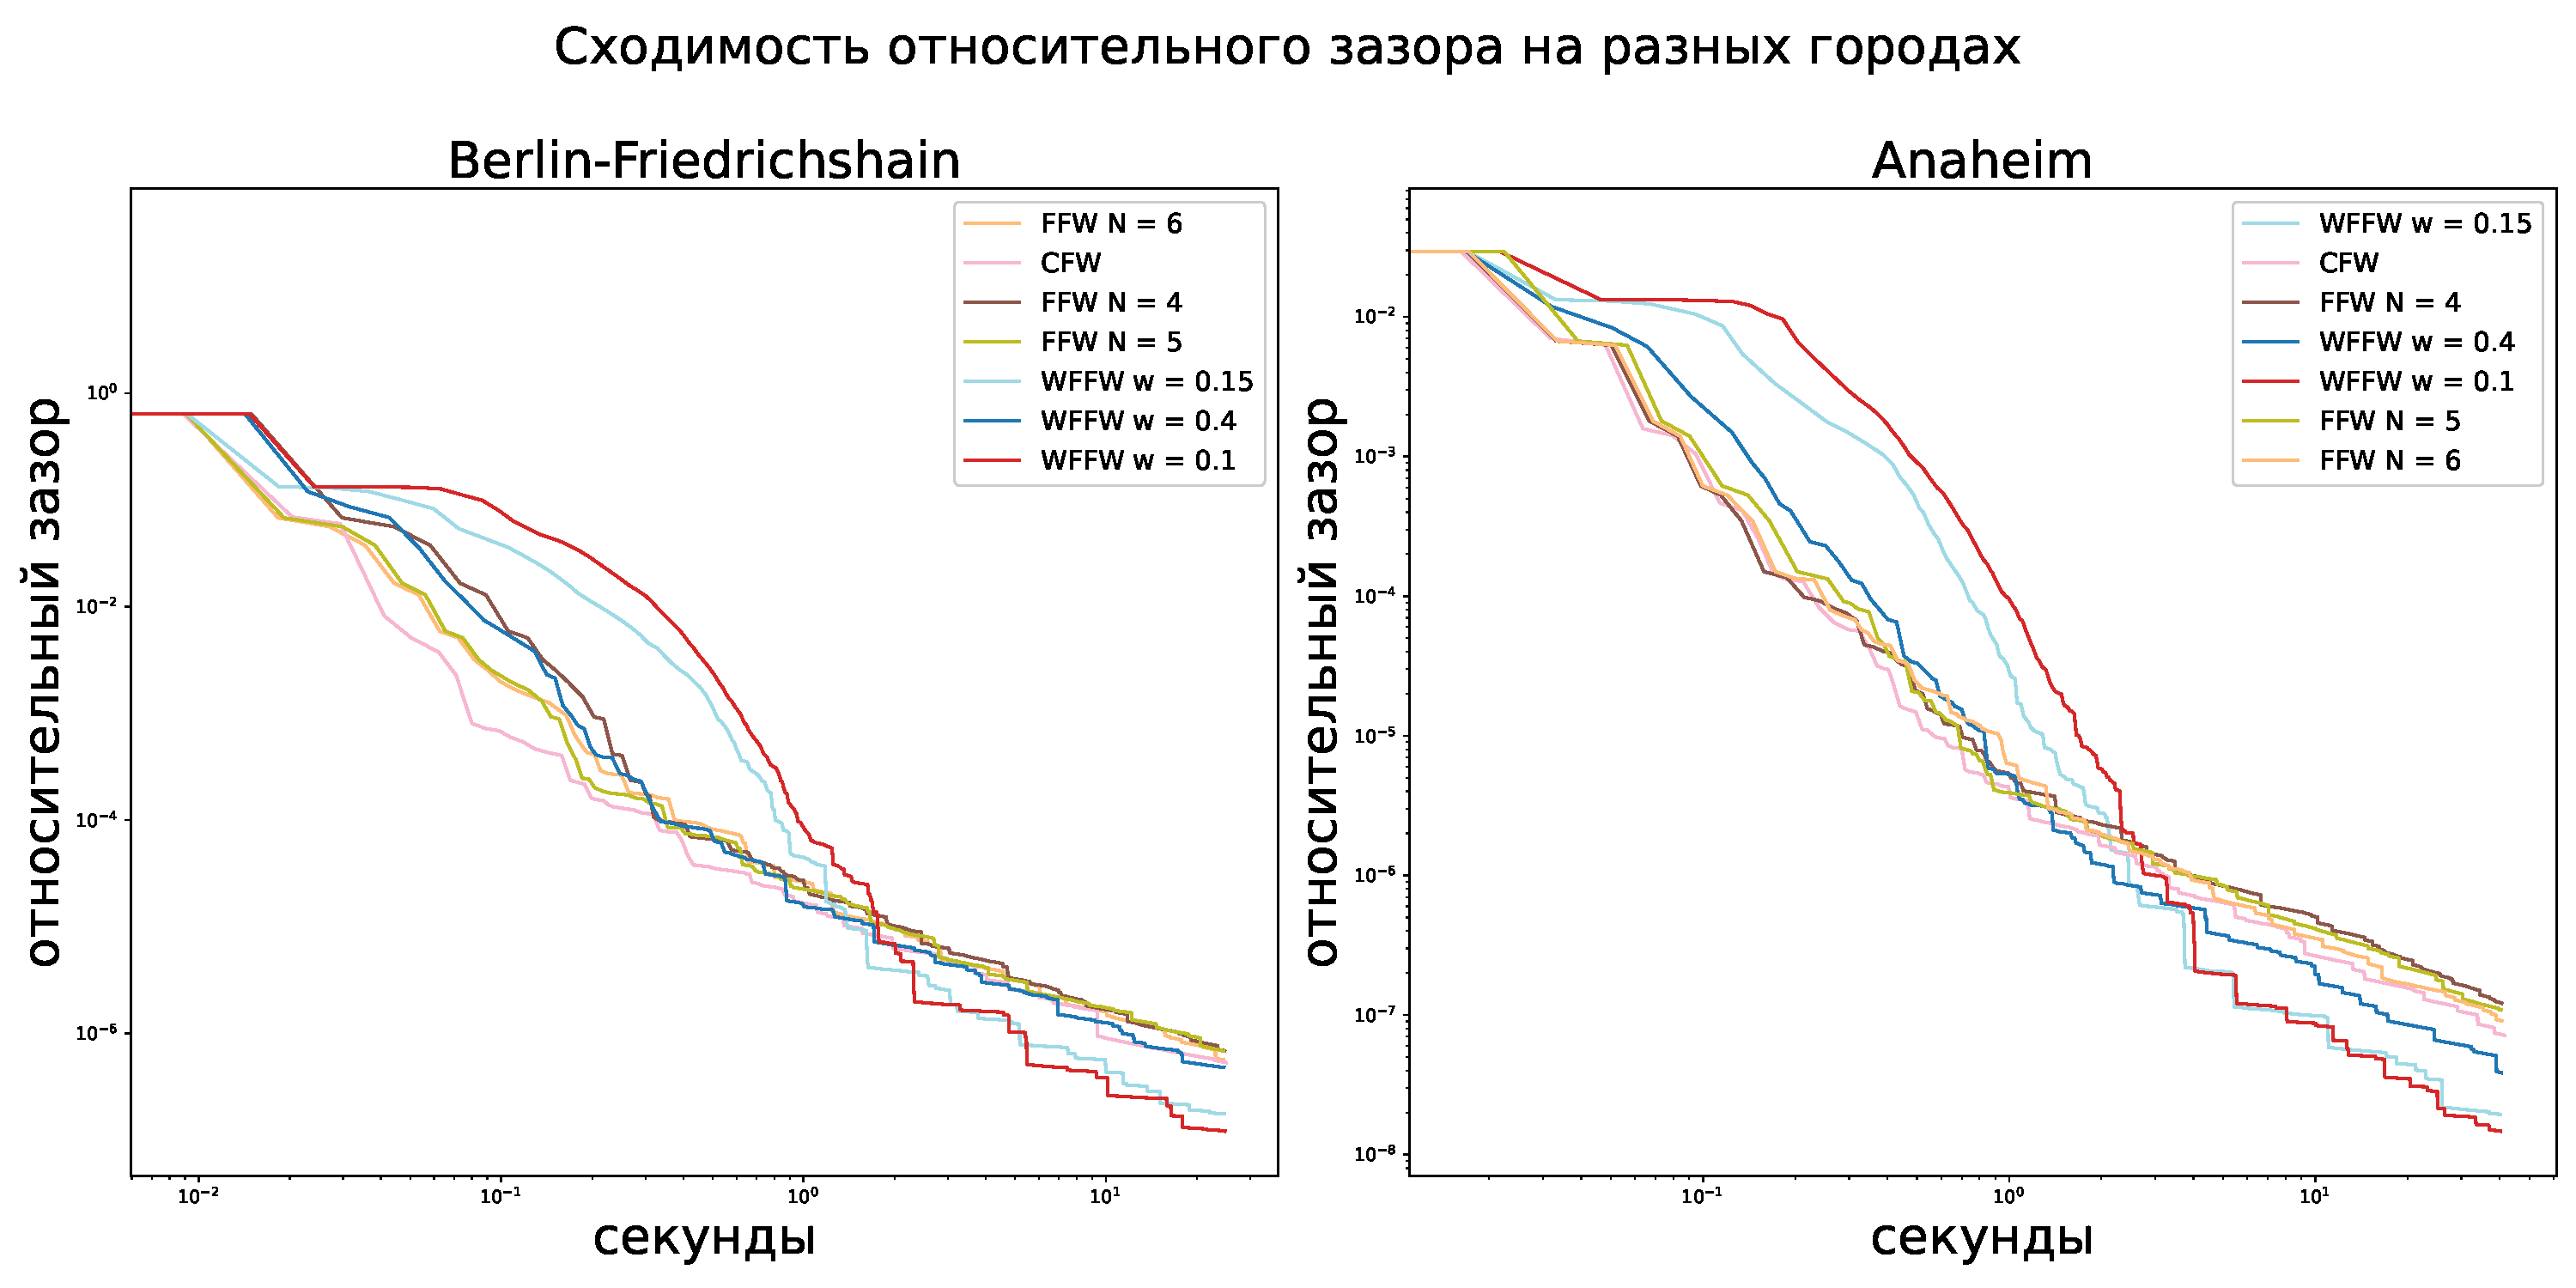
\includegraphics[width=0.98\textwidth]{fw_modifications/0_WFW_weighted.pdf}
\caption{Сравнение FFW, WFFW и CFW по относительному зазору на сетях Anaheim и Berlin-Friedrichshain.}
\label{fig:fw-mod-wffw-0}
\end{figure}

\begin{figure}[H]
\centering
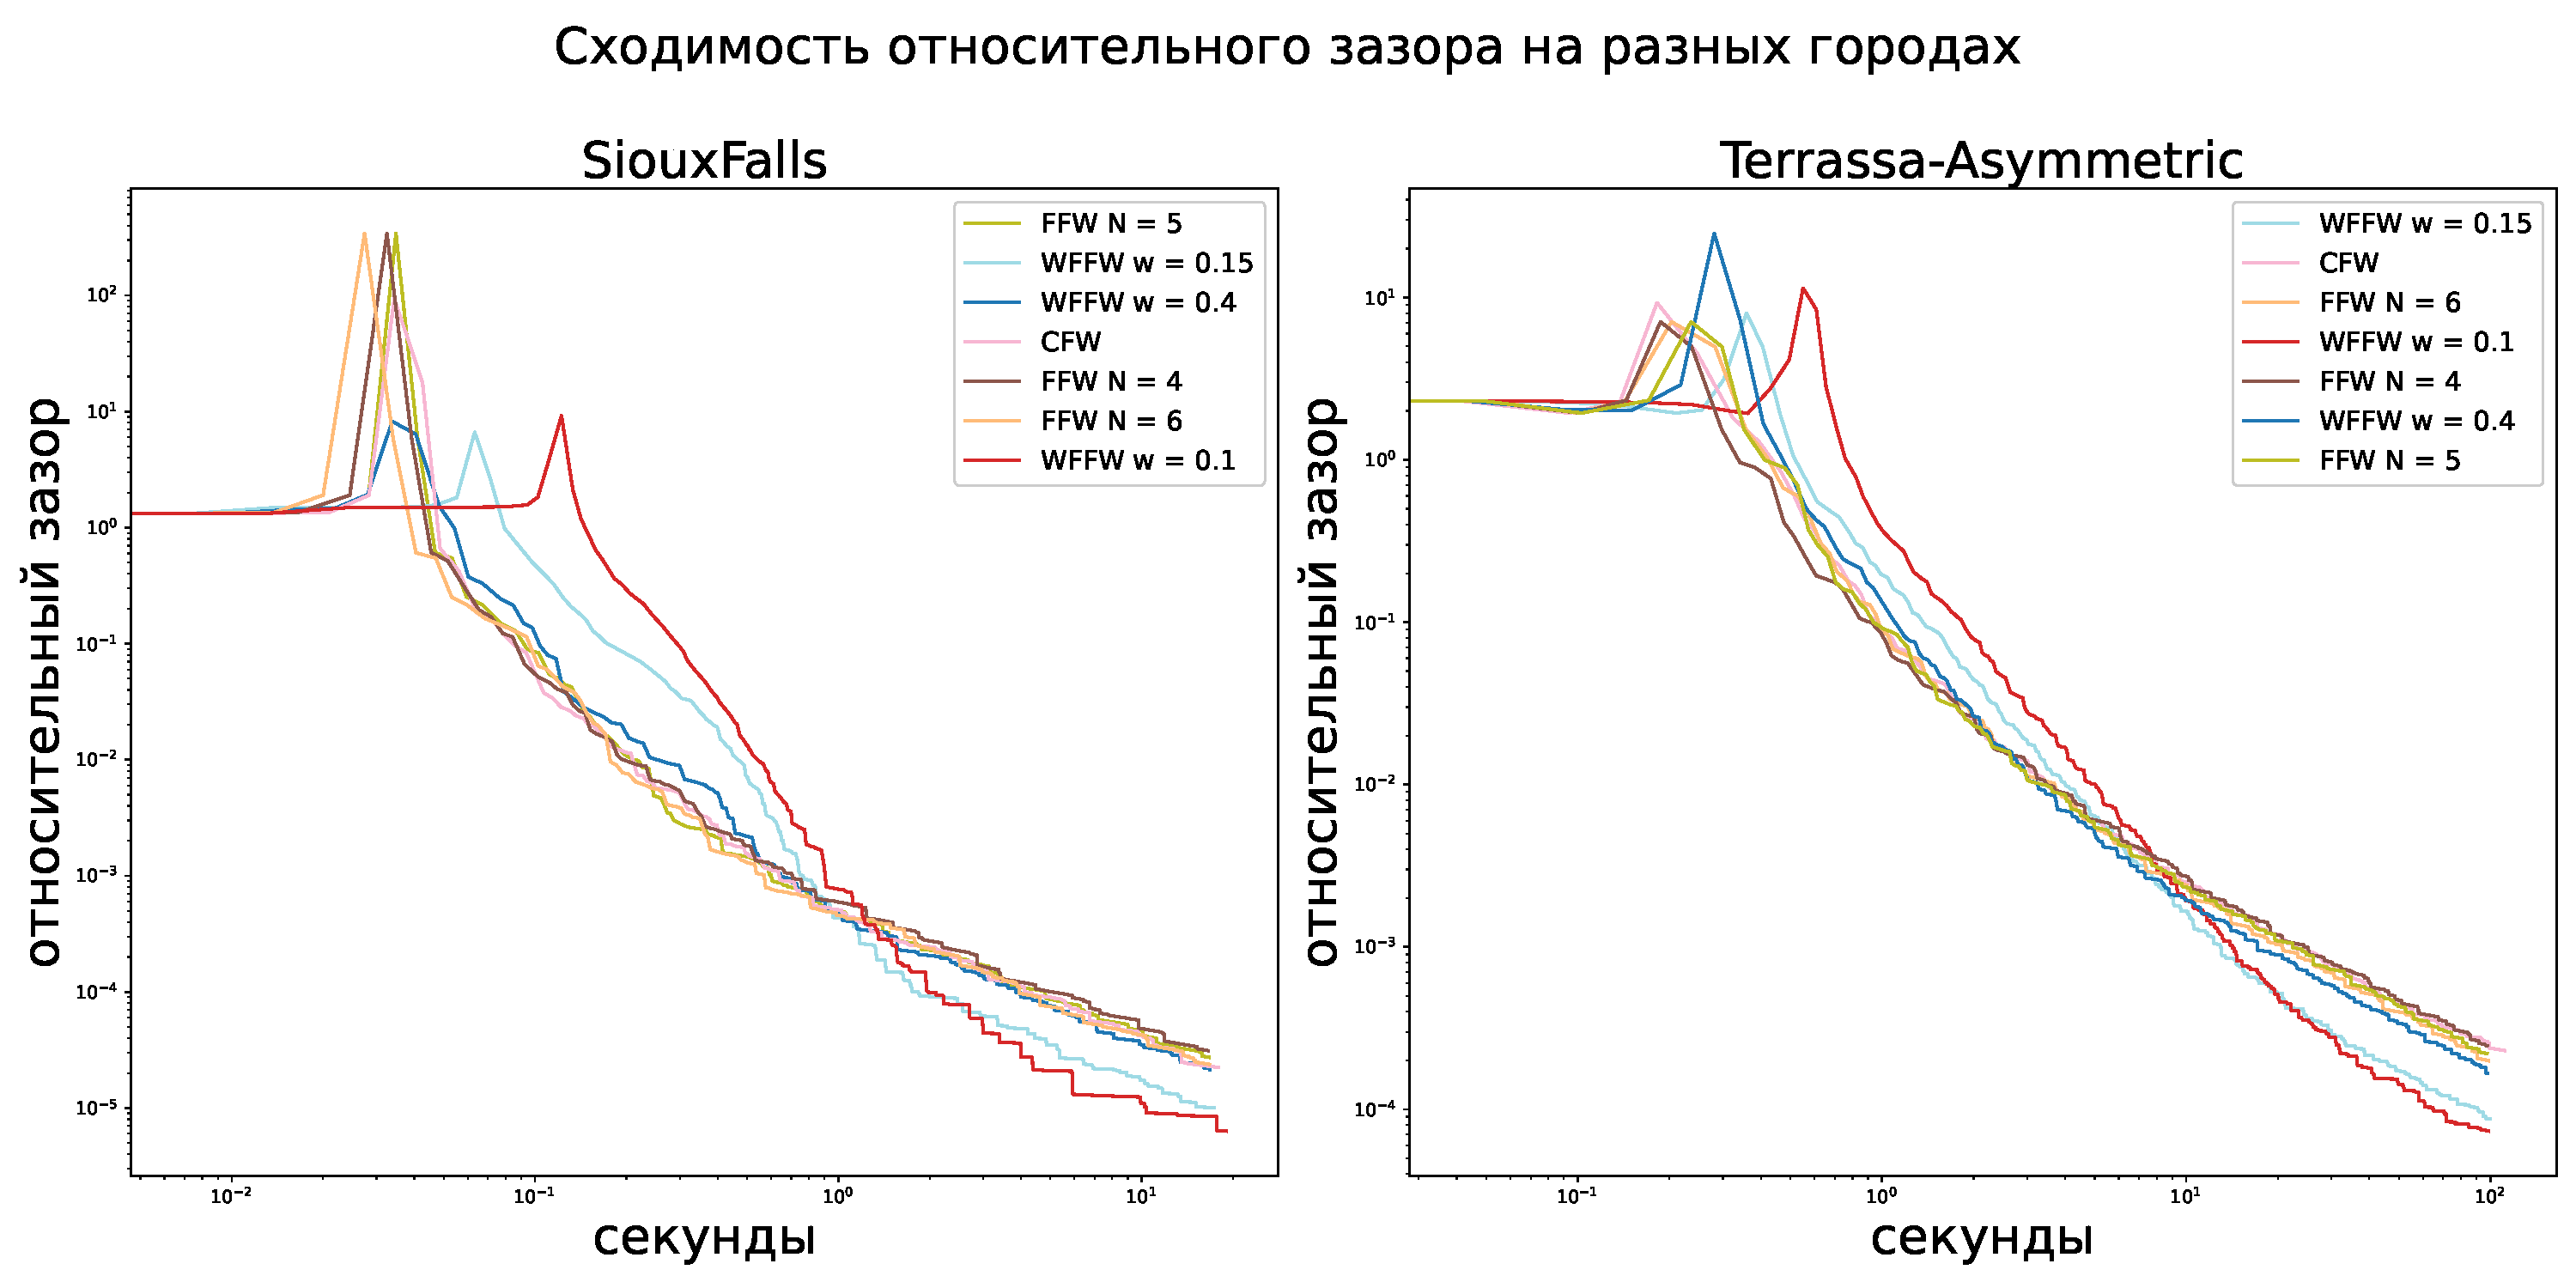
\includegraphics[width=0.98\textwidth]{fw_modifications/2_WFW_weighted.pdf}
\caption{Сравнение FFW, WFFW и CFW по относительному зазору на сетях SiouxFalls и Terrassa-Asymmetric.}
\label{fig:fw-mod-wffw-2}
\end{figure}

Третья серия меняет глубину памяти NFW.
Сравниваются варианты с разным числом предыдущих направлений.
При $N=2$ метод совпадает по смыслу с BFW, а при больших $N$ начинает использовать более
длинную историю направлений.
На рис.~\ref{fig:fw-mod-nfw-0}--\ref{fig:fw-mod-nfw-2} видно, что увеличение глубины памяти
может давать дополнительное ускорение, но эффект зависит от сети: слишком старые направления
иногда описывают уже неактуальную локальную геометрию задачи.

\begin{figure}[H]
\centering
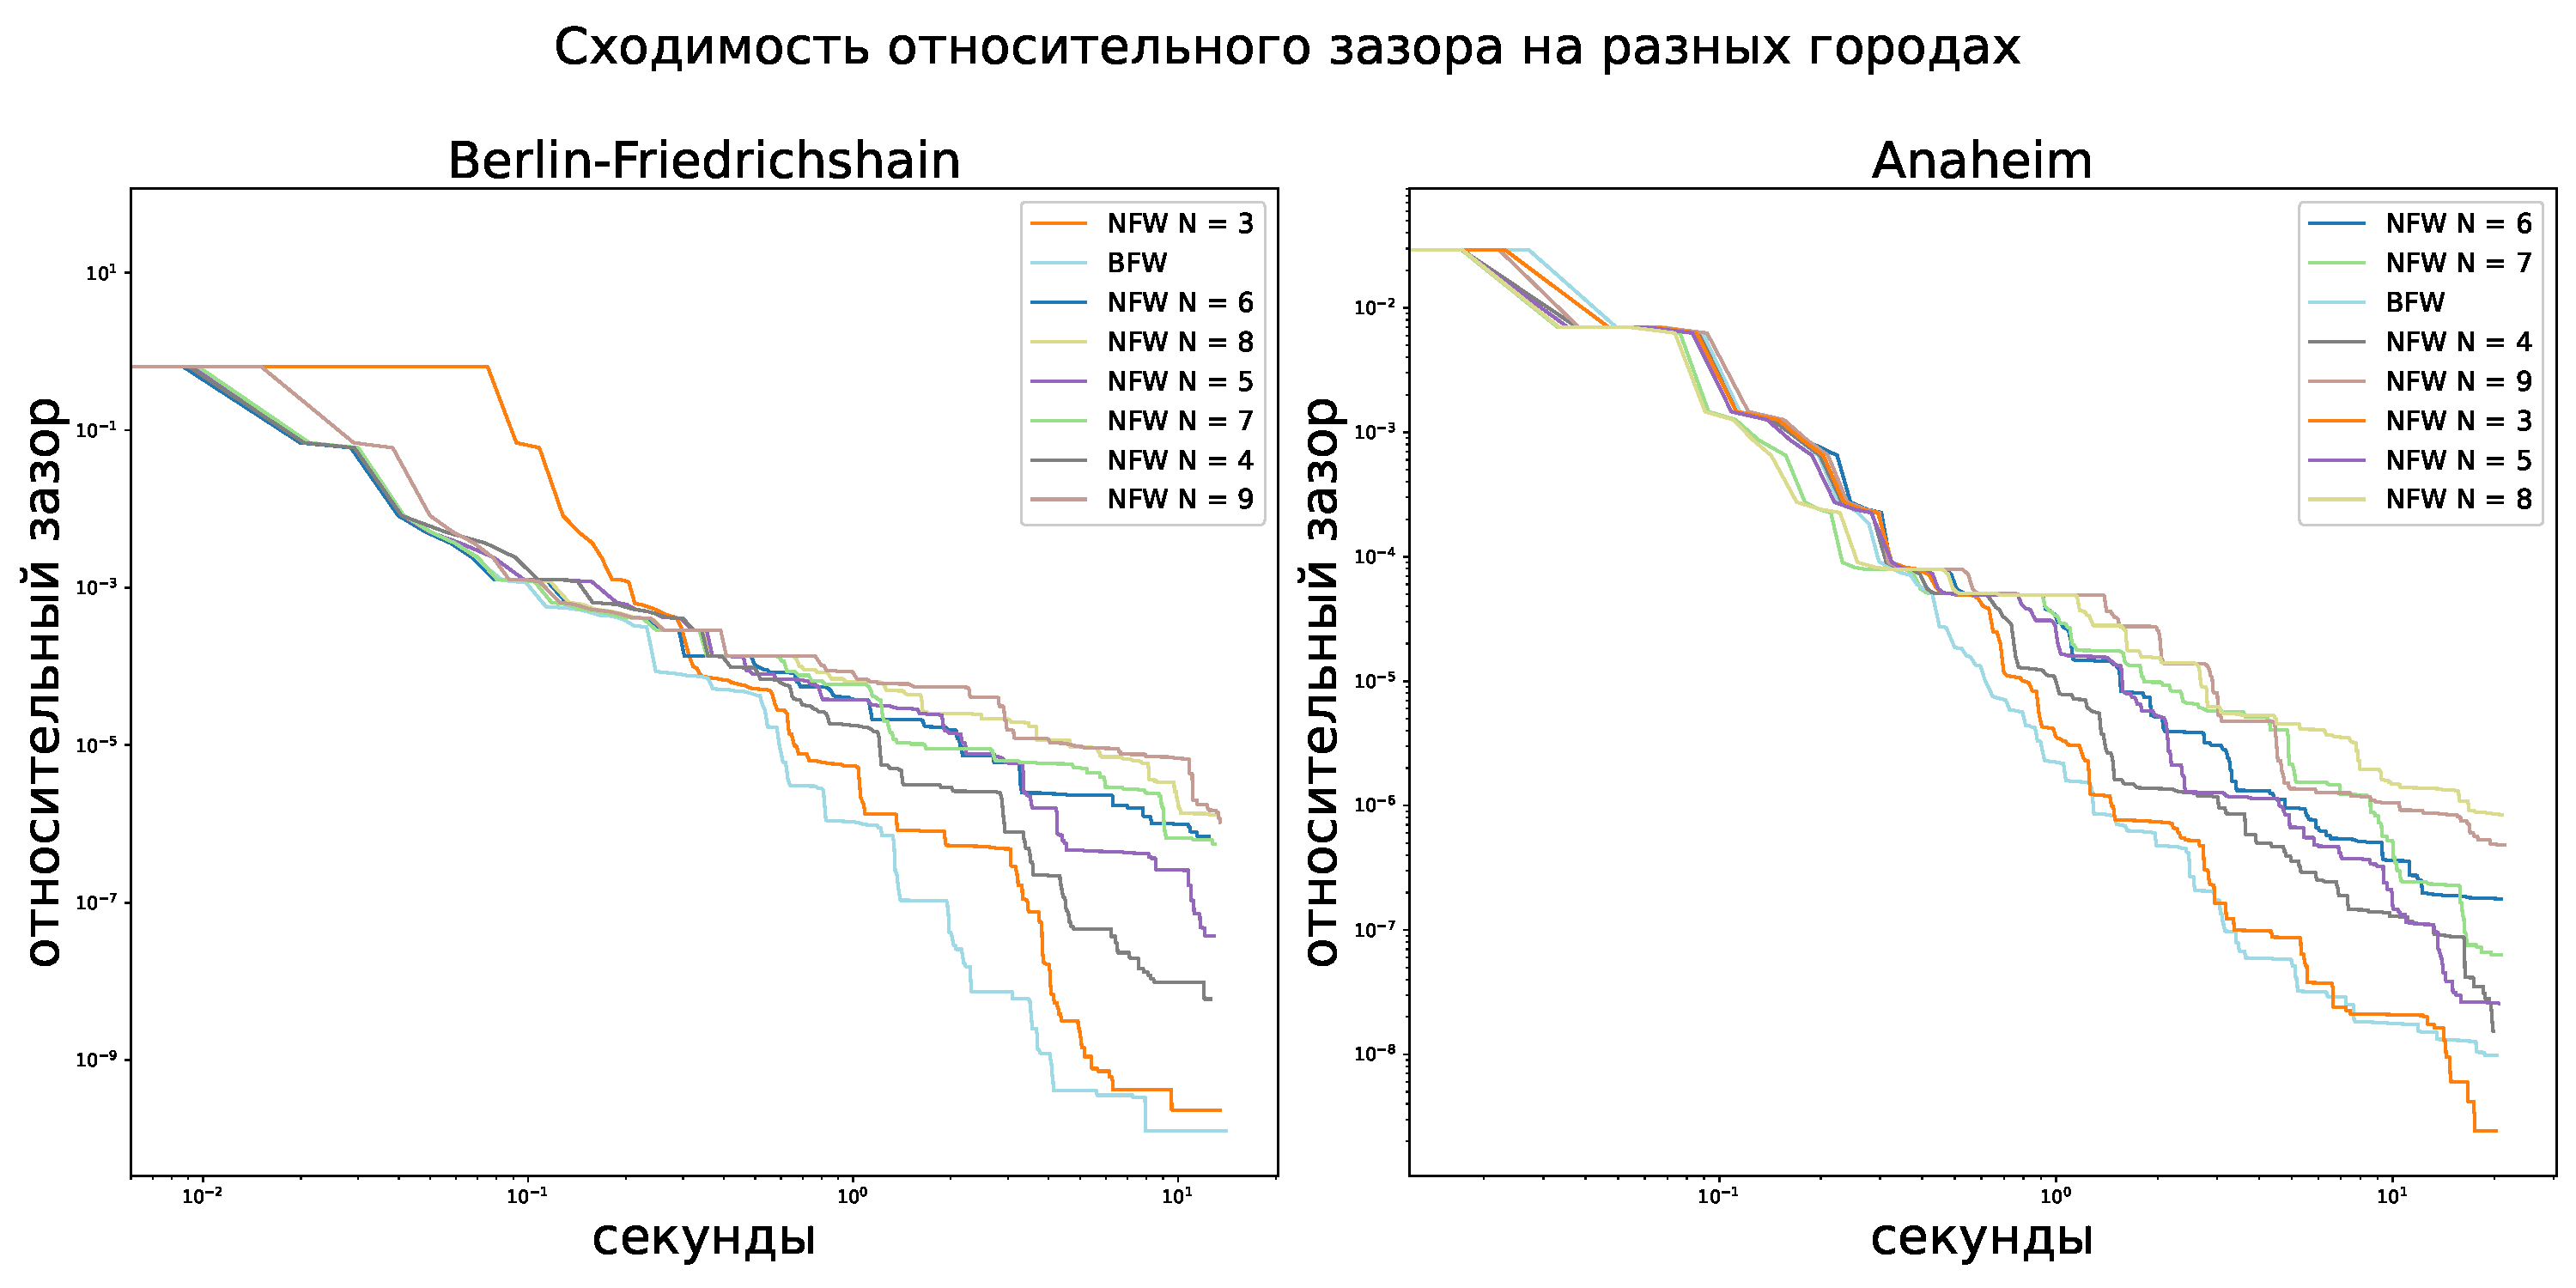
\includegraphics[width=0.98\textwidth]{fw_modifications/0_NFW.pdf}
\caption{Сравнение NFW с разной глубиной памяти и BFW на сетях Anaheim и Berlin-Friedrichshain.}
\label{fig:fw-mod-nfw-0}
\end{figure}

\begin{figure}[H]
\centering
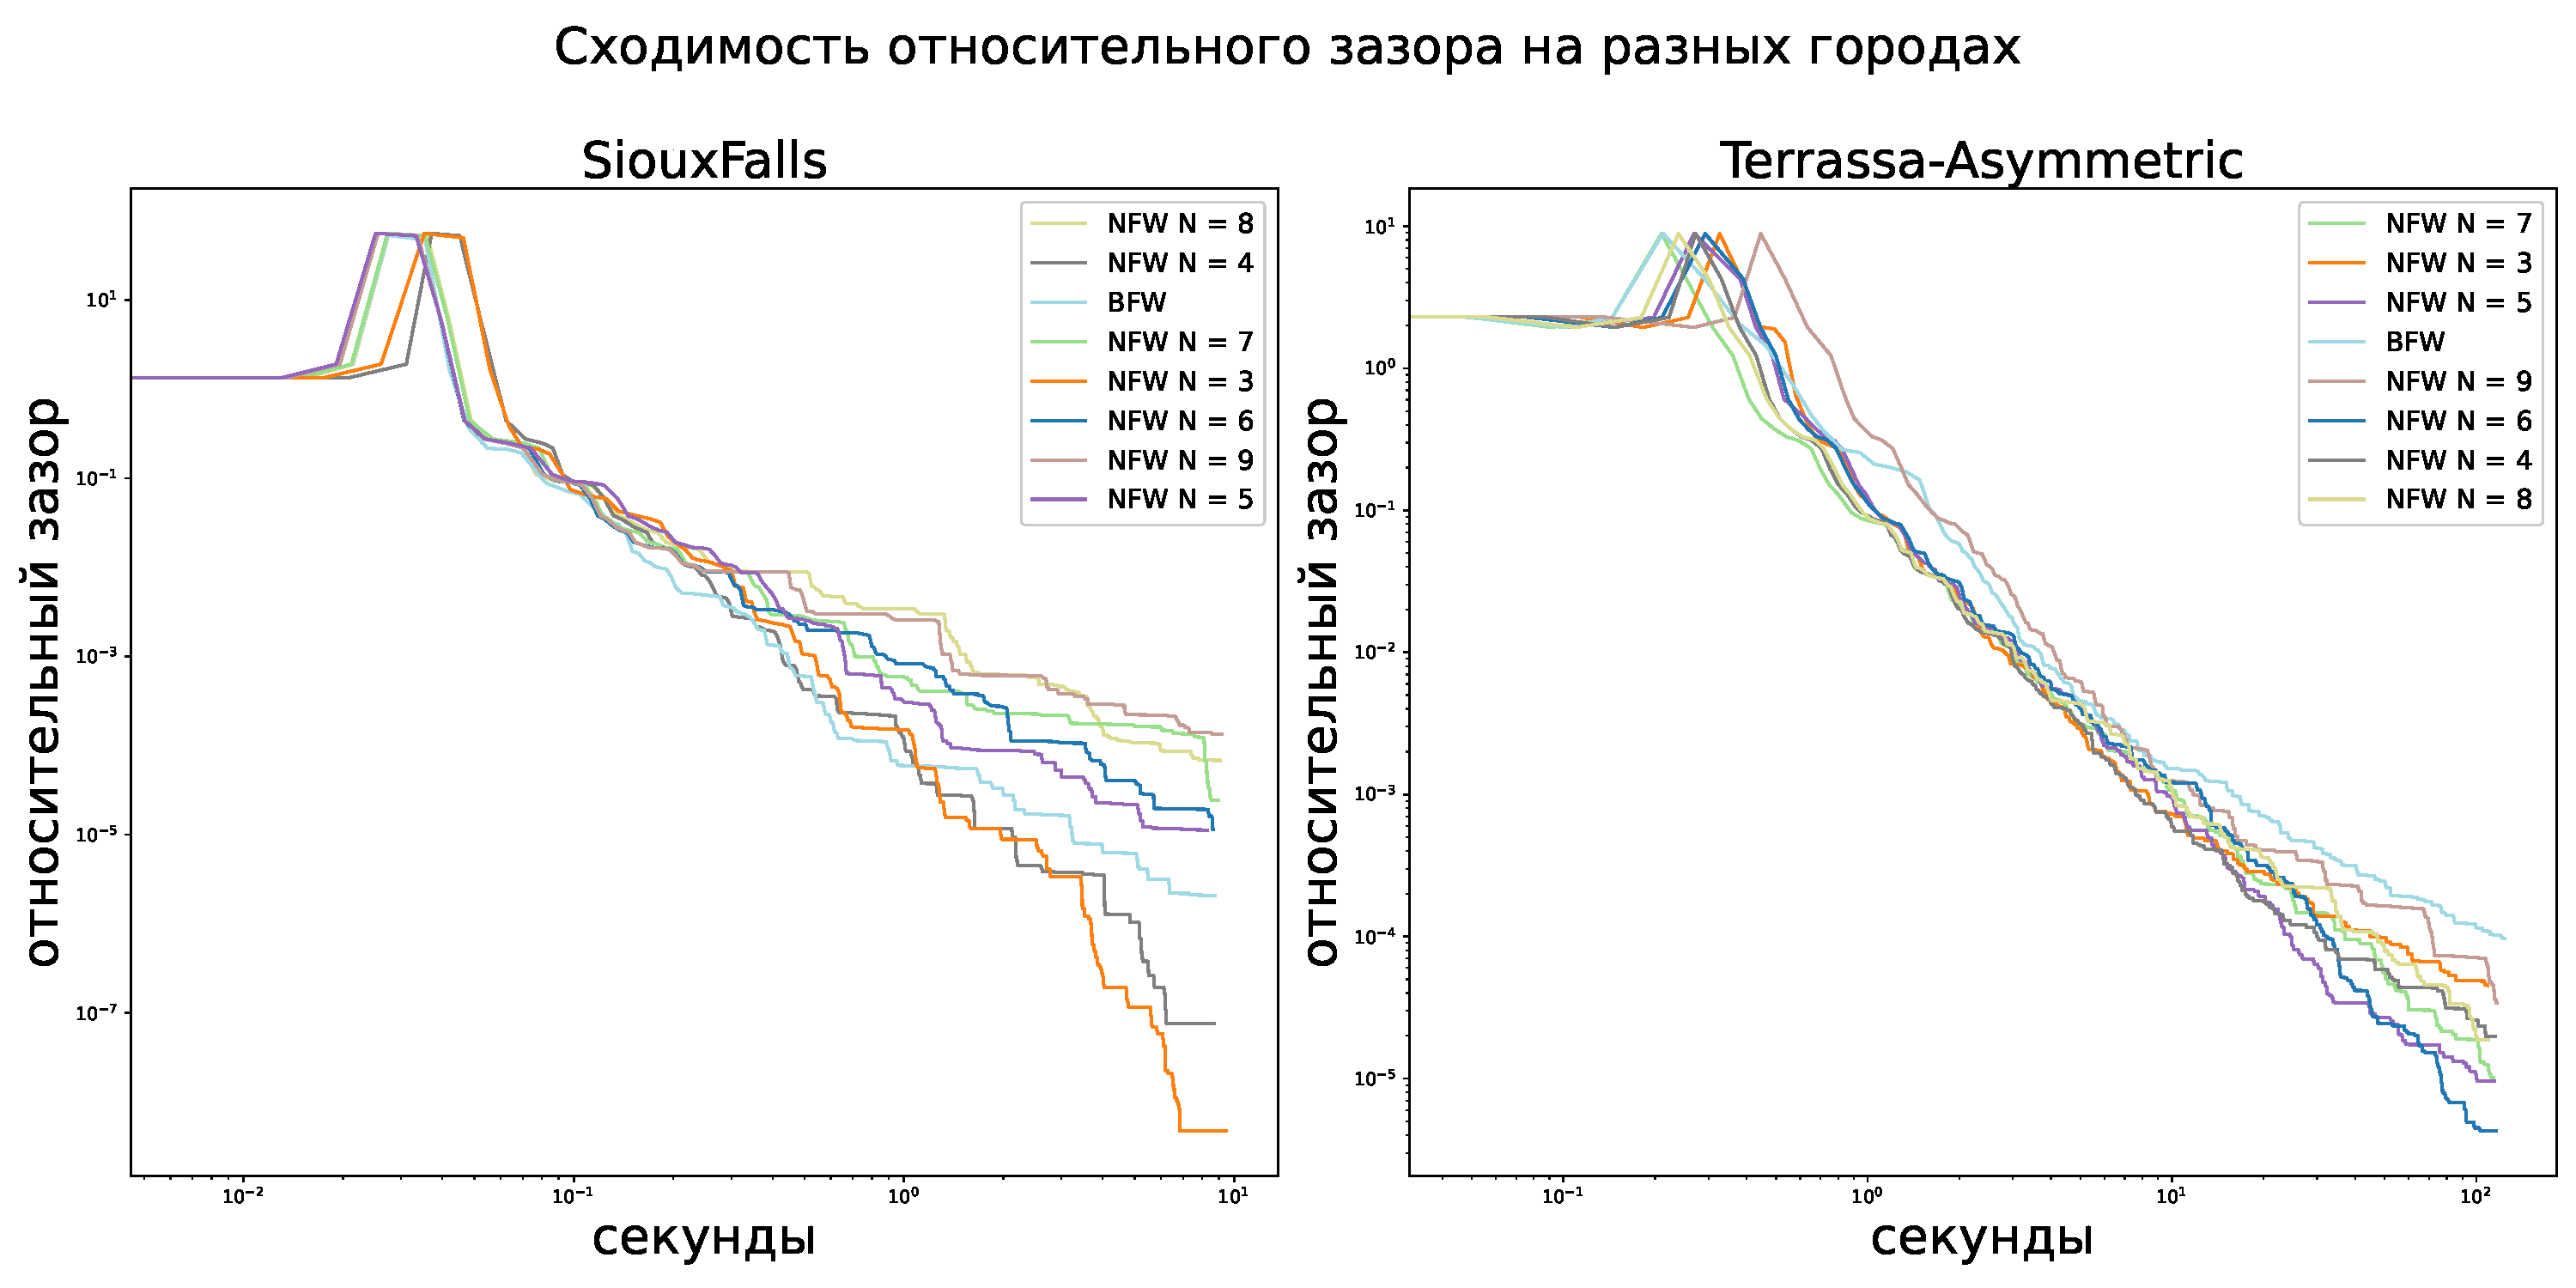
\includegraphics[width=0.98\textwidth]{fw_modifications/2_NFW.pdf}
\caption{Сравнение NFW с разной глубиной памяти и BFW на сетях SiouxFalls и Terrassa-Asymmetric.}
\label{fig:fw-mod-nfw-2}
\end{figure}

Четвертая серия проверяет параметры WFFW.
Если вес текущего FW-направления слишком мал, метод двигается инерционно и может медленно
реагировать на изменение кратчайших путей.
Если этот вес слишком велик, метод почти совпадает с FW и теряет смысл сглаживания.
На рис.~\ref{fig:fw-mod-wffw-params} показано, что нужен баланс между новым FW-направлением
и памятью о прошлых направлениях.

\begin{figure}[H]
\centering
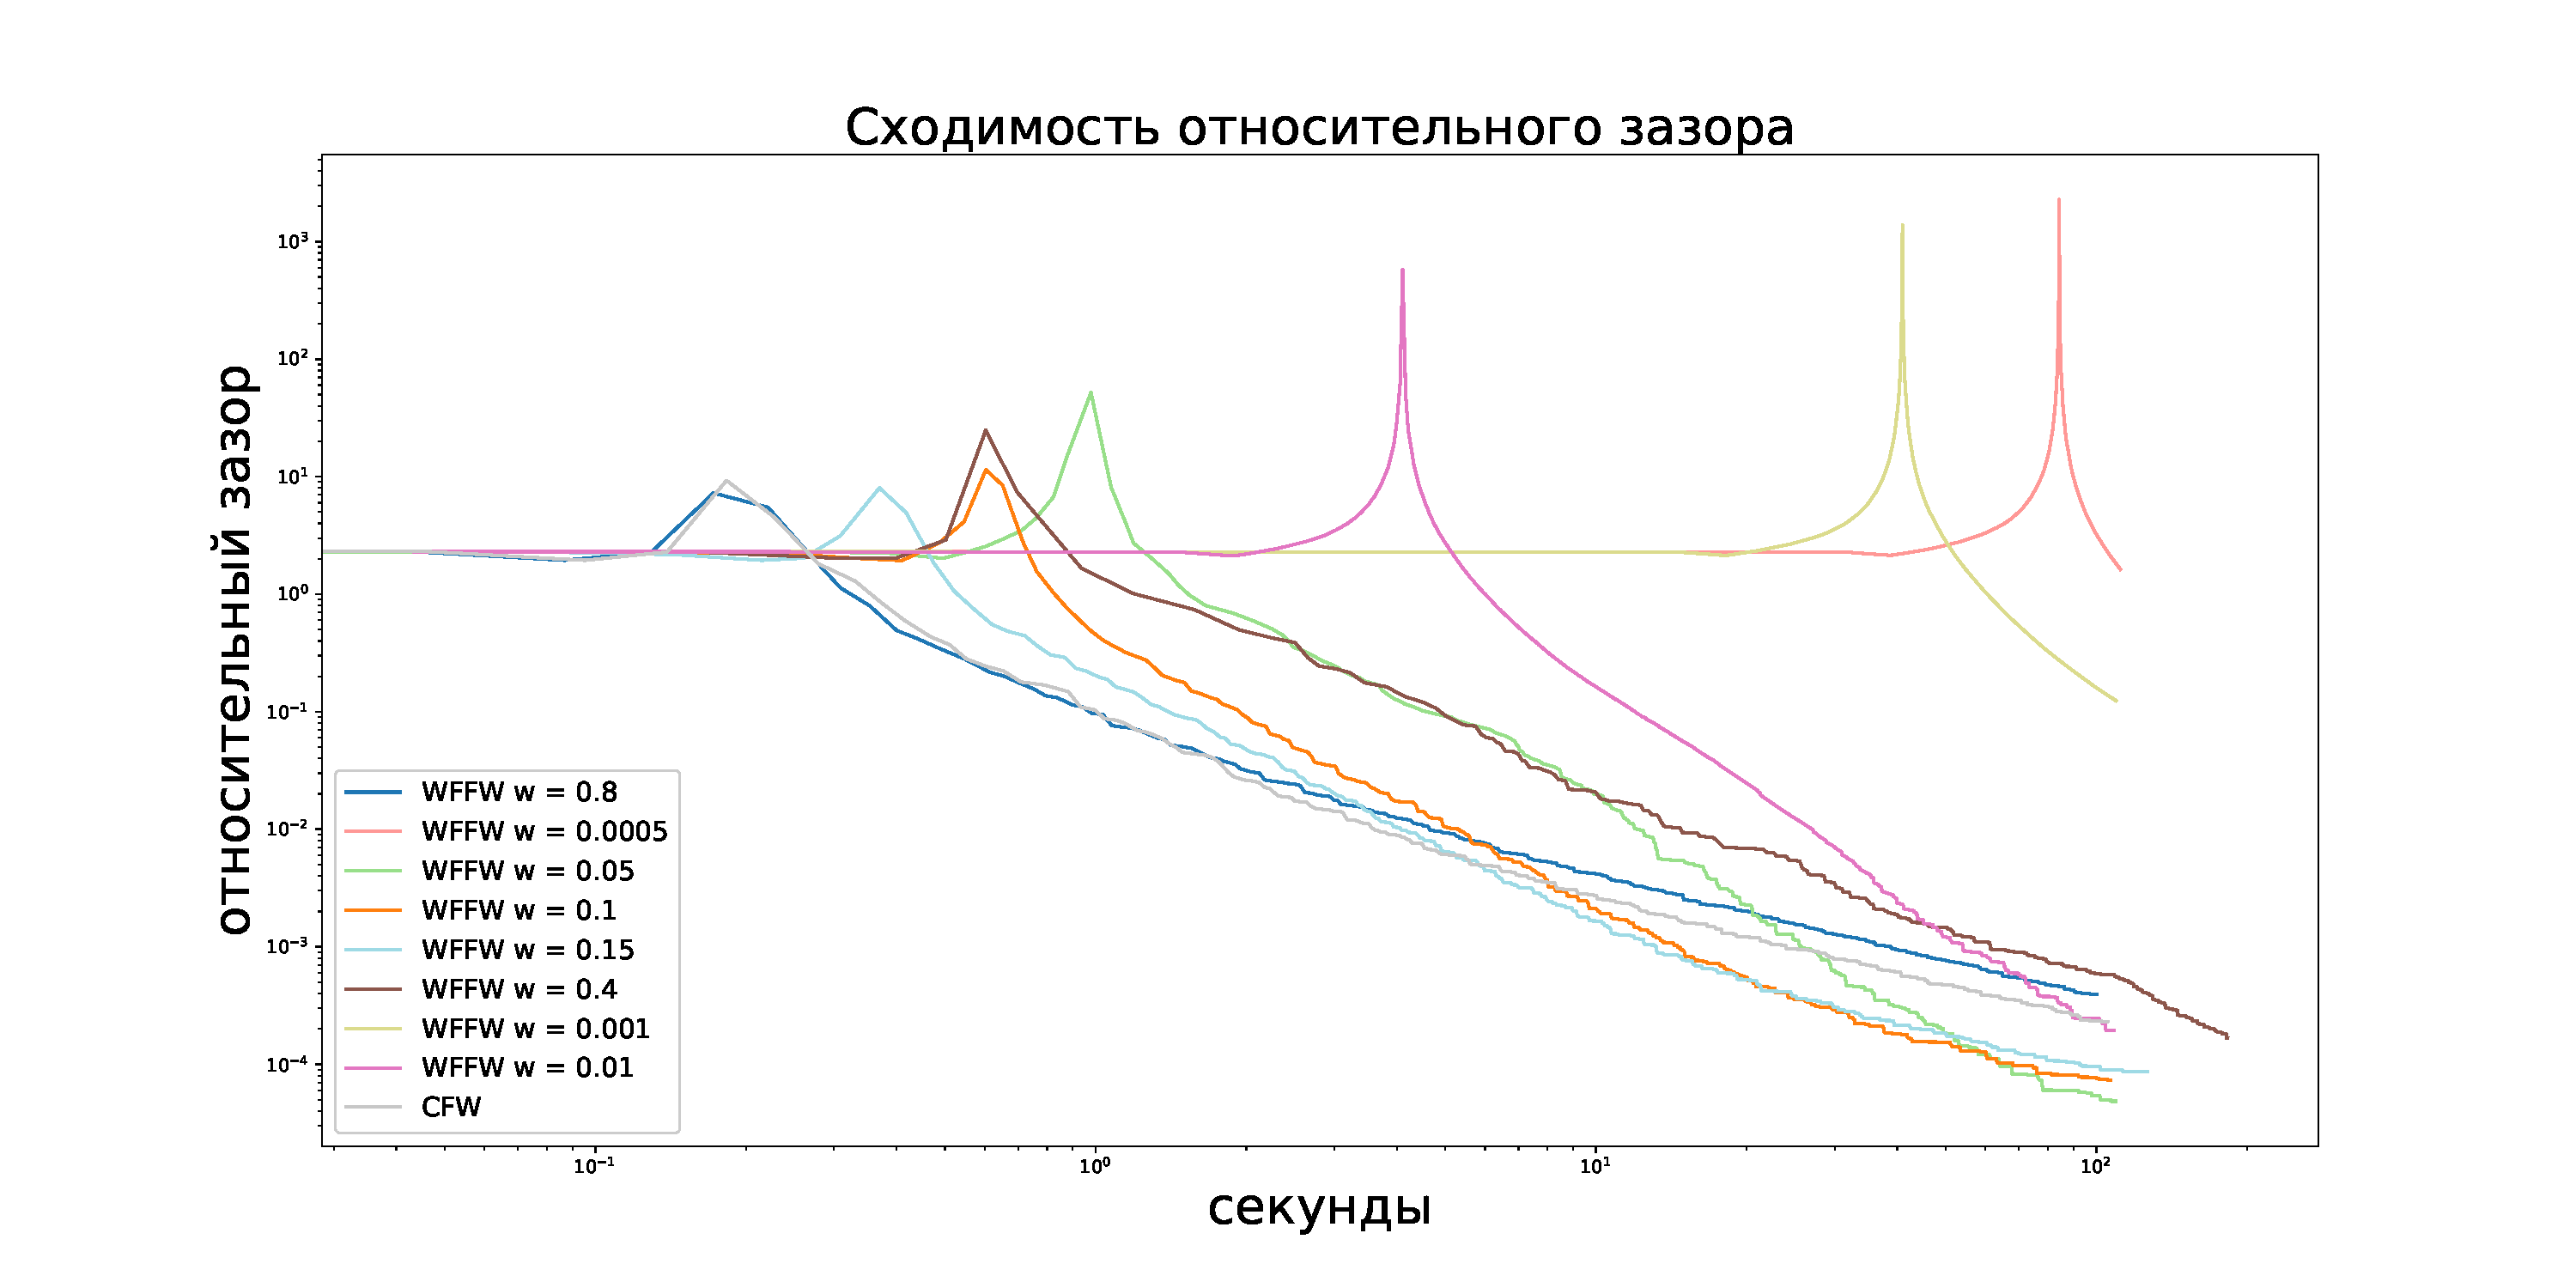
\includegraphics[width=0.98\textwidth]{fw_modifications/0_WFW.pdf}
\caption{Сходимость WFFW при различных параметрах геометрического сглаживания на сети Terrassa-Asymmetric.}
\label{fig:fw-mod-wffw-params}
\end{figure}

Основные наблюдения следующие.
Во-первых, методы, использующие предыдущие направления, в большинстве экспериментов сходятся
быстрее классического FW.
Во-вторых, использование более чем двух сопряженных направлений может давать дополнительное
ускорение: вариант $3$-conjugate FW часто оказывается одним из наиболее эффективных.
В-третьих, WFFW обычно улучшает FFW и CFW за счет управляемого забывания старых направлений,
хотя в ряде экспериментов уступает NFW.
Таким образом, использование памяти о предыдущих направлениях является устойчивым способом
ускорить FW без изменения линейного оракула.

\subsection{Одномерный поиск для BPR-функций}

Длина шага выбирается точной минимизацией
\[
    \gamma_k=\argmin_{\gamma\in[0,1]}\Psi(f^k+\gamma d^k).
\]
Для BPR-функции
\[
    \tau_e(f_e)=\bar t_e\left(1+\rho\left(\frac{f_e}{\bar f_e}\right)^{1/\mu}\right)
\]
производная одномерной функции равна
\[
    \frac{d}{d\gamma}\Psi(f^k+\gamma d^k)
    =
    \sum_{e\in\cE}
    \tau_e(f_e^k+\gamma d_e^k)d_e^k.
\]
Поэтому задача поиска $\gamma$ сводится к нахождению нуля монотонной функции на $[0,1]$.
Если производная в нуле неотрицательна, оптимум находится при $\gamma=0$.
Если производная в единице неположительна, оптимум находится при $\gamma=1$.
В остальных случаях используется одномерный численный метод.
Эта процедура одинакова для FW, CFW, BFW, FFW, WFFW и NFW; различается только направление
$d^k$.

\subsection{Итоги раздела}

Рассмотренное направление развития движется от уже известных CFW/BFW к двум новым вариантам.
NFW проверяет гипотезу, что память о большем числе прошлых направлений может усилить
эффект сопряженности.
WFFW проверяет другую гипотезу: может быть, часть ускорения объясняется не строгой
сопряженностью, а более устойчивым сглаживанием направлений.
Эксперименты показывают, что обе гипотезы полезны.
Сопряженные методы дают наиболее сильный эффект, но взвешенное сглаживание также улучшает
поведение классического FW.


\subsection{Выводы по модификациям}

Рассмотренные модификации сохраняют ключевое преимущество FW: каждая итерация требует решения той же линейной подзадачи, которая в транспортной модели сводится к поиску кратчайших путей.
Дополнительные вычисления связаны с линейным поиском и комбинированием предыдущих направлений.
Для модели Бекмана эти операции существенно дешевле линейного оракула, поскольку гессиан диагонален.

Эксперименты показывают, что направление шага является главным объектом для улучшения FW.
Наиболее перспективным оказывается семейство сопряженных методов, особенно NFW при малых значениях $N$.
Эта идея становится отправной точкой для следующей главы, где CFW и NFW переносятся из транспортной постановки в задачи машинного обучения.

\newpage

\section{Сопряженный Frank--Wolfe в задачах машинного обучения}
\label{sec:cfw-ml}

В этой главе модификации Frank--Wolfe с сопряженными направлениями переносятся из транспортной постановки в задачи машинного обучения.
Рассматривается гладкая выпуклая задача
\begin{equation}
    f(x)\to\min_{x\in\cX},
    \qquad
    f:\R^d\to\R,
    \label{eq:ml-constrained-problem}
\end{equation}
где $\cX$ является компактным выпуклым множеством.
Такая постановка возникает, например, когда регуляризованная задача машинного обучения переписывается как задача с ограничением на норму параметров.

Если исходная задача имеет вид
\[
    f(x)+\mu g(x)\to\min_x,
\]
то при подходящем выборе радиуса она может быть рассмотрена как
\[
    f(x)\to\min_{g(x)\leq R}.
\]
Для ограничений вида $\norm{x}_1\leq R$ линейный оракул Frank--Wolfe вычисляется проще, чем проекция на соответствующее множество.
Поэтому FW и его модификации естественно применимы к обучению моделей с ограничениями на параметры.

\subsection{Базовый FW для гладкой выпуклой задачи}

На итерации $k$ алгоритм решает линейную подзадачу
\begin{equation}
    s_k^{FW}
    =
    \argmin_{s\in\cX}
    \inner{\nabla f(x_k)}{s},
    \label{eq:ml-fw-lmo}
\end{equation}
после чего делает шаг
\[
    d_k=s_k^{FW}-x_k,
    \qquad
    x_{k+1}=x_k+\gamma_kd_k.
\]
Длина шага может задаваться теоретической последовательностью
\[
    \gamma_k=\frac{2}{k+2},
\]
или выбираться линейным поиском
\[
    \gamma_k=
    \argmin_{\gamma\in[0,1]}
    f(x_k+\gamma d_k).
\]

\begin{algorithm}
\caption{Frank--Wolfe для задачи машинного обучения}
\begin{algorithmic}
\REQUIRE компактное выпуклое множество $\cX$, начальная точка $x_0\in\cX$
\STATE $k\gets 0$
\REPEAT
\STATE $s_k^{FW}\gets\argmin_{s\in\cX}\inner{\nabla f(x_k)}{s}$
\STATE $d_k\gets s_k^{FW}-x_k$
\STATE $\gamma_k\gets\argmin_{\gamma\in[0,1]}f(x_k+\gamma d_k)$
\STATE $x_{k+1}\gets x_k+\gamma_kd_k$
\STATE $k\gets k+1$
\UNTIL{достигнут критерий остановки}
\end{algorithmic}
\end{algorithm}

\subsection{CFW без явного вычисления гессиана}

В транспортной задаче гессиан модели Бекмана диагонален, поэтому вычисление коэффициента CFW по формуле~\eqref{eq:cfw-alpha-traffic} дешево.
В задачах машинного обучения явное вычисление гессиана может быть слишком дорогим.
Поэтому используется приближение произведения гессиана на вектор через разность градиентов.

Пусть
\[
    d_{k-1}=s_{k-1}-x_{k-1},
    \qquad
    x_k=x_{k-1}+\gamma_{k-1}d_{k-1}.
\]
Тогда
\[
    s_{k-1}-x_{k-1}
    =
    \frac{x_k-x_{k-1}}{\gamma_{k-1}},
\]
и произведение гессиана на предыдущее направление приближенно выражается как
\[
    \nabla^2 f(x_k)(s_{k-1}-x_{k-1})
    \approx
    \frac{\nabla f(x_k)-\nabla f(x_{k-1})}{\gamma_{k-1}}.
\]
После сокращения $\gamma_{k-1}$ получается формула
\begin{equation}
    \alpha =
    \frac{
        (x_k-s_{k-1})^T(\nabla f(x_k)-\nabla f(x_{k-1}))
    }{
        (s_k^{FW}-s_{k-1})^T(\nabla f(x_k)-\nabla f(x_{k-1}))
    }.
    \label{eq:cfw-alpha-grad-diff}
\end{equation}
Эта формула не требует явного построения гессиана и хорошо согласуется с реализацией в библиотеках автоматического дифференцирования.

\begin{algorithm}
\caption{Conjugate Frank--Wolfe для общей гладкой задачи}
\begin{algorithmic}
\REQUIRE $x_0\in\cX$, параметр $\alpha_0\in(0,1]$
\STATE выполнить один шаг FW и получить $x_1$, $s_0$
\STATE $k\gets 1$
\REPEAT
\STATE $s_k^{FW}\gets\argmin_{s\in\cX}\inner{\nabla f(x_k)}{s}$
\IF{$\inner{\nabla f(x_k)}{s_k^{FW}}=\inner{\nabla f(x_k)}{x_k}$}
\STATE остановить алгоритм
\ENDIF
\STATE вычислить $\alpha$ по формуле~\eqref{eq:cfw-alpha-grad-diff}
\STATE $\alpha\gets\min\{1,\max\{\alpha_0,\alpha\}\}$
\STATE $s_k\gets\alpha s_k^{FW}+(1-\alpha)s_{k-1}$
\STATE $d_k\gets s_k-x_k$
\STATE $\gamma_k\gets\argmin_{\gamma\in[0,1]}f(x_k+\gamma d_k)$
\STATE $x_{k+1}\gets x_k+\gamma_kd_k$
\STATE $k\gets k+1$
\UNTIL{достигнут критерий остановки}
\end{algorithmic}
\end{algorithm}

\subsection{Сходимость CFW}

Для анализа используется стандартное предположение о выпуклости и гладкости.

\begin{assumption}
\label{ass:ml-smooth}
Множество $\cX\subset\R^d$ выпукло и компактно.
Функция $f:\R^d\to\R$ выпукла и непрерывно дифференцируема, а ее градиент липшицев на $\cX$ с константой $L$:
\[
    0
    \leq
    f(x')-f(x)-\inner{\nabla f(x)}{x'-x}
    \leq
    \frac{L}{2}\norm{x'-x}_2^2,
    \qquad
    x,x'\in\cX.
\]
\end{assumption}

Зазор Frank--Wolfe в точке $x_k$ равен
\[
    g_k=
    \inner{\nabla f(x_k)}{x_k-s_k^{FW}}.
\]
Обозначим
\[
    h_0=f(x_0)-f(x^\ast),
    \qquad
    R=\Max_{x,y\in\cX}\norm{x-y}_2,
    \qquad
    A=LR^2.
\]

\begin{lemma}
\label{lem:cfw-descent-direction}
Пусть $d_k$ является направлением шага CFW, а длина шага выбирается точным линейным поиском на отрезке $[0,1]$.
Тогда
\[
    \inner{\nabla f(x_{k+1})}{d_k}\leq 0.
\]
\end{lemma}

\begin{proof}
Докажем утверждение по индукции.
На нулевой итерации направление CFW совпадает с направлением FW:
\[
    d_0=d_0^{FW}=s_0^{FW}-x_0.
\]
Рассмотрим одномерную функцию
\[
    \varphi(\gamma)=f(x_0+\gamma d_0)
\]
на отрезке $[0,1]$.
Если $x_0$ не является решением, то по условию оптимальности для выпуклой задачи
\[
    \varphi'(0)=
    \inner{\nabla f(x_0)}{s_0^{FW}-x_0}<0.
\]
Следовательно, точный линейный поиск выбирает $\gamma_0>0$.
Так как $\varphi$ выпукла, условие оптимальности одномерной задачи
\[
    \gamma_0\in\argmin_{\gamma\in[0,1]}\varphi(\gamma)
\]
дает
\[
    \varphi'(\gamma_0)\leq 0,
    \qquad
    \inner{\nabla f(x_1)}{d_0}\leq 0.
\]
Если же $x_0$ уже является решением, алгоритм останавливается, и утверждение не требуется.

Пусть теперь для предыдущей итерации выполнено
\[
    \inner{\nabla f(x_k)}{d_{k-1}}\leq 0.
\]
Для направления CFW имеем
\[
    d_k
    =
    \alpha d_k^{FW}
    +
    (1-\alpha)(s_{k-1}-x_k)
    =
    \alpha d_k^{FW}
    +
    (1-\alpha)(1-\gamma_{k-1})d_{k-1}.
\]
Здесь $\alpha\in[\alpha_0,1]$.
По определению линейного оракула
\[
    \inner{\nabla f(x_k)}{d_k^{FW}}
    =
    \inner{\nabla f(x_k)}{s_k^{FW}-x_k}
    =
    -g_k\leq 0,
\]
а второе слагаемое не положительно по предположению индукции.
Значит,
\[
    \inner{\nabla f(x_k)}{d_k}
    \leq 0.
\]
Если $g_k>0$, то производная одномерной функции
\[
    \varphi_k(\gamma)=f(x_k+\gamma d_k)
\]
в нуле отрицательна или равна нулю только в вырожденном случае.
Точный линейный поиск по выпуклой функции снова дает
\[
    \inner{\nabla f(x_{k+1})}{d_k}
    =
    \varphi_k'(\gamma_k)
    \leq 0.
\]
Тем самым индукция завершена.
\end{proof}

\begin{theorem}
\label{thm:cfw-rate}
Пусть выполнено предположение~\ref{ass:ml-smooth}.
Тогда для CFW с параметром $\alpha_0\in(0,1]$ справедлива оценка
\[
    g_N^\ast
    =
    \Min_{1\leq k\leq N}g_k
    \leq
    \frac{\max\{2h_0,A\}}{\alpha_0\sqrt{N+1}}.
\]
\end{theorem}

\begin{proof}
Так как $\gamma_k$ выбирается точным линейным поиском, для любого $\gamma\in[0,1]$
выполнено
\[
    f(x_{k+1})
    =
    \min_{\eta\in[0,1]}f(x_k+\eta d_k)
    \leq
    f(x_k+\gamma d_k).
\]
Используя $L$-гладкость, получаем
\[
    f(x_{k+1})
    \leq
    f(x_k)
    +
    \gamma\inner{\nabla f(x_k)}{d_k}
    +
    \frac{\gamma^2L}{2}\norm{d_k}_2^2.
\]
Далее
\[
    d_k
    =
    \alpha_k d_k^{FW}
    +
    (1-\alpha_k)(1-\gamma_{k-1})d_{k-1}.
\]
По лемме~\ref{lem:cfw-descent-direction}, примененной к предыдущему шагу,
\[
    \inner{\nabla f(x_k)}{d_{k-1}}\leq 0.
\]
Следовательно,
\[
    \inner{\nabla f(x_k)}{d_k}
    \leq
    \alpha_k\inner{\nabla f(x_k)}{d_k^{FW}}
    =
    -\alpha_k g_k
    \leq
    -\alpha_0 g_k.
\]
Так как $x_k,s_k\in\cX$ и $R$ является диаметром $\cX$,
\[
    \norm{d_k}_2\leq R,
    \qquad
    A=LR^2.
\]
Следовательно,
\[
    f(x_{k+1})
    \leq
    f(x_k)
    +
    \Min_{\gamma\in[0,1]}
    \left\{
        -\alpha_0\gamma g_k
        +
        \frac{\gamma^2A}{2}
    \right\}.
\]
Минимум в правой части достигается либо во внутренней точке,
либо на правой границе отрезка.
Поэтому
\[
    f(x_{k+1})-f(x_k)
    \leq
    -\frac{\alpha_0g_k}{2}
    \min\left\{
        \frac{\alpha_0g_k}{A},
        1
    \right\}.
\]
Суммируя по $k=0,\ldots,N$ и используя $f(x^\ast)\leq f(x_{N+1})$, получаем
\[
    h_0
    \geq
    \sum_{k=0}^{N}
    \frac{\alpha_0g_k}{2}
    \min\left\{
        \frac{\alpha_0g_k}{A},
        1
    \right\}.
\]
Так как $g_N^\ast=\min_{0\leq k\leq N}g_k$, то
\[
    h_0
    \geq
    (N+1)
    \frac{\alpha_0g_N^\ast}{2}
    \min\left\{
        \frac{\alpha_0g_N^\ast}{A},
        1
    \right\}.
\]
Если $\alpha_0g_N^\ast\leq A$, то
\[
    \alpha_0g_N^\ast
    \leq
    \sqrt{\frac{2Ah_0}{N+1}}
    \leq
    \frac{\max\{2h_0,A\}}{\sqrt{N+1}}.
\]
Если $\alpha_0g_N^\ast>A$, то
\[
    \alpha_0g_N^\ast
    \leq
    \frac{2h_0}{N+1}
    \leq
    \frac{\max\{2h_0,A\}}{\sqrt{N+1}}.
\]
Объединяя два случая, получаем утверждение теоремы.
\end{proof}

Оценка отличается от стандартной оценки FW только множителем $1/\alpha_0$.
Это означает, что CFW сохраняет асимптотический порядок сходимости FW по зазору Frank--Wolfe, а практическое ускорение связано с более удачным выбором направления.

\subsection{NFW в машинном обучении}

Метод Bi-conjugate Frank--Wolfe обобщается до N-conjugate Frank--Wolfe, где новое
направление строится с учетом нескольких предыдущих направлений.
Предполагается, что предыдущие направления сопряжены между собой относительно нового
гессиана:
\[
    d_{k-m}^T\nabla^2f(x_k)d_{k-n}=0,
    \qquad
    m\neq n,\quad m,n\in\{1,\ldots,N\}.
\]
Новая точка направления записывается как выпуклая комбинация текущей точки линейного
оракула и нескольких предыдущих точек:
\[
    s_k
    =
    \alpha_0s_k^{FW}
    +
    \sum_{m=1}^{N}\alpha_ms_{k-m}.
\]
Коэффициенты выбираются так, чтобы новое направление было сопряжено с предыдущими:
\[
    d_{k-m}^T\nabla^2f(x_k)d_k=0,
    \qquad m=1,\ldots,N.
\]

Обозначим $H^k=\nabla^2f(x_k)$ и
\[
    A_{k-m}=d_{k-m}^TH^kd_k^{FW},
    \qquad
    B_{k-m}=d_{k-m}^TH^kd_{k-m}.
\]
Если на текущей итерации используется $N_{\mathrm{curr}}$ предыдущих направлений, то
сначала вычисляется
\[
    \beta_{N_{\mathrm{curr}}}
    =
    \frac{-A_{k-N_{\mathrm{curr}}}}
    {B_{k-N_{\mathrm{curr}}}(1-\gamma_{k-N_{\mathrm{curr}}})},
\]
а затем последовательно для $m=N_{\mathrm{curr}}-1,\ldots,1$:
\[
    \beta_m
    =
    \frac{-A_{k-m}}{B_{k-m}(1-\gamma_{k-m})}
    +
    \frac{\gamma_{k-m}}{1-\gamma_{k-m}}
    \sum_{n=m+1}^{N_{\mathrm{curr}}}\beta_n.
\]
После этого
\[
    \alpha_m=\beta_m\alpha_0,
    \qquad
    \alpha_0=
    \frac{1}{1+\sum_{i=1}^{N_{\mathrm{curr}}}\beta_i}.
\]

Для ML-задач точное вычисление $H^k$ обычно слишком дорого.
Поэтому, как и в CFW, используется приближение произведений гессиана через разности
градиентов.
Для предыдущего направления $d_{k-m}=s_{k-m}-x_{k-m}$ применяется оценка
\[
    \nabla f(s_{k-m})-\nabla f(x_{k-m})
    \approx
    \nabla^2f(x_{k-m})(s_{k-m}-x_{k-m}).
\]
Если гессиан за несколько итераций меняется умеренно, то отношение, входящее в формулы
для коэффициентов, можно заменить выражением
\[
    \frac{A_{k-m}}{B_{k-m}}
    \approx
    \frac{
        (\nabla f(s_{k-m})-\nabla f(x_{k-m}))^Td_k^{FW}
    }{
        (\nabla f(s_{k-m})-\nabla f(x_{k-m}))^T(s_{k-m}-x_{k-m})
    }.
\]
Так NFW сохраняет идею сопряжения с несколькими предыдущими направлениями, но не требует
явного построения матрицы Гессе.

\begin{algorithm}
\caption{N-conjugate Frank--Wolfe для задачи машинного обучения}
\label{alg:nfw-ml}
\begin{algorithmic}
\REQUIRE начальная точка $x_0\in\cX$, глубина памяти $N$, параметр $\gamma_{\max}\in[0,1]$
\STATE выполнить начальный FW-шаг и получить $x_1$, $s_0$, $N_{\mathrm{curr}}\gets 1$
\REPEAT
\STATE $s_k^{FW}\gets\argmin_{s\in\cX}\inner{\nabla f(x_k)}{s}$
\STATE вычислить коэффициенты $\alpha_0,\ldots,\alpha_{N_{\mathrm{curr}}}$
\STATE $s_k\gets\alpha_0s_k^{FW}+\sum_{i=1}^{N_{\mathrm{curr}}}\alpha_is_{k-i}$
\STATE $d_k\gets s_k-x_k$
\STATE $\gamma_k\gets\argmin_{\gamma\in[0,1]}f(x_k+\gamma d_k)$
\STATE $x_{k+1}\gets x_k+\gamma_kd_k$
\STATE обновить $N_{\mathrm{curr}}$: увеличить до $N$ или сбросить до $1$, если $\gamma_k>\gamma_{\max}$
\UNTIL{достигнут критерий остановки}
\end{algorithmic}
\end{algorithm}

\subsection{Эксперименты на логистической регрессии}

Эксперименты проводились на задачах бинарной классификации с логистической регрессией на наборах Mushrooms и MNIST.
Рассматривалась задача
\[
    \norm{w}_1\leq R,
\]
а также вариант с $l_2$-регуляризацией:
\[
    f(w)=\operatorname{logloss}(w)+\frac{\lambda}{2}\norm{w}_2^2.
\]
Интерес представляло сравнение случаев, когда решение безусловной задачи лежит внутри допустимого множества, около границы или далеко вне него.

\begin{table}[H]
\centering
\caption{$l_1$-нормы решений безусловной задачи для разных датасетов и регуляризаций.}
\begin{tabular}{lcc}
\toprule
Датасет & Без регуляризации & $l_2$-регуляризация \\
\midrule
Mushrooms & $>1000$ & $30.5$ \\
MNIST & $2.77$ & $0.15$ \\
\bottomrule
\end{tabular}
\label{tab:cfw-ml-l1-norms}
\end{table}

\noindent\textbf{Частота настоящей сопряженности.}
Так как коэффициент $\alpha$ в CFW проецируется на $[\alpha_0,1]$, важно понять,
как часто алгоритм действительно строит сопряженное направление, а не просто использует
усеченный коэффициент.
Направление считается сопряженным в этом смысле, если неусеченное значение $\alpha$ уже
лежит в отрезке $[\alpha_0,1]$.
Для численной проверки использовалась нормированная величина сопряженности
\[
    \eta_k
    =
    \frac{
        \left|d_{k-1}^T\nabla^2 f(x_k)d_k\right|
    }{
        \sqrt{
            \left(d_{k-1}^T\nabla^2 f(x_k)d_{k-1}\right)
            \left(d_k^T\nabla^2 f(x_k)d_k\right)
        }
    }.
\]
В точной арифметике для сопряженных направлений $\eta_k=0$.
Нормировка нужна, чтобы сравнивать значения на разных итерациях независимо от масштаба
направлений.
На рис.~\ref{fig:cfw-ml-conjugacy-frequency} показано значение $\eta_k$ на первых ста
итерациях CFW.
В эксперименте примерно в $80\%$ итераций новое направление действительно оказывается
сопряженным с предыдущим; при этом на начальных итерациях такие направления встречаются
реже.

\begin{figure}[H]
\centering
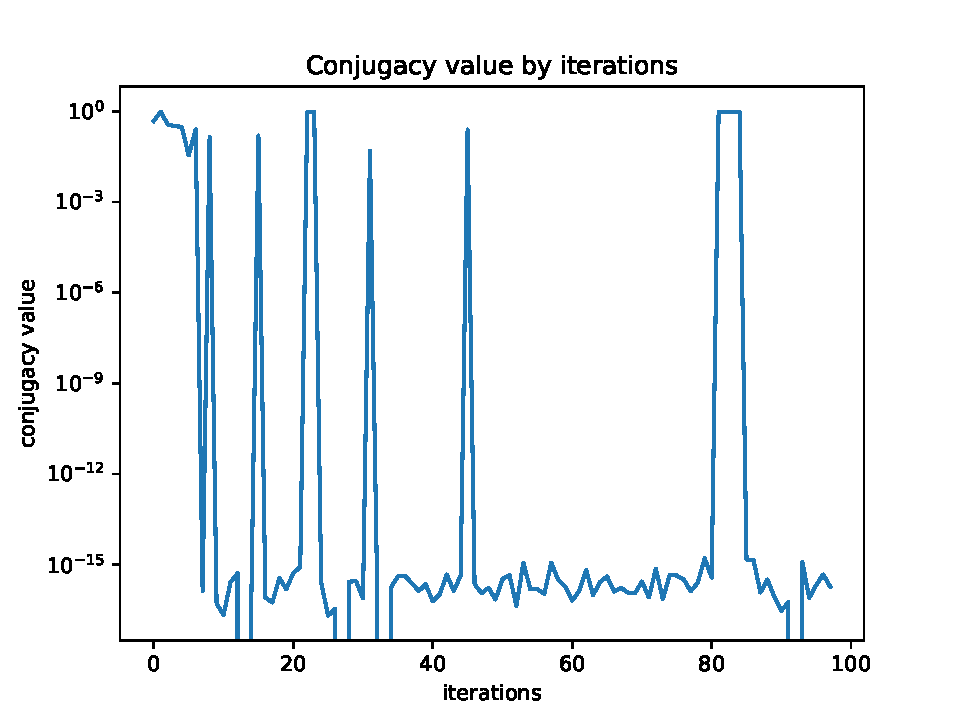
\includegraphics[width=0.72\textwidth]{cfw_ml/Experiment_3_fig_1.pdf}
\caption{Частота настоящей сопряженности на первых 100 итерациях CFW.}
\label{fig:cfw-ml-conjugacy-frequency}
\end{figure}

\noindent\textbf{Сравнение модификаций.}
Сравнивались FW с линейным поиском, FW с теоретическим шагом, CFW и NFW при $N=2,3,4,5$.
Во всех экспериментах для CFW использовалось $\alpha_0=0.05$.
Критерием качества был зазор Frank--Wolfe.

На рис.~\ref{fig:cfw-ml-mushrooms-12}--\ref{fig:cfw-ml-mnist-l2-34} приведены графики
сходимости для четырех групп задач: Mushrooms без регуляризации, Mushrooms с
$l_2$-регуляризацией, MNIST без регуляризации и MNIST с $l_2$-регуляризацией.
Для каждого датасета рассматриваются разные радиусы ограничения $\norm{w}_1\leq R$.

\begin{figure}[H]
\centering
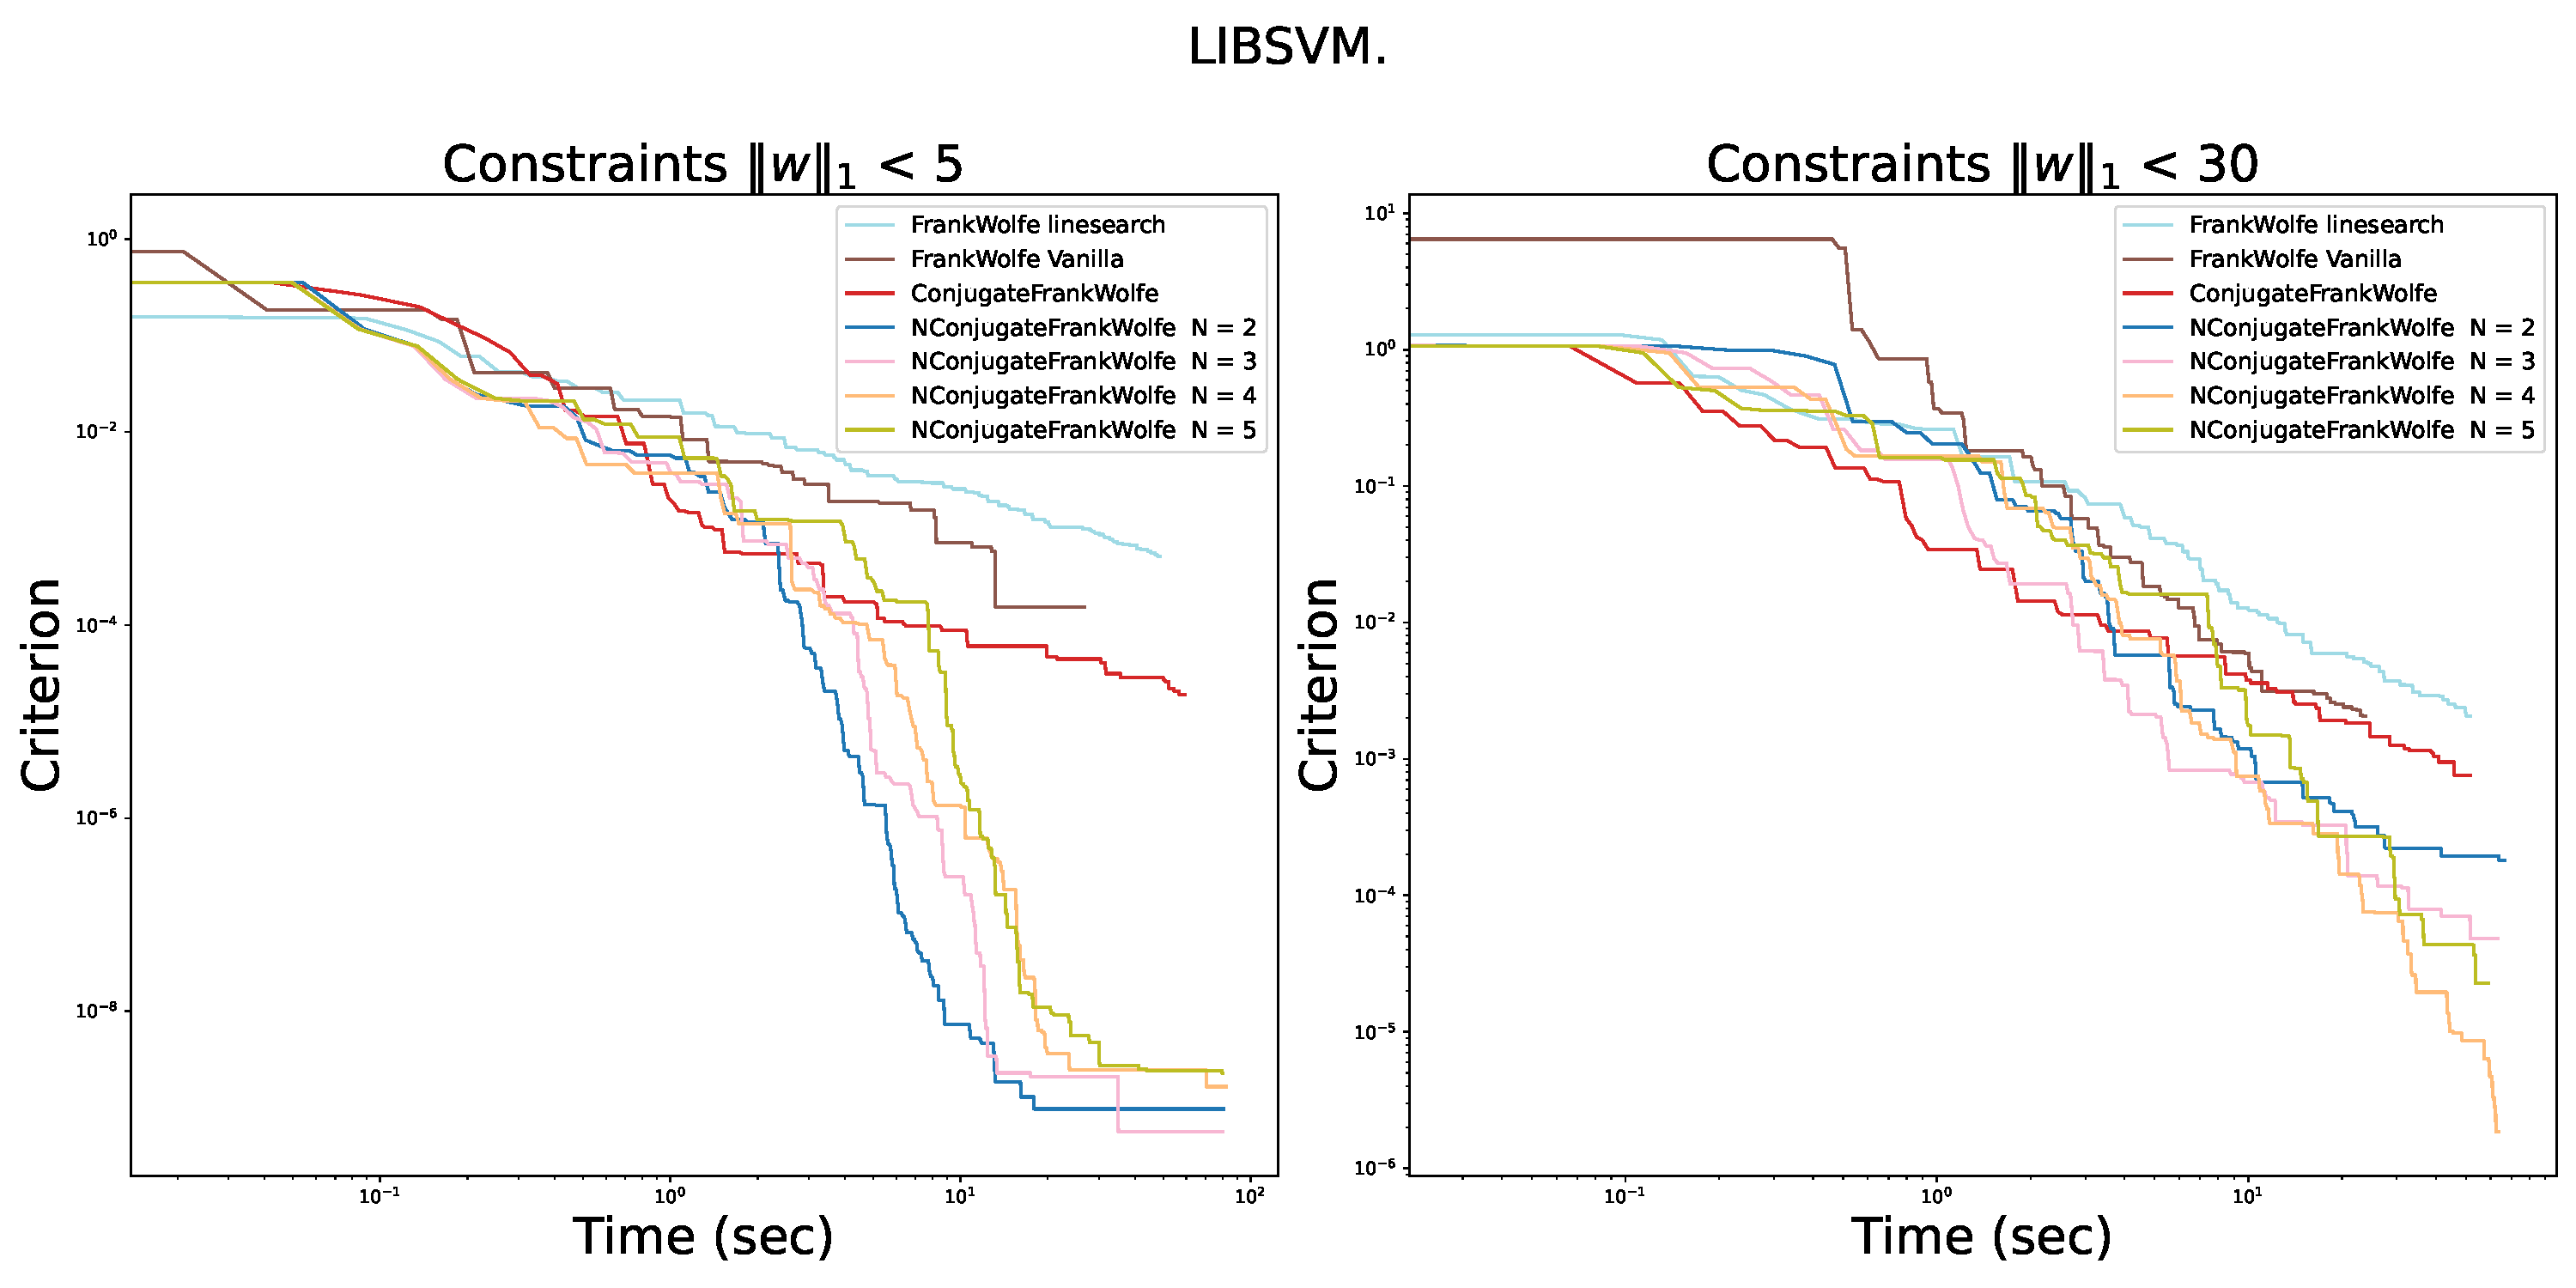
\includegraphics[width=0.96\textwidth]{cfw_ml/Experiment_5_fig_12.pdf}
\caption{Mushrooms без $l_2$-регуляризации: сходимость FW, CFW и NFW по FW-зазору для первых значений радиуса $R$.}
\label{fig:cfw-ml-mushrooms-12}
\end{figure}

\begin{figure}[H]
\centering
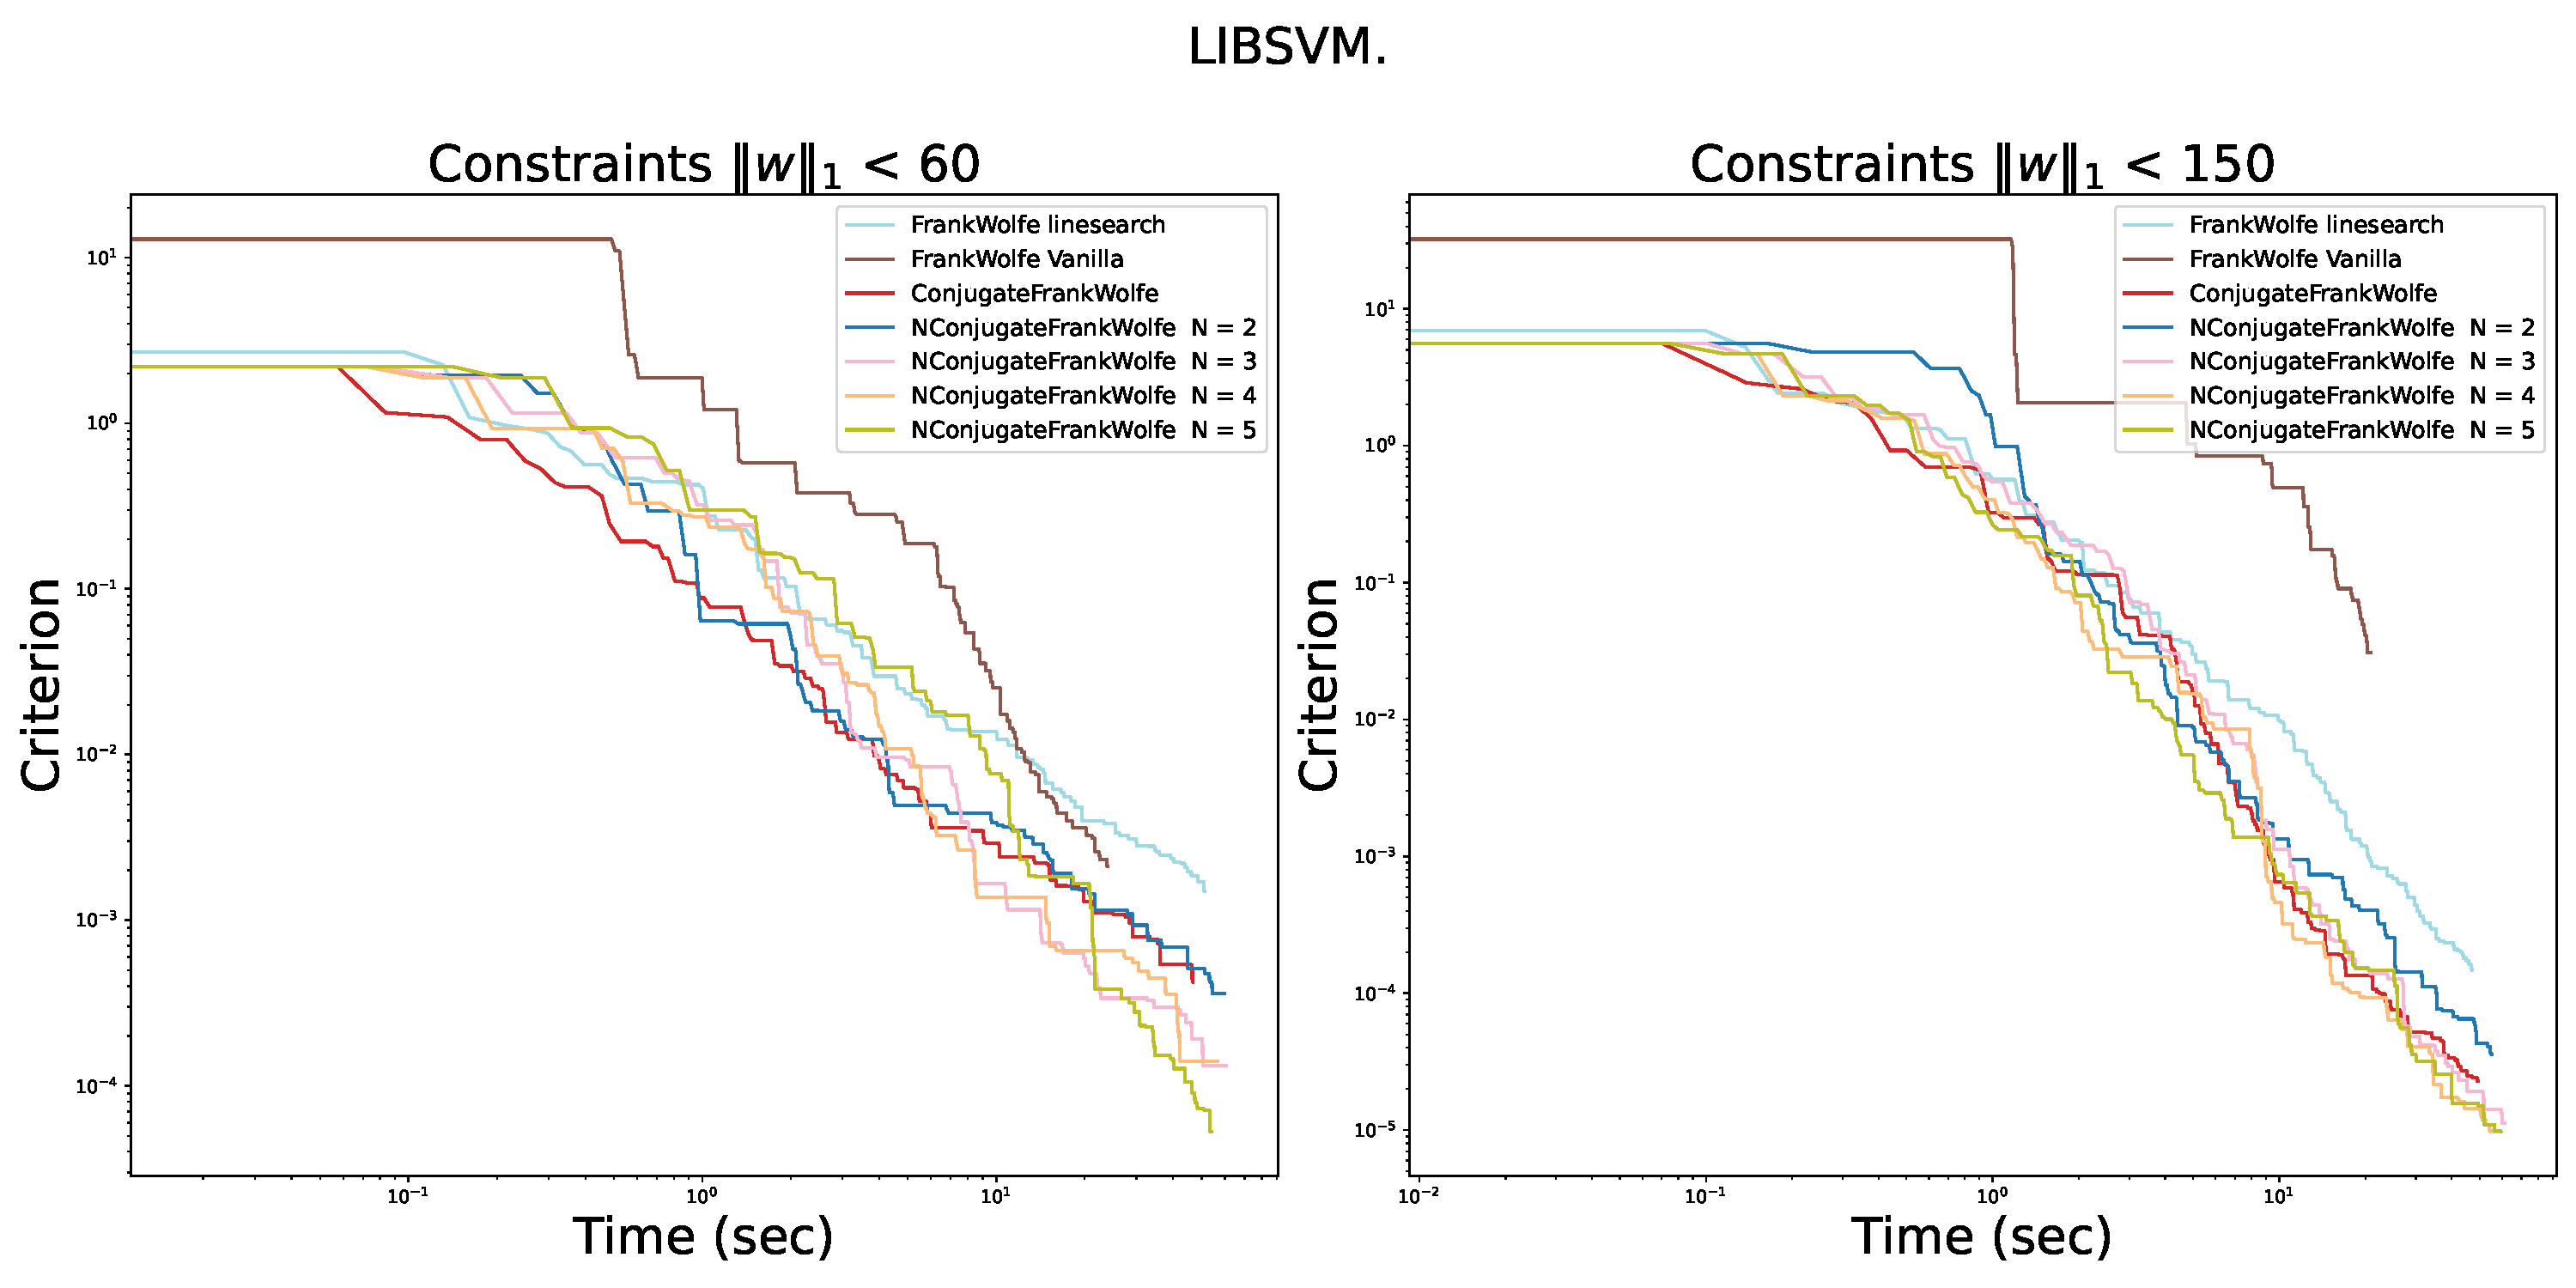
\includegraphics[width=0.96\textwidth]{cfw_ml/Experiment_5_fig_34.pdf}
\caption{Mushrooms без $l_2$-регуляризации: сходимость FW, CFW и NFW по FW-зазору для больших значений радиуса $R$.}
\label{fig:cfw-ml-mushrooms-34}
\end{figure}

\begin{figure}[H]
\centering
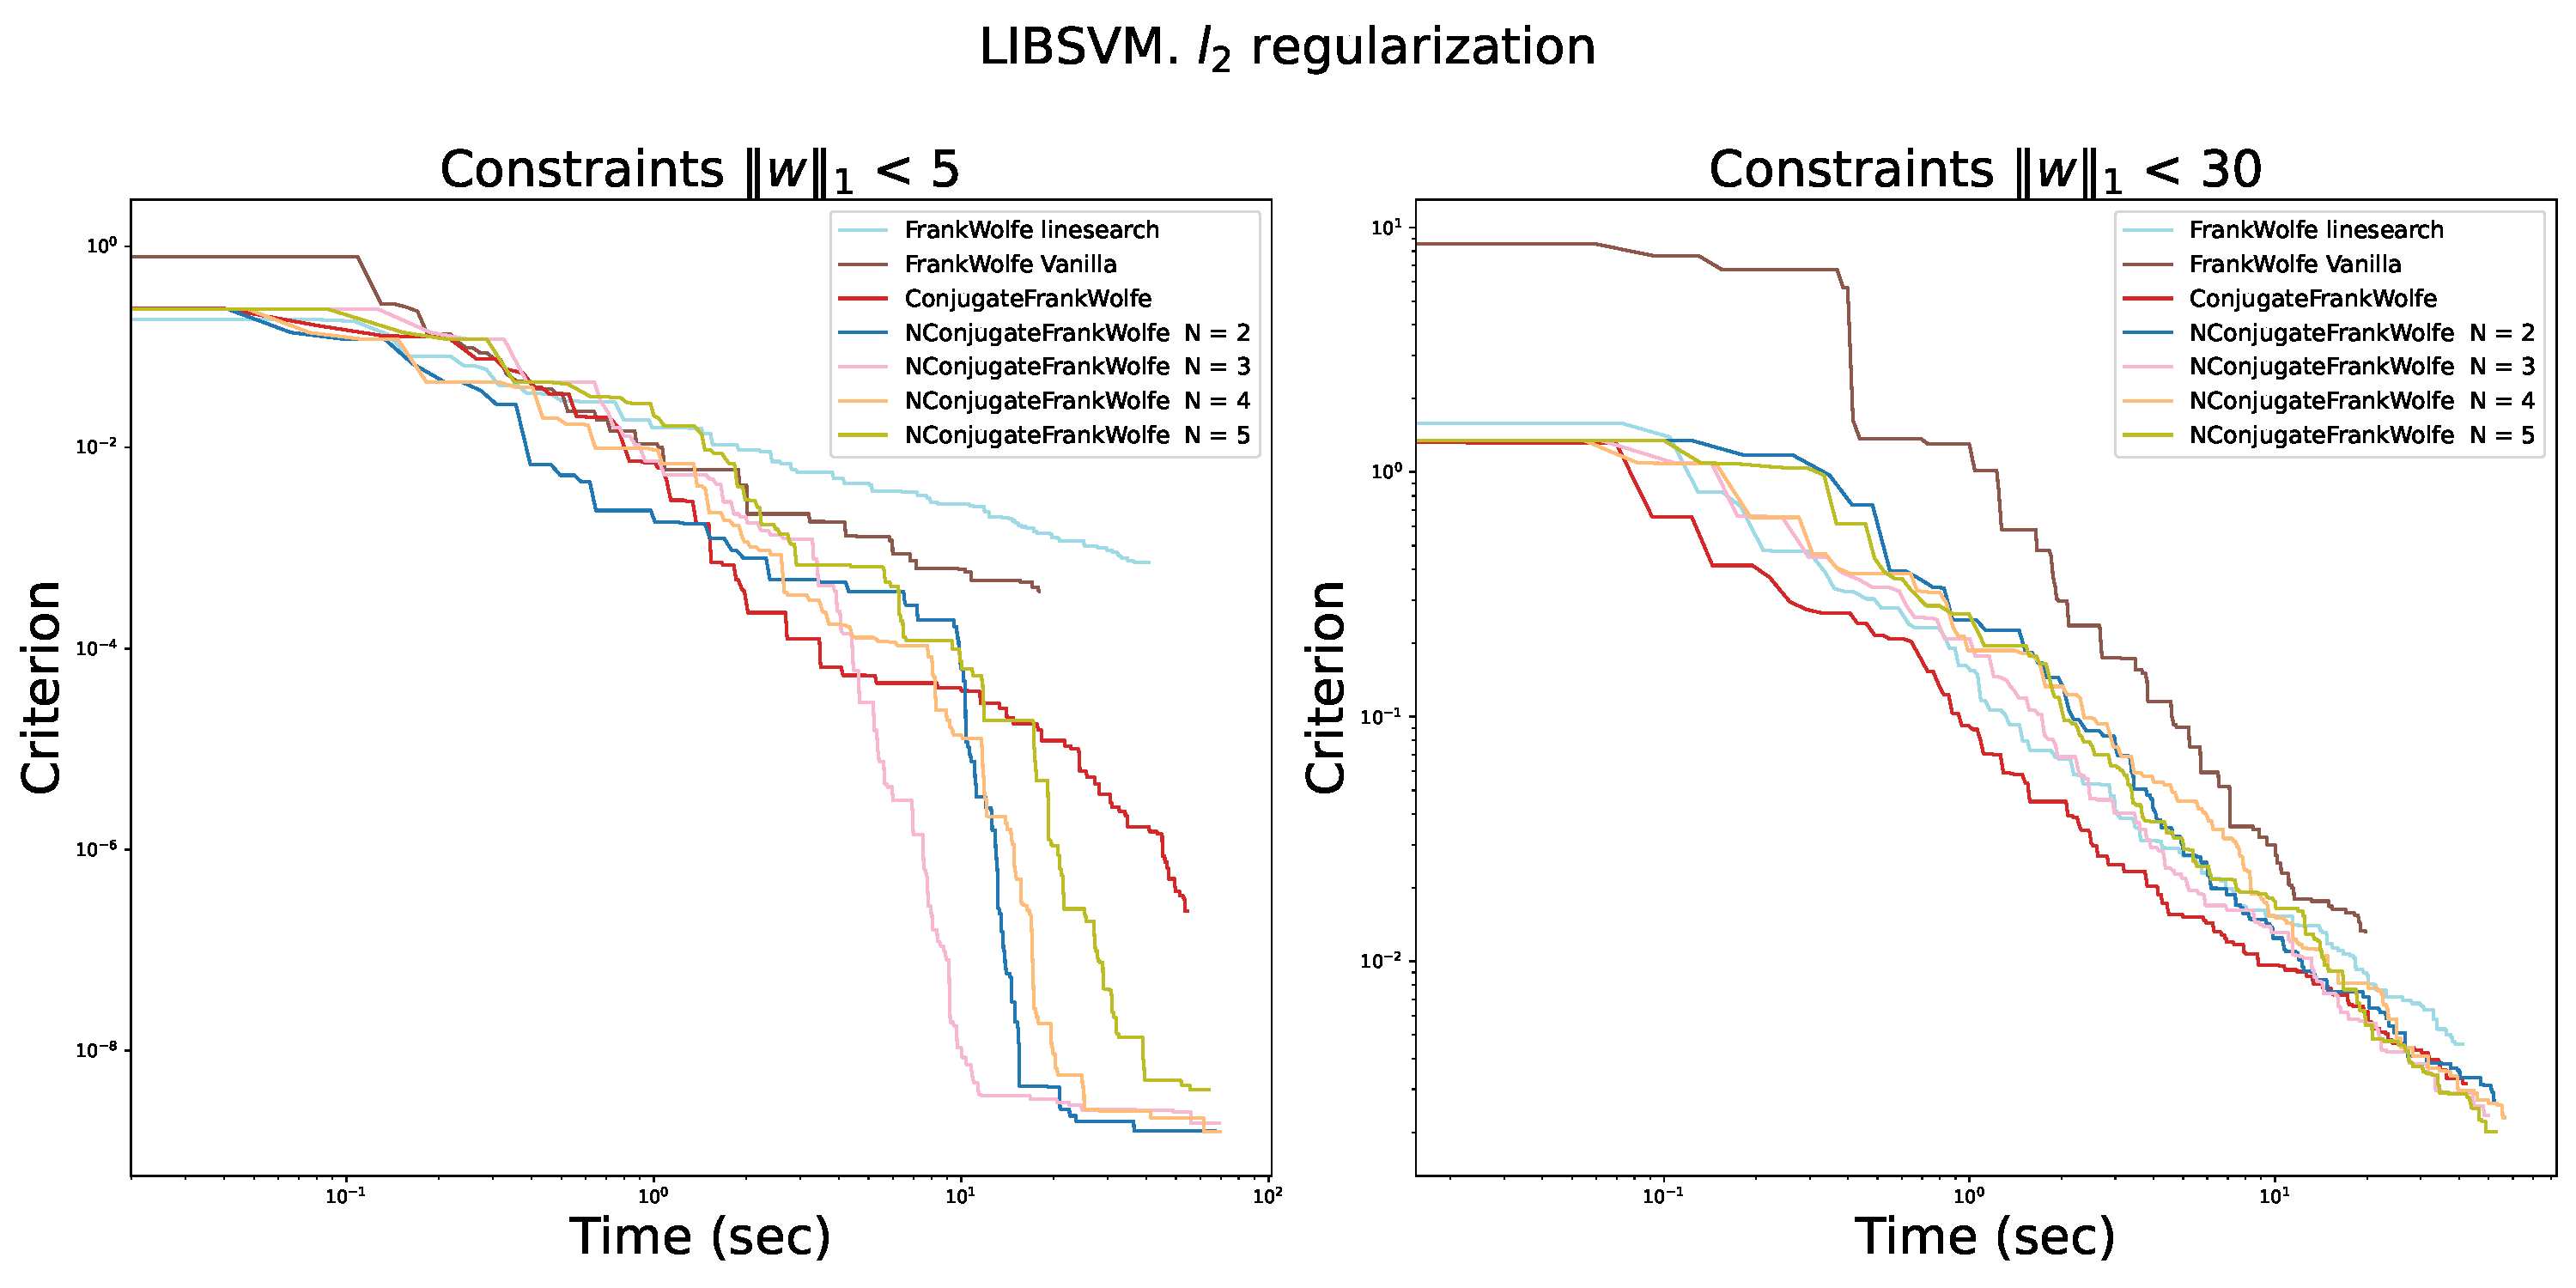
\includegraphics[width=0.96\textwidth]{cfw_ml/Experiment_6_fig_12.pdf}
\caption{Mushrooms с $l_2$-регуляризацией: сходимость FW, CFW и NFW по FW-зазору для первых значений радиуса $R$.}
\label{fig:cfw-ml-mushrooms-l2-12}
\end{figure}

\begin{figure}[H]
\centering
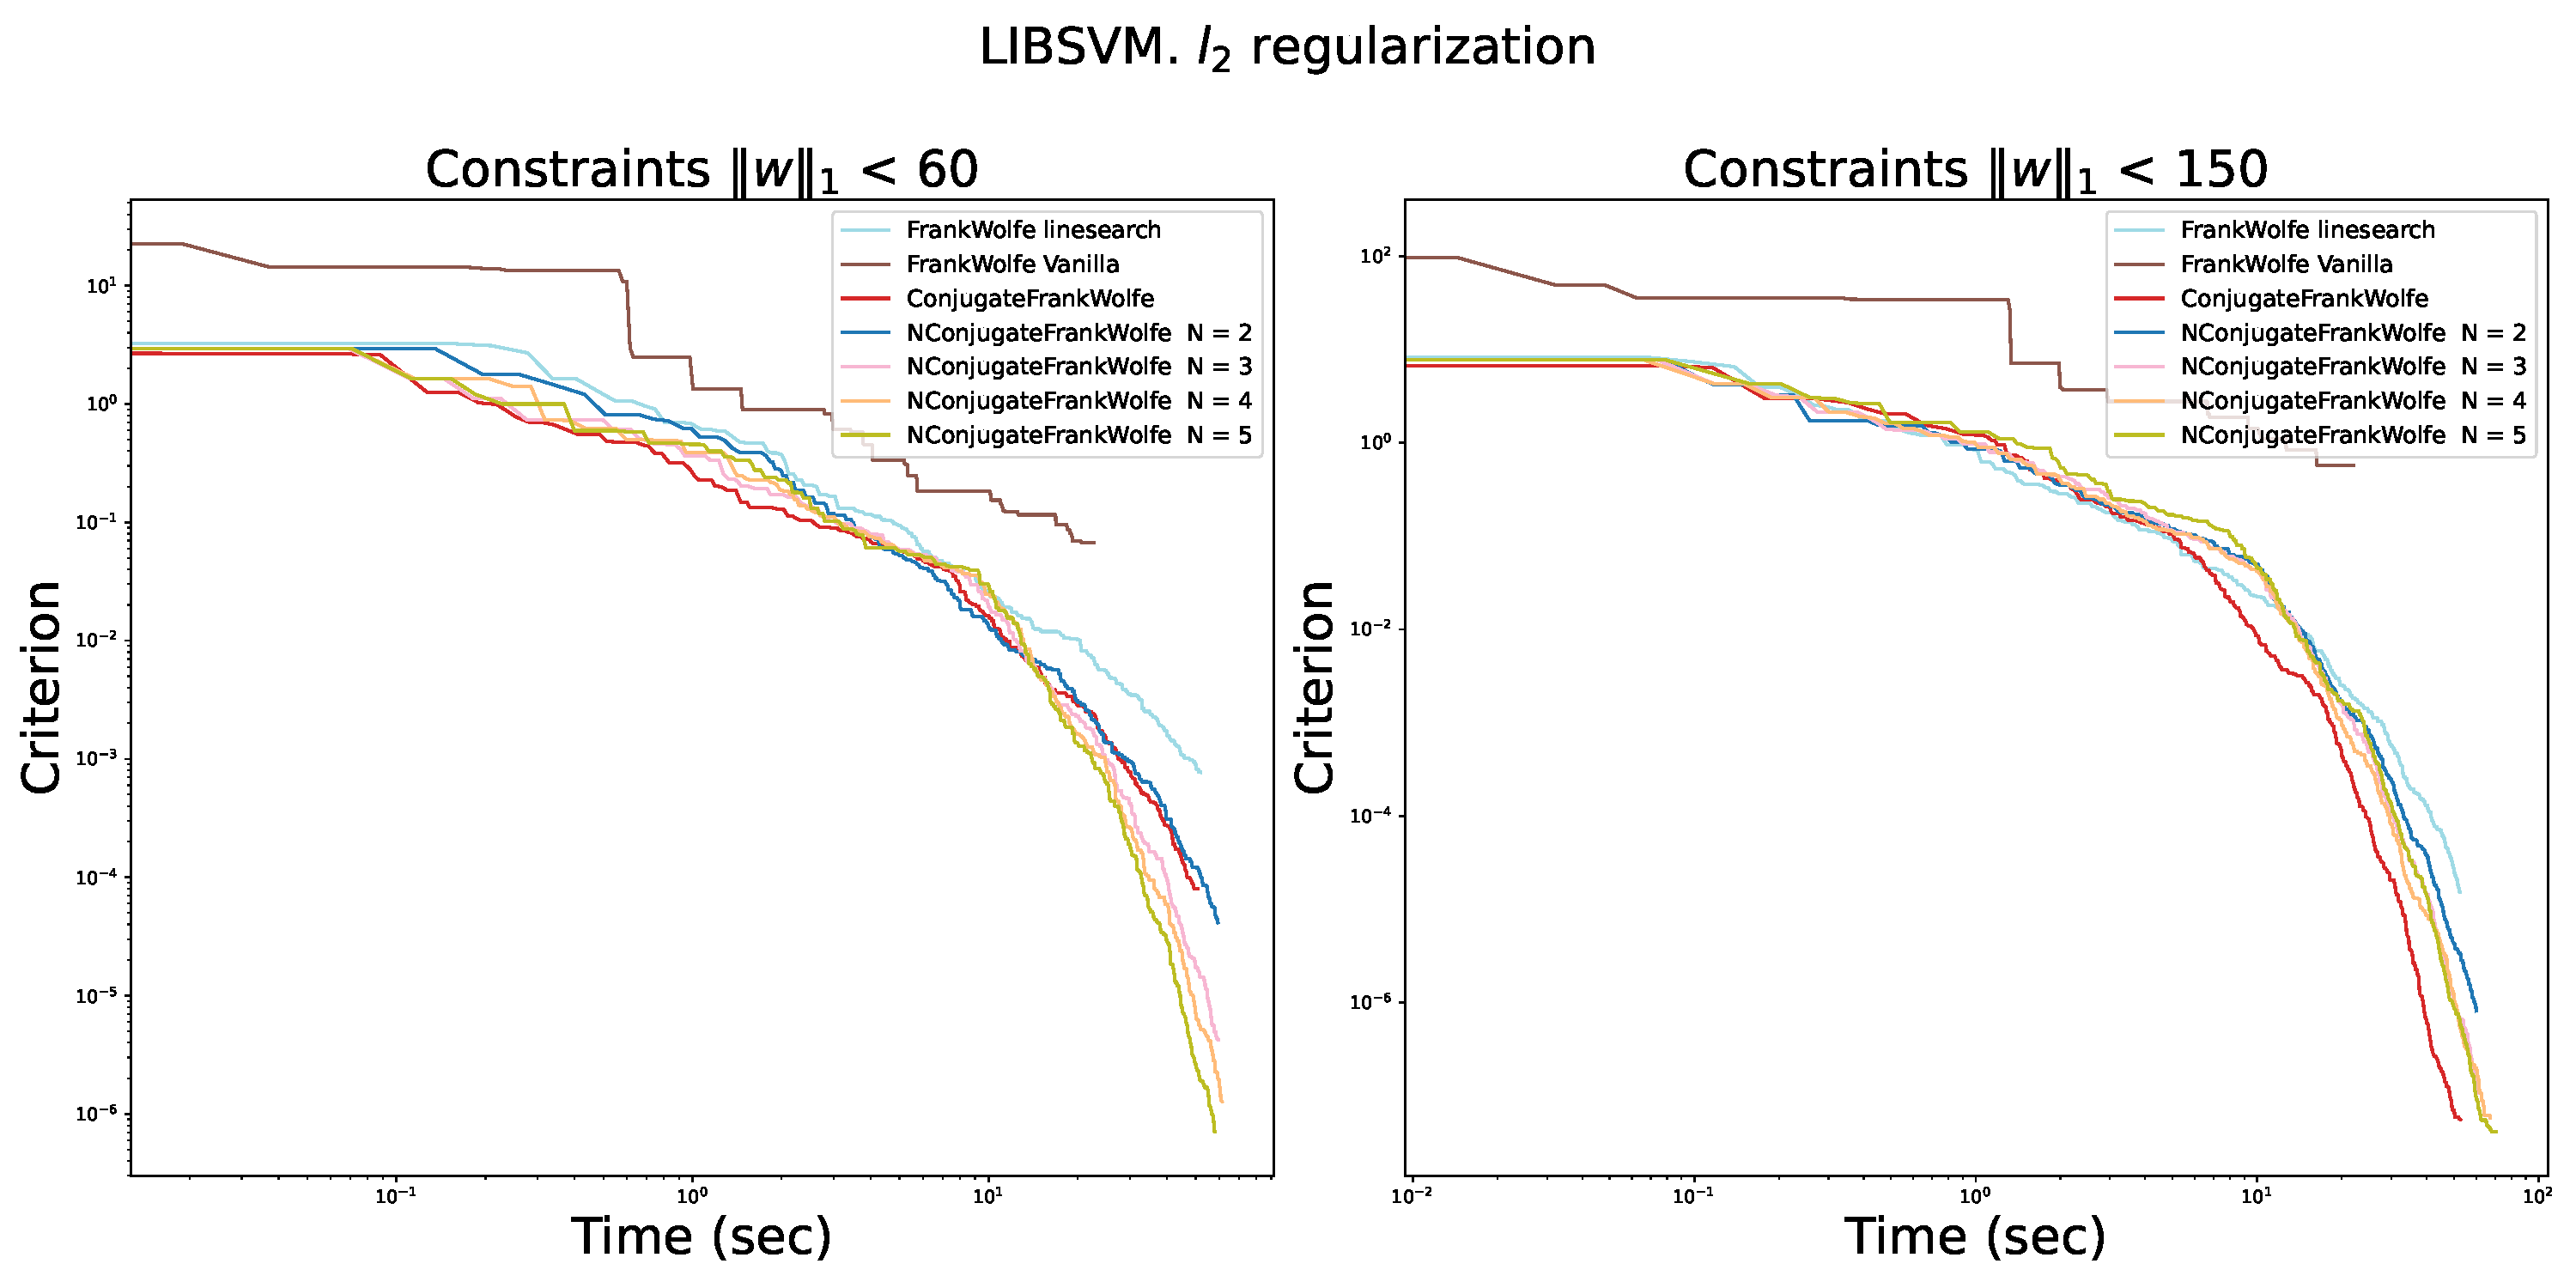
\includegraphics[width=0.96\textwidth]{cfw_ml/Experiment_6_fig_34.pdf}
\caption{Mushrooms с $l_2$-регуляризацией: сходимость FW, CFW и NFW по FW-зазору для больших значений радиуса $R$.}
\label{fig:cfw-ml-mushrooms-l2-34}
\end{figure}

\begin{figure}[H]
\centering
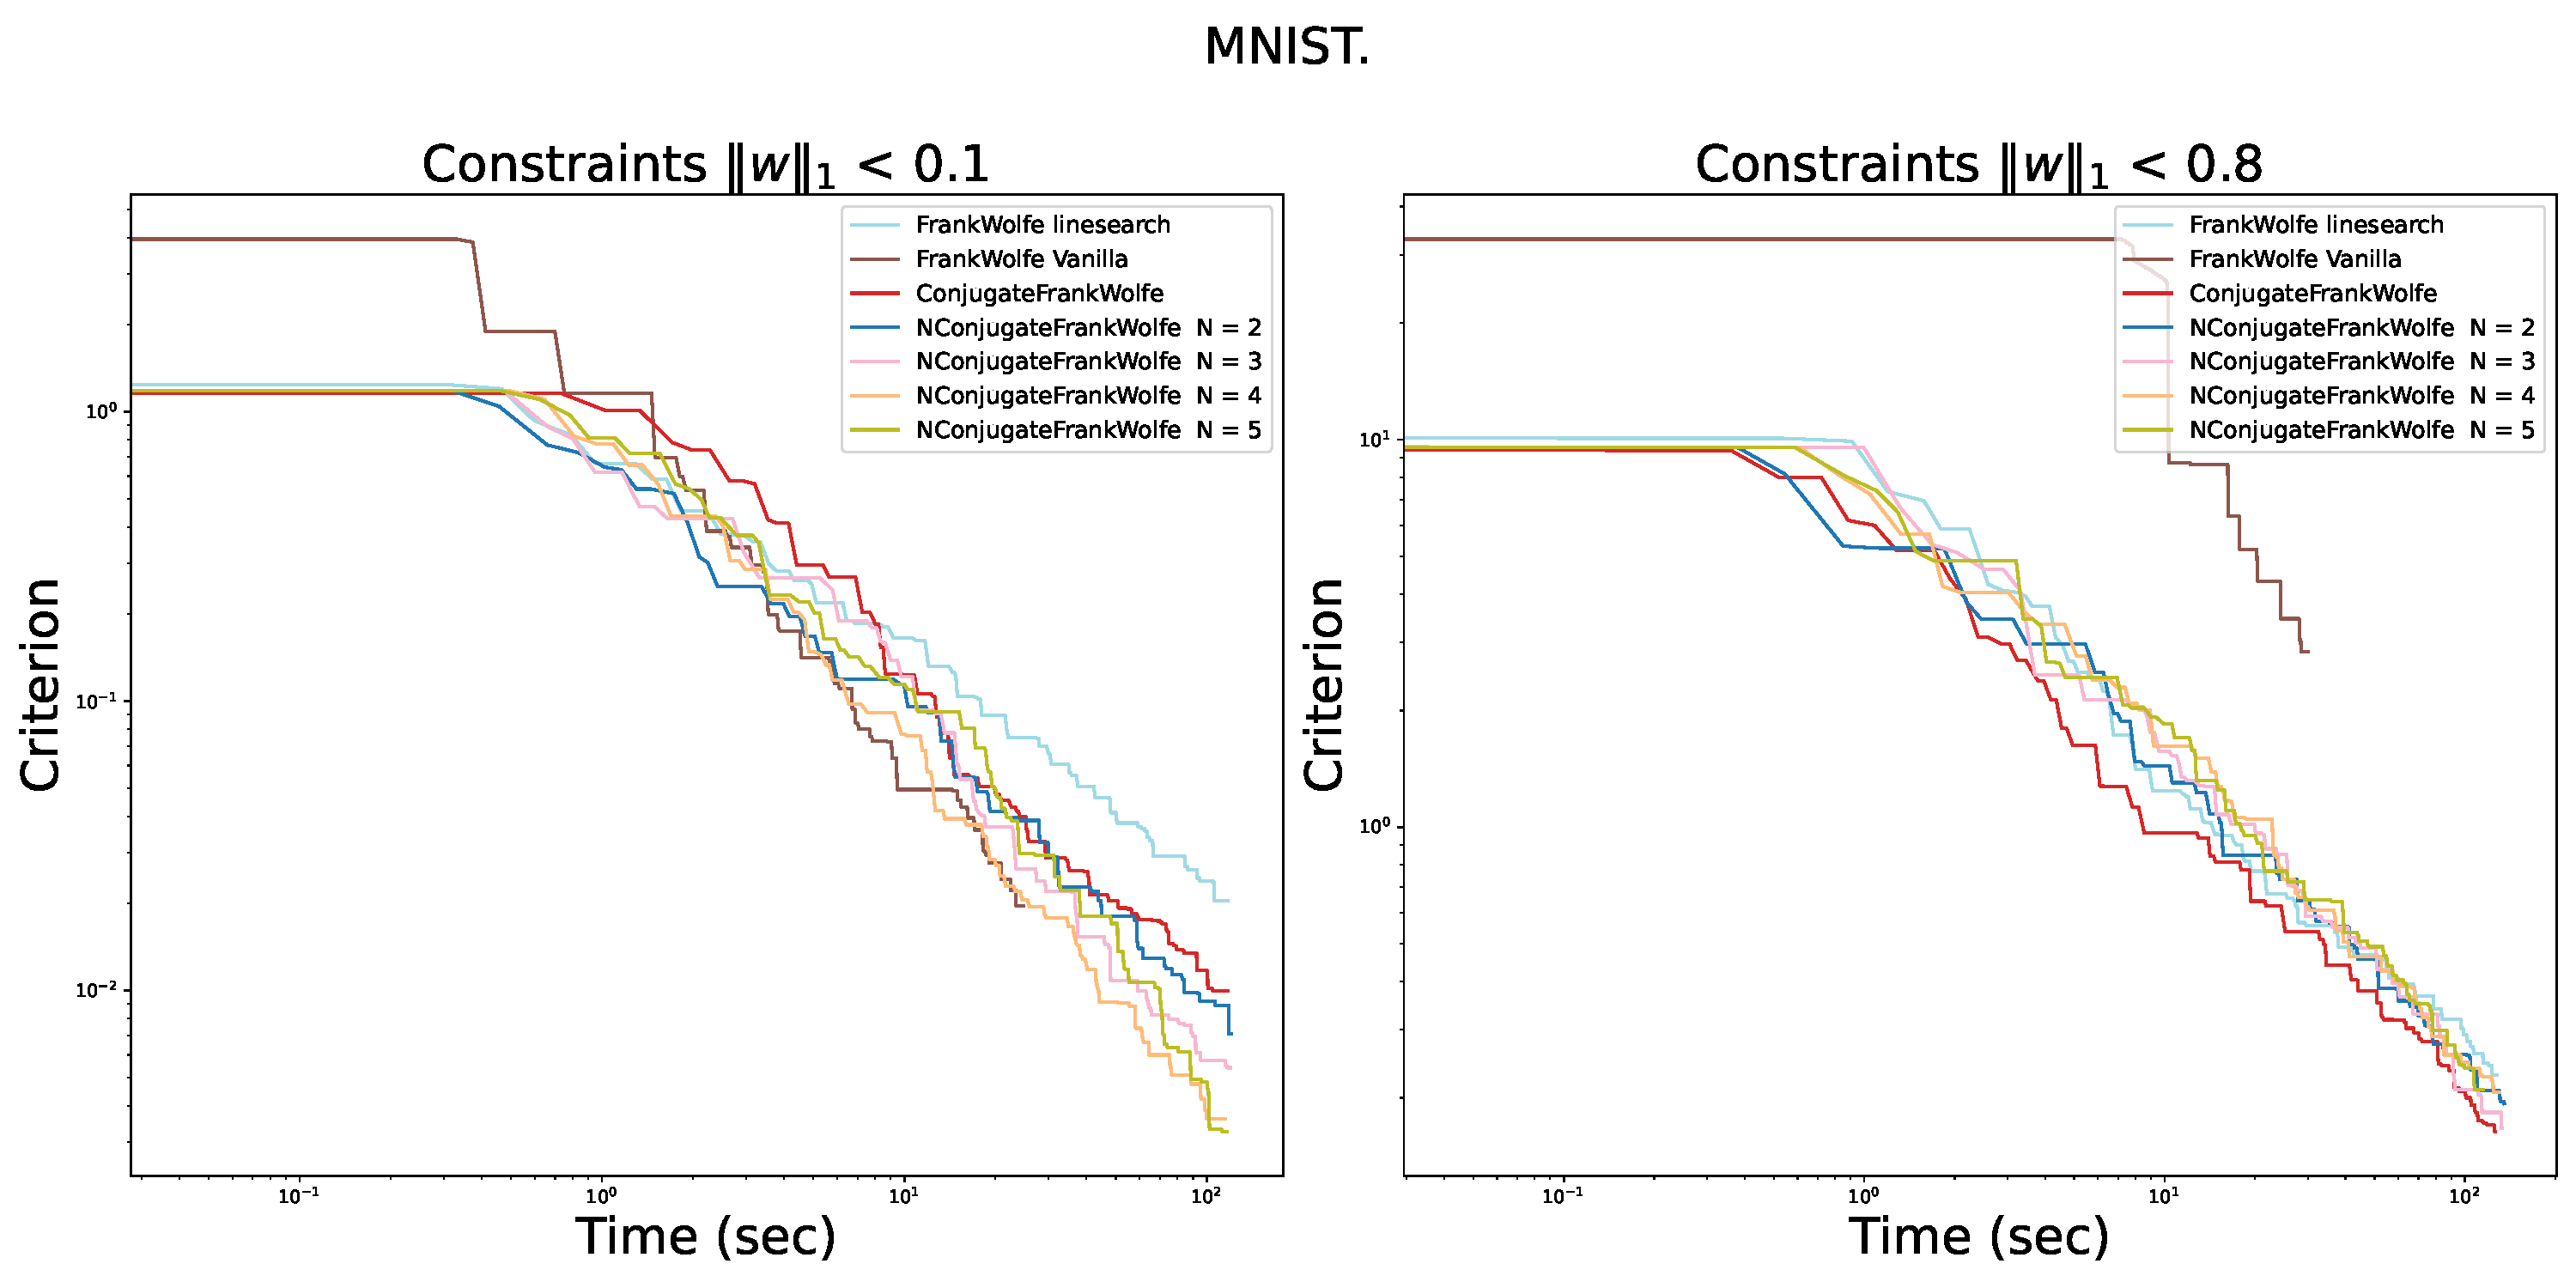
\includegraphics[width=0.96\textwidth]{cfw_ml/Experiment_7_fig_12.pdf}
\caption{MNIST без $l_2$-регуляризации: сходимость FW, CFW и NFW по FW-зазору для первых значений радиуса $R$.}
\label{fig:cfw-ml-mnist-12}
\end{figure}

\begin{figure}[H]
\centering
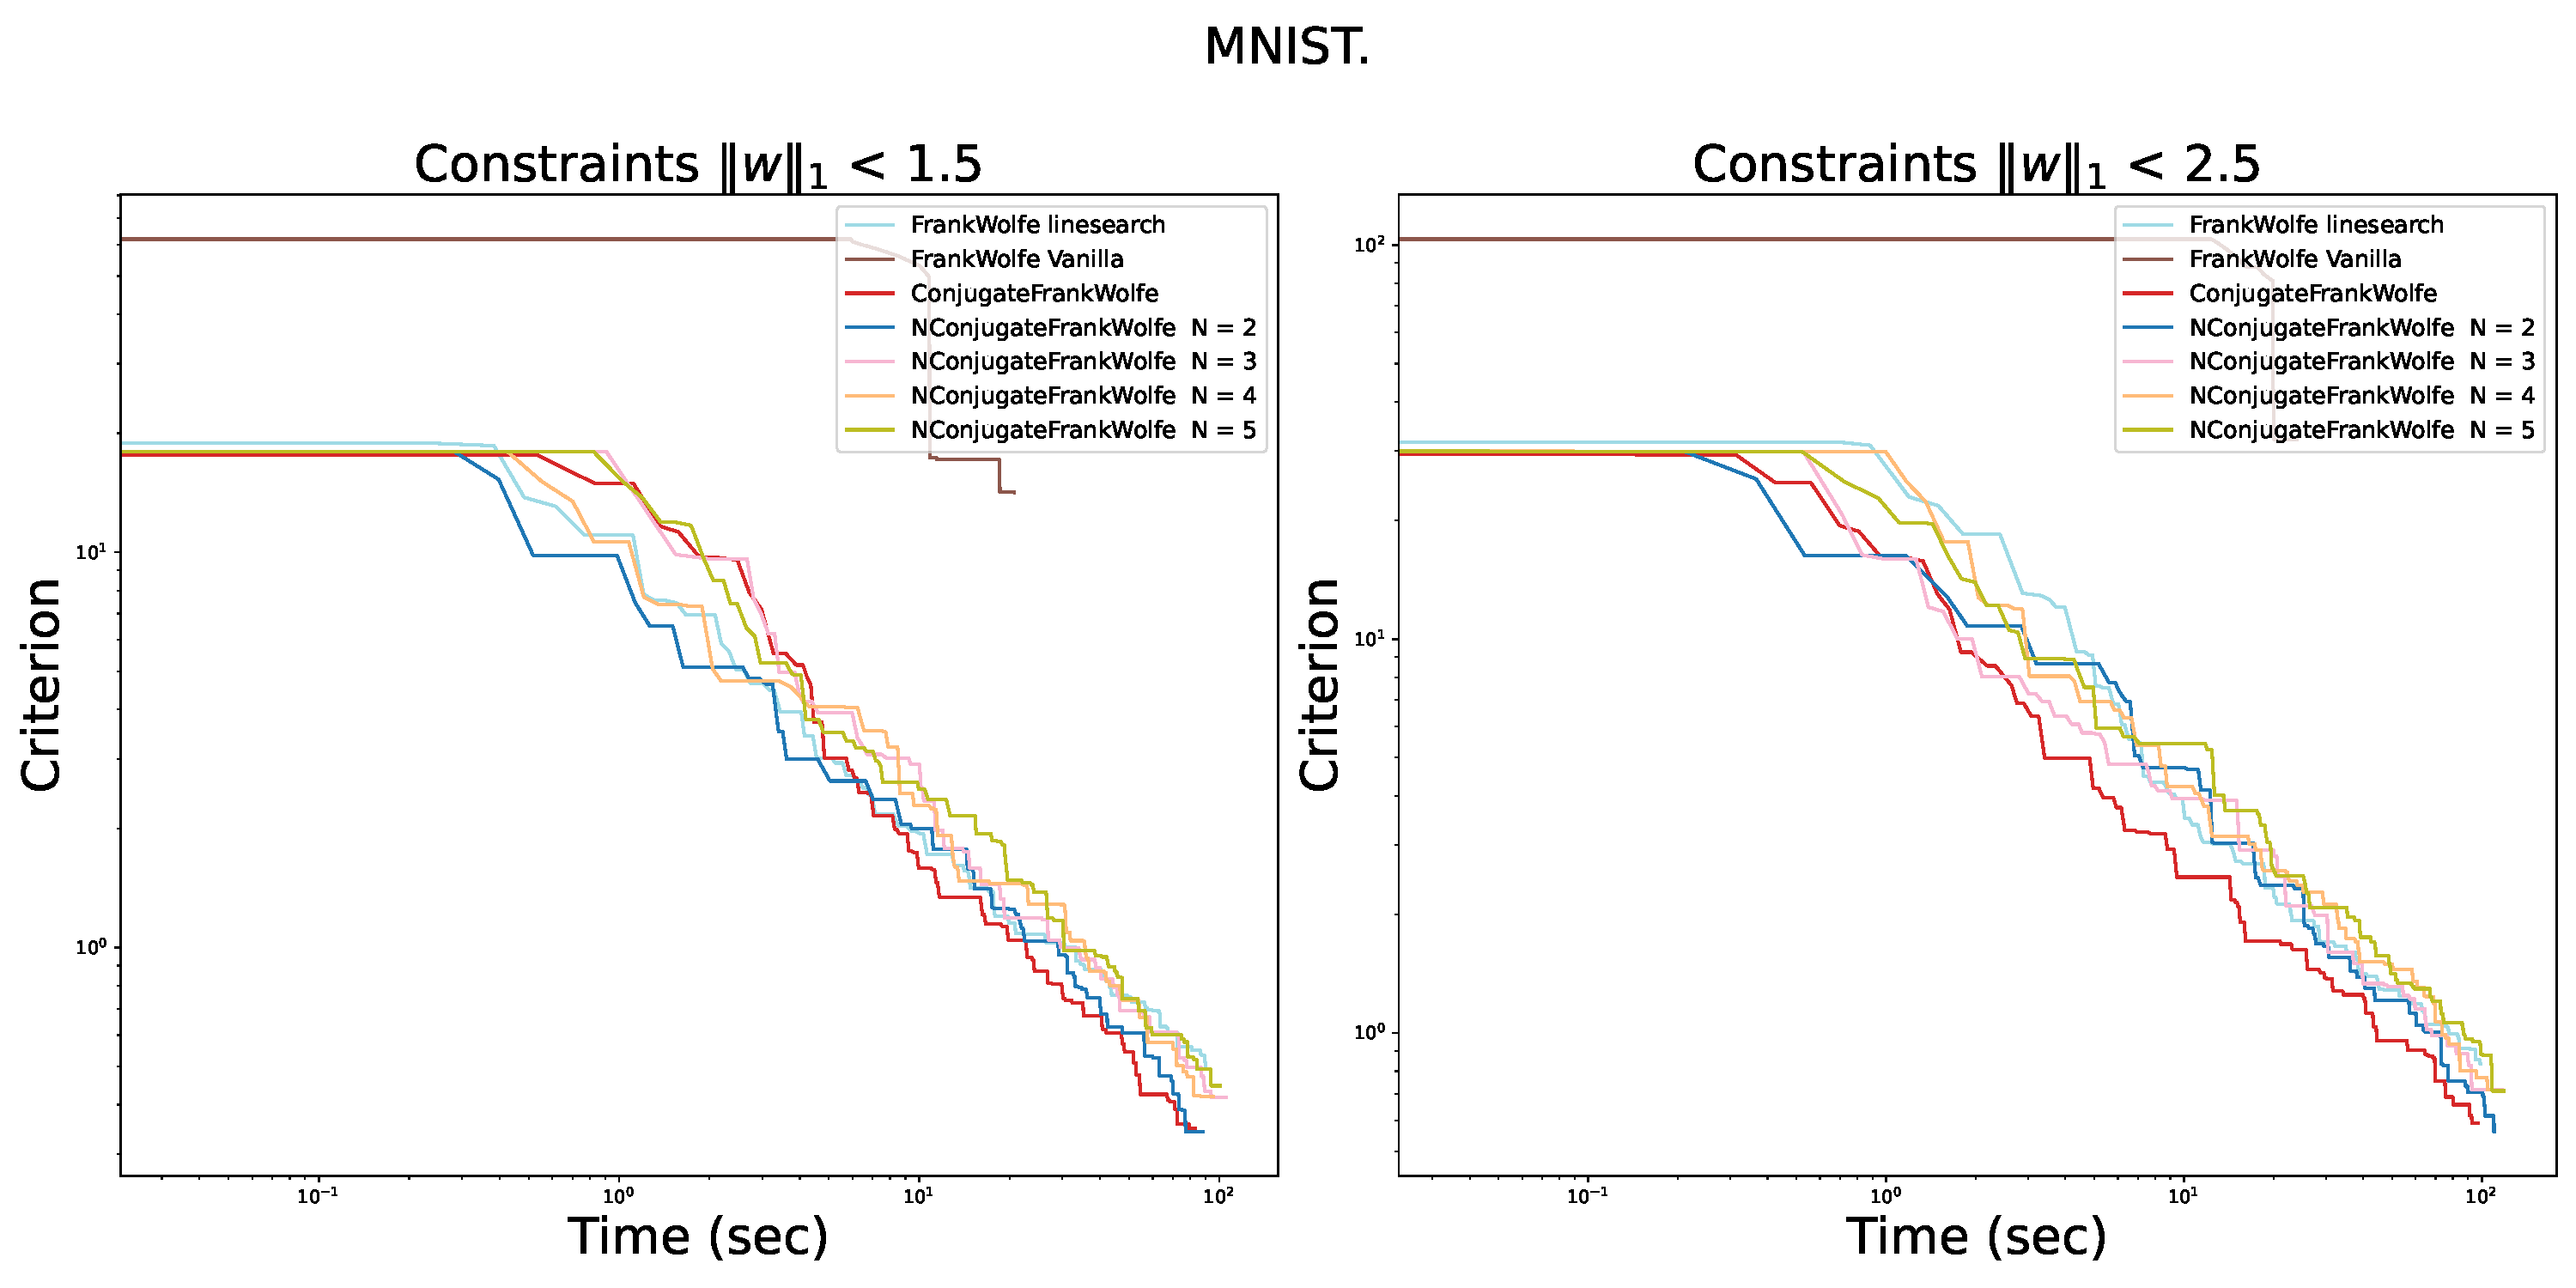
\includegraphics[width=0.96\textwidth]{cfw_ml/Experiment_7_fig_34.pdf}
\caption{MNIST без $l_2$-регуляризации: сходимость FW, CFW и NFW по FW-зазору для больших значений радиуса $R$.}
\label{fig:cfw-ml-mnist-34}
\end{figure}

\begin{figure}[H]
\centering
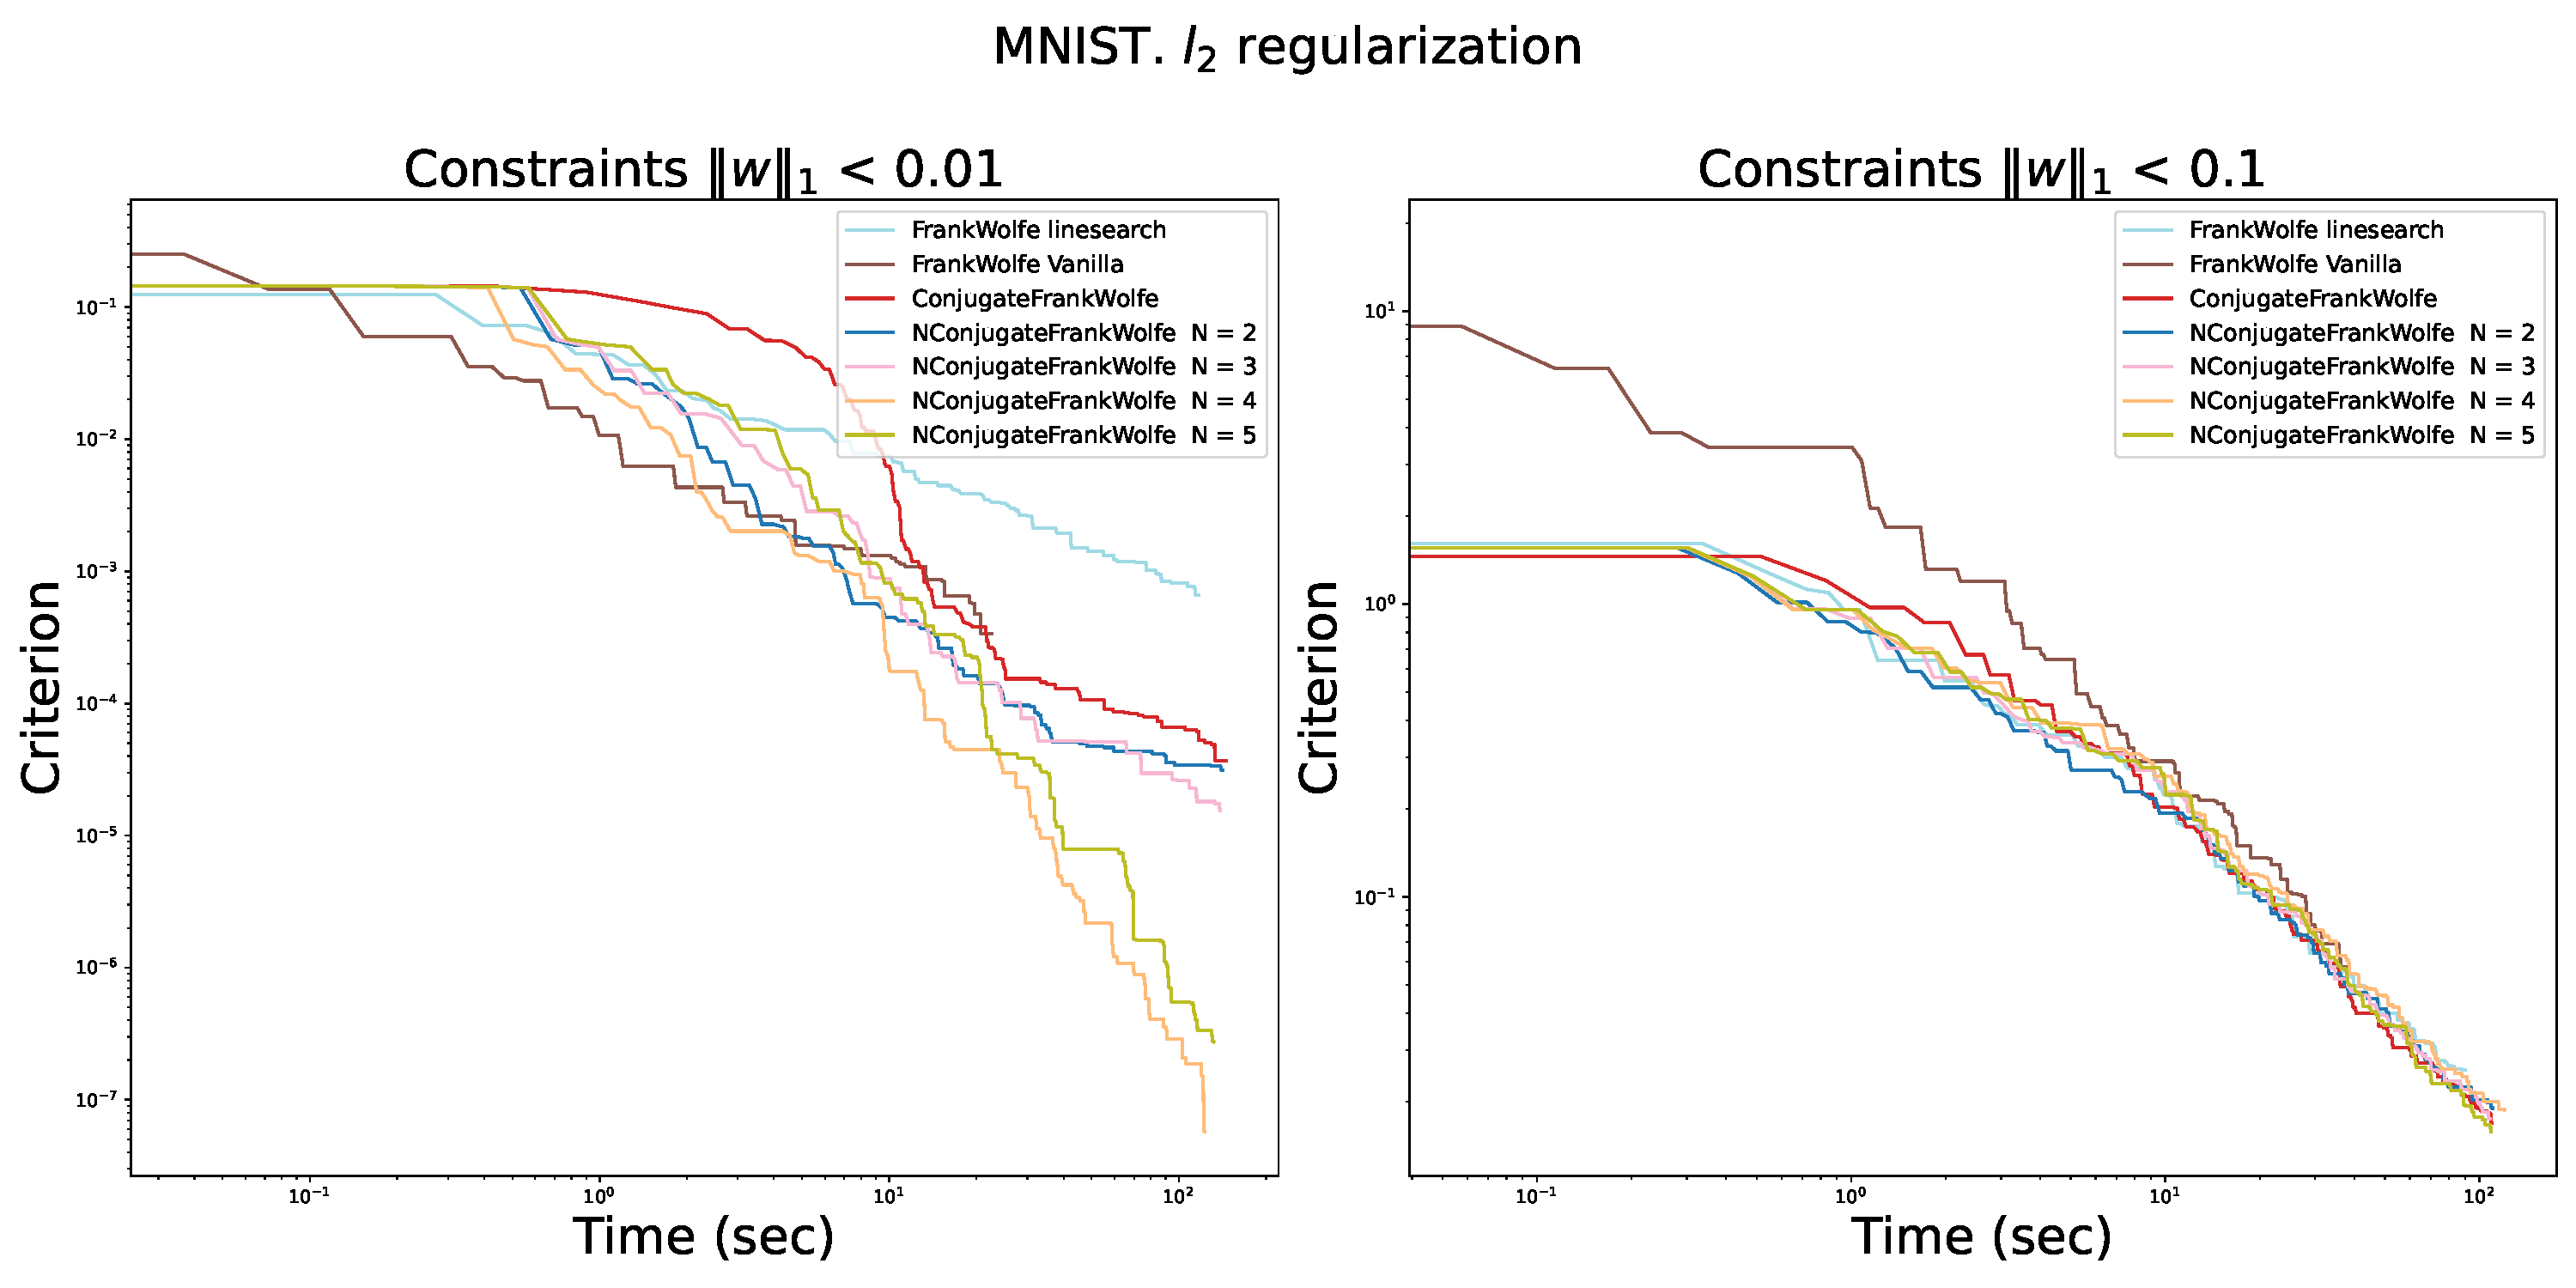
\includegraphics[width=0.96\textwidth]{cfw_ml/Experiment_8_fig_12.pdf}
\caption{MNIST с $l_2$-регуляризацией: сходимость FW, CFW и NFW по FW-зазору для первых значений радиуса $R$.}
\label{fig:cfw-ml-mnist-l2-12}
\end{figure}

\begin{figure}[H]
\centering
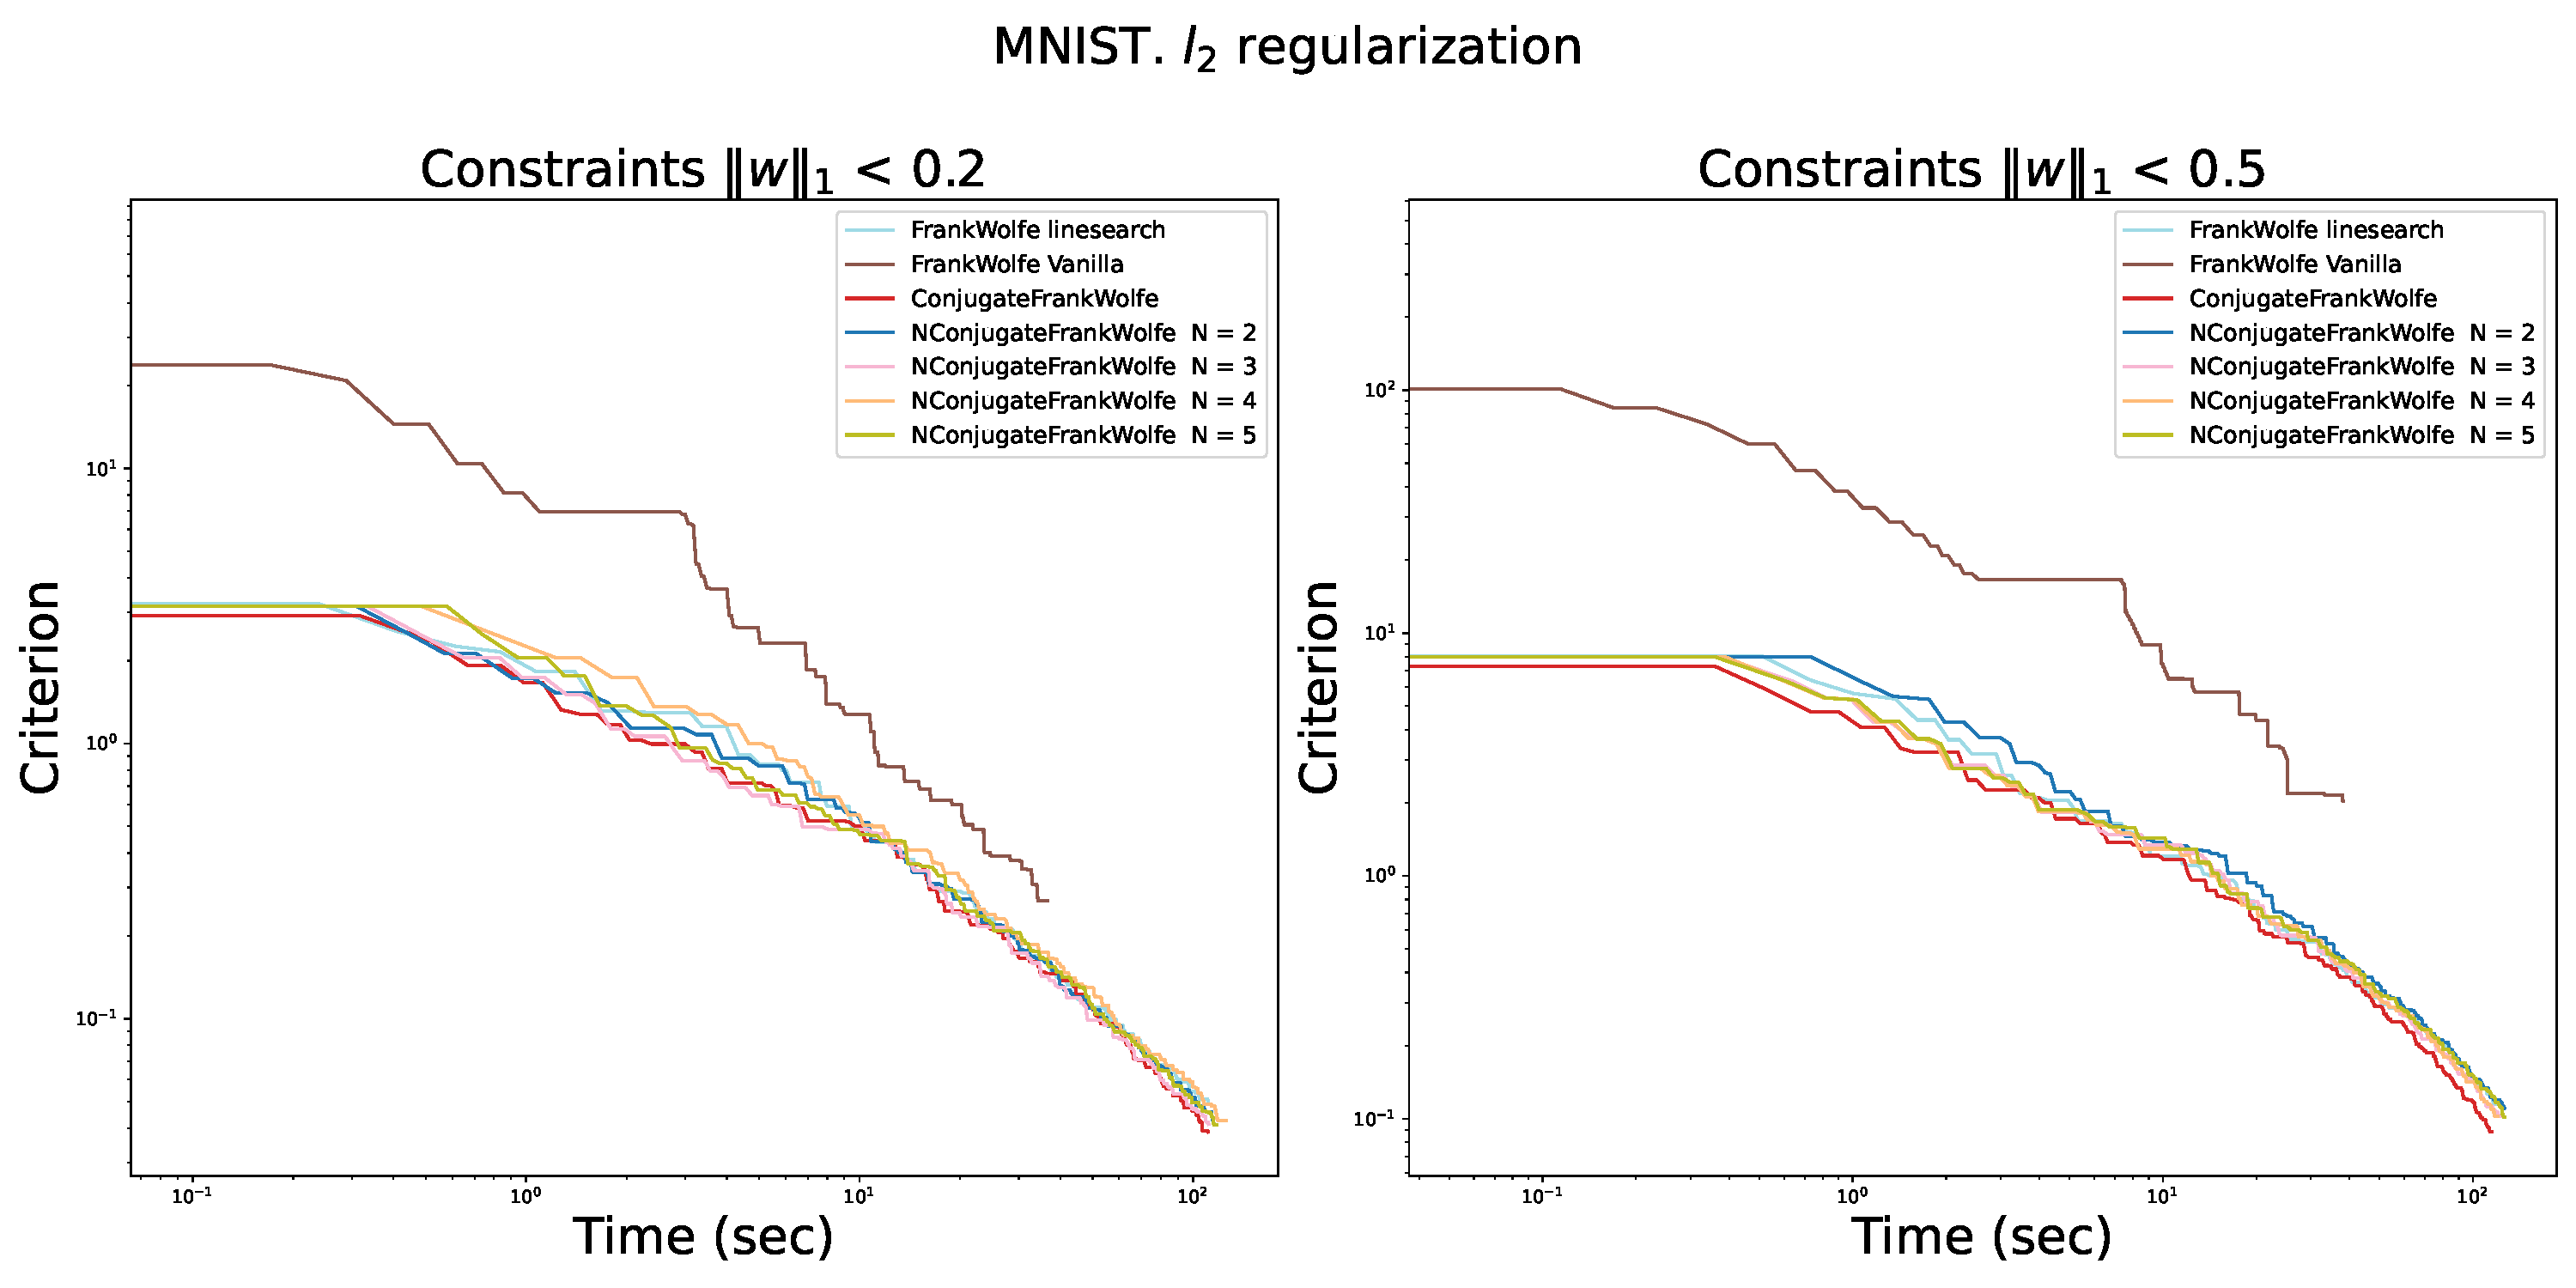
\includegraphics[width=0.96\textwidth]{cfw_ml/Experiment_8_fig_34.pdf}
\caption{MNIST с $l_2$-регуляризацией: сходимость FW, CFW и NFW по FW-зазору для больших значений радиуса $R$.}
\label{fig:cfw-ml-mnist-l2-34}
\end{figure}

Полученные результаты показывают:
\begin{enumerate}
    \item CFW и NFW часто существенно превосходят классический FW, особенно когда решение безусловной задачи далеко от границы допустимого множества.
    \item На Mushrooms преимущество сопряженных модификаций выражено сильнее, чем на MNIST.
    \item При близости безусловного решения к границе $\cX$ различия между FW с линейным поиском и CFW могут уменьшаться.
    \item Когда безусловное решение далеко от границы допустимого множества, NFW с числом предыдущих направлений больше двух часто сходится быстрее FW и CFW.
\end{enumerate}

\noindent\textbf{Экспериментальные таблицы.}

В таблицах ниже приведены численные результаты.
В каждой строке фиксируется радиус $R$ ограничения $\norm{w}_1\leq R$.
Значения в таблице являются достигнутым FW-зазором к моменту остановки по времени;
меньшее значение означает более качественное решение.
Лучший результат в строке выделен зеленым.

\begin{table}[H]
\centering
\caption{Mushrooms без $l_2$-регуляризации. Критерий -- FW-зазор.}
\label{tab:cfw-mushrooms-full}
\scriptsize
\resizebox{\textwidth}{!}{%
\begin{tabular}{lccccccc}
\toprule
$R$ & FW ls & FW & CFW & NFW $N=2$ & NFW $N=3$ & NFW $N=4$ & NFW $N=5$ \\
\midrule
5 & $9.93\cdot10^{-4}$ & $1.54\cdot10^{-4}$ & $4.46\cdot10^{-5}$ & \textcolor{green!50!black}{$9.72\cdot10^{-10}$} & $2.11\cdot10^{-9}$ & $2.49\cdot10^{-9}$ & $5.59\cdot10^{-9}$ \\
30 & $5.11\cdot10^{-3}$ & $2.05\cdot10^{-3}$ & $1.82\cdot10^{-3}$ & $3.19\cdot10^{-4}$ & $1.40\cdot10^{-4}$ & \textcolor{green!50!black}{$7.52\cdot10^{-5}$} & $2.72\cdot10^{-4}$ \\
60 & $3.82\cdot10^{-3}$ & $2.11\cdot10^{-3}$ & $1.12\cdot10^{-3}$ & $1.14\cdot10^{-3}$ & \textcolor{green!50!black}{$3.38\cdot10^{-4}$} & $6.59\cdot10^{-4}$ & $3.83\cdot10^{-4}$ \\
150 & $9.20\cdot10^{-4}$ & $3.06\cdot10^{-2}$ & $1.34\cdot10^{-4}$ & $4.06\cdot10^{-4}$ & $1.40\cdot10^{-4}$ & \textcolor{green!50!black}{$9.27\cdot10^{-5}$} & $1.47\cdot10^{-4}$ \\
\bottomrule
\end{tabular}}
\end{table}

\begin{table}[H]
\centering
\caption{Mushrooms с $l_2$-регуляризацией. Критерий -- FW-зазор.}
\label{tab:cfw-mushrooms-l2-full}
\scriptsize
\resizebox{\textwidth}{!}{%
\begin{tabular}{lccccccc}
\toprule
$R$ & FW ls & FW & CFW & NFW $N=2$ & NFW $N=3$ & NFW $N=4$ & NFW $N=5$ \\
\midrule
5 & $1.41\cdot10^{-3}$ & $3.71\cdot10^{-4}$ & $1.56\cdot10^{-5}$ & $4.42\cdot10^{-9}$ & \textcolor{green!50!black}{$3.30\cdot10^{-9}$} & $1.86\cdot10^{-8}$ & $4.86\cdot10^{-6}$ \\
30 & $8.96\cdot10^{-3}$ & $1.33\cdot10^{-2}$ & $6.21\cdot10^{-3}$ & $7.13\cdot10^{-3}$ & $5.61\cdot10^{-3}$ & $8.16\cdot10^{-3}$ & \textcolor{green!50!black}{$5.48\cdot10^{-3}$} \\
60 & $7.11\cdot10^{-3}$ & $6.69\cdot10^{-2}$ & $2.40\cdot10^{-3}$ & $2.12\cdot10^{-3}$ & $1.57\cdot10^{-3}$ & $1.13\cdot10^{-3}$ & \textcolor{green!50!black}{$9.26\cdot10^{-4}$} \\
150 & $1.82\cdot10^{-3}$ & $5.73\cdot10^{-1}$ & \textcolor{green!50!black}{$2.06\cdot10^{-4}$} & $1.22\cdot10^{-3}$ & $1.00\cdot10^{-3}$ & $5.40\cdot10^{-4}$ & $1.34\cdot10^{-3}$ \\
\bottomrule
\end{tabular}}
\end{table}

\begin{table}[H]
\centering
\caption{MNIST без $l_2$-регуляризации. Критерий -- FW-зазор.}
\label{tab:cfw-mnist-full}
\scriptsize
\resizebox{\textwidth}{!}{%
\begin{tabular}{lccccccc}
\toprule
$R$ & FW ls & FW & CFW & NFW $N=2$ & NFW $N=3$ & NFW $N=4$ & NFW $N=5$ \\
\midrule
$0.10$ & $7.48\cdot10^{-2}$ & \textcolor{green!50!black}{$1.97\cdot10^{-2}$} & $4.00\cdot10^{-2}$ & $3.87\cdot10^{-2}$ & $2.63\cdot10^{-2}$ & $2.06\cdot10^{-2}$ & $2.98\cdot10^{-2}$ \\
$0.80$ & $5.56\cdot10^{-1}$ & $2.83$ & \textcolor{green!50!black}{$5.37\cdot10^{-1}$} & $6.45\cdot10^{-1}$ & $5.88\cdot10^{-1}$ & $6.22\cdot10^{-1}$ & $6.48\cdot10^{-1}$ \\
$1.50$ & $1.15$ & $14.17$ & \textcolor{green!50!black}{$1.04$} & $1.25$ & $1.19$ & $1.45$ & $1.48$ \\
$2.50$ & $1.93$ & $32.05$ & \textcolor{green!50!black}{$1.63$} & $2.33$ & $2.11$ & $2.44$ & $2.51$ \\
\bottomrule
\end{tabular}}
\end{table}

\begin{table}[H]
\centering
\caption{MNIST с $l_2$-регуляризацией. Критерий -- FW-зазор.}
\label{tab:cfw-mnist-l2-full}
\scriptsize
\resizebox{\textwidth}{!}{%
\begin{tabular}{lccccccc}
\toprule
$R$ & FW ls & FW & CFW & NFW $N=2$ & NFW $N=3$ & NFW $N=4$ & NFW $N=5$ \\
\midrule
$0.01$ & $3.47\cdot10^{-3}$ & $3.38\cdot10^{-4}$ & $2.63\cdot10^{-4}$ & $1.41\cdot10^{-4}$ & $1.44\cdot10^{-4}$ & \textcolor{green!50!black}{$4.47\cdot10^{-5}$} & $5.62\cdot10^{-5}$ \\
$0.10$ & $5.39\cdot10^{-2}$ & $5.75\cdot10^{-2}$ & $4.93\cdot10^{-2}$ & \textcolor{green!50!black}{$4.69\cdot10^{-2}$} & $4.92\cdot10^{-2}$ & $6.02\cdot10^{-2}$ & $5.01\cdot10^{-2}$ \\
$0.20$ & $1.63\cdot10^{-1}$ & $2.68\cdot10^{-1}$ & $1.46\cdot10^{-1}$ & $1.60\cdot10^{-1}$ & \textcolor{green!50!black}{$1.42\cdot10^{-1}$} & $1.74\cdot10^{-1}$ & $1.65\cdot10^{-1}$ \\
$0.50$ & $4.10\cdot10^{-1}$ & $2.03$ & \textcolor{green!50!black}{$3.82\cdot10^{-1}$} & $4.65\cdot10^{-1}$ & $4.28\cdot10^{-1}$ & $4.35\cdot10^{-1}$ & $4.45\cdot10^{-1}$ \\
\bottomrule
\end{tabular}}
\end{table}

\noindent\textbf{Интерпретация ML-экспериментов.}

На Mushrooms без регуляризации безусловное решение имеет очень большую $l_1$-норму.
При радиусах $R=5,30,60,150$ оно находится далеко за пределами допустимого множества.
В этом режиме траектория FW часто упирается в границу $l_1$-шара и начинает менять активные
координаты зигзагообразно.
Именно здесь сопряженные методы дают наиболее заметный выигрыш.
Особенно сильный эффект виден при $R=5$, где NFW достигает зазора порядка $10^{-9}$,
а FW остается на уровнях $10^{-4}$--$10^{-3}$.

Для Mushrooms с $l_2$-регуляризацией безусловное решение имеет норму около $30.5$.
Поэтому при $R=30$ граница близка к естественному решению задачи, а при больших радиусах
часть ограничительного эффекта ослабевает.
Тем не менее CFW и NFW сохраняют преимущество над FW.
Интересно, что при $R=150$ лучшим оказывается CFW, а не NFW.
Это показывает, что увеличение памяти не является универсально лучшим выбором:
когда активная геометрия задачи становится менее жесткой, одного предыдущего направления
может быть достаточно.

На MNIST картина слабее.
Без регуляризации оценочная $l_1$-норма безусловного решения равна примерно $2.77$,
то есть часть выбранных радиусов находится близко к решению или внутри допустимой области.
В таких условиях FW с линейным поиском и CFW/NFW становятся близкими.
Однако даже здесь CFW часто дает лучший накопленный FW-зазор, особенно при $R=0.80,1.50,2.50$.
С $l_2$-регуляризацией безусловное решение имеет норму около $0.15$.
Поэтому при $R=0.01$ ограничение жесткое, и NFW с $N=4$ оказывается лучшим.
При $R=0.50$ ограничение уже сравнительно слабое, и лучшим становится CFW.

Общий вывод экспериментов таков:
\begin{enumerate}
    \item если безусловное решение далеко от границы $\cX$, сопряженные модификации резко ускоряют FW;
    \item если безусловное решение лежит близко к границе или внутри множества, разница между методами уменьшается;
    \item для простых и разреженных задач NFW с $N>2$ часто выигрывает у CFW;
    \item для более сложных задач с плотной структурой признаков эффект сопряженности проявляется слабее;
    \item зигзагообразность не исчезает полностью, но наступает позже, чем у классического FW.
\end{enumerate}

\subsection{Выводы по CFW in ML}

CFW и NFW можно применять не только в транспортном моделировании, но и в задачах машинного обучения, если они сводятся к гладкой выпуклой оптимизации на компактном выпуклом множестве.
Для таких задач явное вычисление гессиана не является обязательным: достаточно приближения произведения гессиана на вектор через разность градиентов.
Теоретически CFW сохраняет порядок сходимости FW по зазору Frank--Wolfe.
Практически же использование предыдущих направлений позволяет уменьшить зигзагообразность траектории и ускорить обучение логистической регрессии с ограничениями на параметры.

\newpage

\section{Стохастический блочно-координатный Frank--Wolfe}
\label{sec:scfw}

В этой главе рассматривается стохастический вариант Frank--Wolfe для крупномасштабной задачи равновесного распределения потоков~\cite{ignashin2026stochastic}.
Этот вариант удобно называть Stochastic Origin Frank--Wolfe (SOFW).
В контексте данной работы он рассматривается как специальный случай блочно-координатного FW (BCFW) со стохастическим выбором блоков.
Его ключевая идея состоит в выборе случайных блоков и обновлении только части координат на каждой итерации.

Классический FW в транспортной задаче требует на каждой итерации найти кратчайшие пути от всех источников ко всем стокам.
Если граф содержит много зон и узлов, стоимость одной итерации становится основной вычислительной проблемой.
Стохастический подход уменьшает стоимость итерации: вместо полного линейного оракула выбирается случайное подмножество источников или OD-пар, а остальные блоки фиксируются.

\subsection{Блочная структура транспортной задачи}

Рассмотрим вектор потоков по путям как конкатенацию блоков по OD-парам:
\[
    x=
    \left(x^{(i,j)}\right)_{(i,j)\in OD},
    \qquad
    x^{(i,j)}\in\R^{|\cP_{i,j}|}.
\]
Каждый блок соответствует множеству путей $\cP_{i,j}$ между источником $i$ и стоком $j$.
Для блока выполняются ограничения спроса
\[
    \sum_{p\in\cP_{i,j}}x_p=d_{ij},
    \qquad
    x_p\geq 0.
\]
Следовательно, допустимое множество потоков по путям является декартовым произведением:
\[
    \cX=
    \prod_{(i,j)\in OD}\cX^{(i,j)}.
\]
Переход от потоков по путям к потокам по ребрам задается линейным отображением
\[
    F(x)=\Theta x,
    \qquad
    f=F(x).
\]

В классическом FW линейный оракул решается по всем блокам:
\[
    s_k\in
    \argmin_{x\in\cX}
    \inner{\nabla\Psi(F(x_k))}{F(x)}.
\]
Так как
\[
    \inner{\nabla\Psi(F(x_k))}{F(x)}
    =
    \sum_{(i,j)\in OD}
    \inner{\tau(f_k)}{\Theta_{ij}x^{(i,j)}},
\]
оракул распадается на независимые подзадачи по OD-парам.
Каждая такая подзадача является назначением всего спроса на кратчайший путь при текущих дорожных временах.

\subsection{Stochastic Origin Frank--Wolfe}

На итерации $k$ SOFW выбирает случайное подмножество OD-пар $\cI_k\subset OD$ и обновляет только соответствующие блоки.
Остальные блоки фиксируются в текущих значениях:
\[
    \cX_k
    =
    \left\{
        x\in\cX
        \;\middle|\;
        x^{(i,j)}=x_k^{(i,j)}
        \text{ для всех }(i,j)\notin\cI_k
    \right\}.
\]
Линейный оракул решается на суженном множестве:
\[
    s_k
    \in
    \argmin_{x\in\cX_k}
    \inner{\nabla\Psi(f_k)}{F(x)}.
\]
На практике удобно выбирать не отдельные OD-пары, а подмножество источников.
Если выбран источник $i$, то в батч включаются все корреспонденции $(i,j)$.
Это позволяет один раз запустить алгоритм Дейкстры от источника $i$ и получить кратчайшие пути до всех стоков.

\subsection{Статическое назначение потоков и роль модели Бекмана}

SOFW мотивируется задачей прогнозирования транспортных потоков.
В транспортном планировании требуется оценить распределение движения по дорожной сети
при заданной матрице спроса.
В статической модели считается, что спрос за рассматриваемый период фиксирован,
а равновесие описывается принципом Вардропа: все используемые пути между одной OD-парой
имеют минимальное время движения, а неиспользуемые пути не короче используемых.

Модель Бекмана дает выпуклую оптимизационную формулировку этого равновесия:
\[
    \min_{f=\Theta x,\;x\in\cX}
    \Psi(f)=
    \sum_{e\in\cE}\int_0^{f_e}\tau_e(z)\,dz.
\]
Если функции $\tau_e$ неубывающие, то задача выпукла.
Оптимальность $x^\ast$ означает, что для любой допустимой перераспределенной траектории
$x$ выполнено вариационное неравенство
\[
    \inner{\tau(f^\ast)}{\Theta x-\Theta x^\ast}\geq 0.
\]
Это ровно условие равновесия: нельзя уменьшить суммарную линейную стоимость при текущих
временах движения.

Классический FW применим здесь особенно естественно.
Линейная подзадача
\[
    \min_{x\in\cX}\inner{\tau(f^k)}{\Theta x}
\]
распадается по OD-парам:
\[
    \min_{x^{(i,j)}\in\cX^{(i,j)}}
    \sum_{p\in\cP_{i,j}}x_p
    \sum_{e\in p}\tau_e(f^k_e).
\]
Оптимум достигается назначением всего спроса $d_{ij}$ на кратчайший путь.
Поэтому каждая полная итерация FW фактически состоит из набора запусков алгоритма
кратчайших путей.

\subsection{Path-based и link-based представления}

В теории удобно работать с путевыми потоками $x$, потому что допустимое множество имеет
явную блочную структуру:
\[
    \cX=\prod_{(i,j)\in OD}
    \left\{
        x^{(i,j)}\geq 0\;\middle|\;
        \sum_{p\in\cP_{i,j}}x_p=d_{ij}
    \right\}.
\]
Однако число возможных путей может быть экспоненциальным.
Поэтому в реализации обычно не хранится весь вектор $x$.
Хранятся потоки по ребрам $f$, а очередное решение линейного оракула строится как
all-or-nothing assignment: для каждой OD-пары весь спрос временно отправляется на текущий
кратчайший путь.

SOFW требует больше информации, чем полный FW.
Если обновляется только часть источников, нужно уметь вычесть старый вклад этих источников
из суммарного потока и добавить новый.
Поэтому алгоритм хранит разложение
\[
    f=\sum_{o\in O}f^{(o)},
\]
где $f^{(o)}$ -- поток по ребрам, порожденный спросом из источника $o$.
Когда выбран батч источников $\mathcal A_k$, обновляются только компоненты
$f^{(o)}$, $o\in\mathcal A_k$, а остальные остаются фиксированными.
Именно это разложение объясняет главный компромисс метода: SOFW уменьшает время итерации,
но требует больше памяти.

\begin{algorithm}
\caption{Stochastic Origin Frank--Wolfe}
\label{alg:sofw}
\begin{algorithmic}
\REQUIRE допустимое множество $\cX=\prod_{w\in OD}\cX^w$, отображение $F(x)=\Theta x$, вероятности выбора блоков, шаги $\gamma_k$
\STATE выбрать начальное $x_0\in\cX$ и положить $f_0=F(x_0)$
\FOR{$k=0,1,2,\ldots$}
\STATE выбрать случайное подмножество $\cI_k\subset OD$
\STATE определить суженное множество
\[
    \cX_k=
    \left(\prod_{w\in\cI_k}\cX^w\right)
    \times
    \left(\prod_{w\notin\cI_k}\{x_k^w\}\right)
\]
\STATE вычислить $s_k\in\argmin_{x\in\cX_k}\inner{\nabla\Psi(f_k)}{F(x)}$
\STATE вычислить направление $d_k=F(s_k)-F(x_k)$ или его взвешенную несмещенную оценку
\STATE обновить $f_{k+1}=f_k+\gamma_kd_k$
\STATE обновить $x_{k+1}=x_k+\gamma_k(s_k-x_k)$
\ENDFOR
\end{algorithmic}
\end{algorithm}

\subsection{Взвешенный вариант}

Во взвешенном варианте источники выбираются с вероятностями, пропорциональными суммарному спросу.
Пусть
\[
    d_i=\sum_j d_{ij},
    \qquad
    \cC_i=\{(i,j)\in OD\}.
\]
Здесь $d_i$ -- полный спрос, исходящий из источника $i$, а $\cC_i$ -- множество всех
корреспонденций с этим источником.
В качестве веса источника можно взять нормированный спрос
\[
    w_i
    =
    \frac{d_i}{\sum_{\ell}d_\ell},
    \qquad
    \sum_i w_i=1.
\]
Тогда источник $i$ выбирается с вероятностью $w_i$.
Если после выбора источника корреспонденция внутри $\cC_i$ выбирается равномерно, то
вес OD-блока $(i,j)$ равен
\[
    w_{ij}
    =
    \mathbb{P}\{(i,j)\}
    =
    w_i
    \cdot
    \frac{1}{|\cC_i|}
    =
    \frac{d_i}{\sum_{\ell}d_\ell}
    \cdot
    \frac{1}{|\cC_i|}.
\]
Такой выбор чаще обновляет источники с большим суммарным спросом.
На практике можно выбирать сразу батч источников с вероятностями $w_i$ и затем включать
в батч все корреспонденции выбранных источников; это соответствует той же идее, но лучше
согласуется с вычислением кратчайших путей от одного источника ко всем стокам.

Для сохранения несмещенности направления используется importance-weighted коррекция:
\[
    d_k
    =
    \frac{1}{|\cI_k|}
    W_k
    \sum_{(i,j)\in\cI_k}
    \frac{1}{w_{ij}}
    \left(
        F(s_k^{[(i,j)]})-F(x_k^{[(i,j)]})
    \right),
    \qquad
    W_k=
    \left(
        \sum_{(i,j)\in\cI_k}\frac{1}{w_{ij}}
    \right)^{-1}.
\]

\subsection{Сходимость}

Сходимость SOFW следует из анализа Block-Coordinate Frank--Wolfe на произведениях множеств~\cite{lacoste2013block,jaggi2012blockcoordfw}.
Для каждого блока $w=(i,j)$ вводится блочная константа кривизны:
\[
C_\Psi^w
=
\sup
\frac{2}{\gamma^2}
\left[
    \Psi(F(y))
    -
    \Psi(F(x))
    -
    \inner{\nabla\Psi(F(x))}{F(y^{[w]})-F(x^{[w]})}
\right],
\]
где супремум берется по $x\in\cX$, $s^w\in\cX^w$, $\gamma\in[0,1]$ и
\[
    y=x+\gamma(s^{[w]}-x^{[w]}).
\]
Суммарная блочная кривизна равна
\[
    C_\Psi^\otimes=\sum_{w\in OD}C_\Psi^w.
\]

Если на каждой итерации выбирается одна OD-пара равномерно случайно, то для ожидаемой субоптимальности выполняется оценка
\begin{equation}
    \E[\Psi(f_k)]-\Psi(f^\ast)
    \leq
    \frac{2|OD|}{k+2|OD|}
    \left[
        C_\Psi^\otimes+\Psi(f_0)-\Psi(f^\ast)
    \right].
    \label{eq:sofw-rate-single}
\end{equation}
Для батчевого варианта, где на итерации выбирается подмножество $\cI_k$ размера $m$, направление можно записать как
\[
    d_k=
    \frac{1}{m}
    \sum_{w\in\cI_k}
    \left(s_k^{[w]}-x_k^{[w]}\right),
    \qquad
    x_{k+1}=x_k+\gamma_kd_k.
\]
При равномерном выборе без возвращения условное математическое ожидание прогресса имеет тот же вид, что и в небатчевом случае:
\[
    \E[\Psi(F(x_{k+1}))\mid x_k]
    \leq
    \Psi(F(x_k))
    -
    \frac{\gamma_k}{|OD|}g(x_k)
    +
    \frac{\gamma_k^2}{2|OD|}C_\Psi^\otimes.
\]

\begin{theorem}
\label{thm:sofw-batched-rate}
Пусть $\{x_k\}$ порождается батчевым SOFW с произвольным размером батча $m$ и шагами
\[
    \gamma_k=\frac{2|OD|}{k+2|OD|}.
\]
Тогда
\[
    \E[\Psi(F(x_k))]-\Psi(F(x^\ast))
    \leq
    \frac{2|OD|}{k+2|OD|}
    \left[
        C_\Psi^\otimes+\Psi(F(x_0))-\Psi(F(x^\ast))
    \right].
\]
Следовательно, для достижения $\varepsilon$-точности в ожидании достаточно
\[
    \mathcal{O}\left(\frac{|OD|}{\varepsilon}\right)
\]
итераций.
\end{theorem}

Батчирование в такой нормировке не улучшает теоретический порядок по числу итераций, но уменьшает дисперсию направления и может существенно улучшать время работы.
В транспортной задаче это особенно важно, поскольку стоимость итерации почти линейно зависит от числа источников, для которых запускается поиск кратчайших путей.

\subsection{Доказательство батчевой оценки}

Доказательство для батчевого SOFW начинается с явного разложения полного FW-зазора по
OD-блокам.
Пусть выбран блок $w\in OD$ и
\[
    s^w(x)\in
    \argmin_{u\in\cX^w}
    \inner{\nabla\Psi(F(x))}{F(u^{[w]})}.
\]
Здесь $u^{[w]}$ означает вектор, у которого активен только блок $w$.
Определим блочный FW-зазор
\[
    g^w(x)
    =
    \inner{\nabla\Psi(F(x))}
    {F\left((x^w-s^w(x))^{[w]}\right)}
    \geq 0.
\]
Тогда полный FW-зазор раскладывается в сумму
\[
    g(x)
    =
    \sum_{w\in OD}g^w(x).
\]
Это равенство является ключевым: линейный оракул в модели Бекмана распадается по
OD-парам, поэтому потеря от обновления только части блоков выражается через долю
неиспользованных слагаемых в этой сумме.

Обновление только этого блока имеет вид
\[
    x^+=x+\gamma(s^w(x)-x^w)^{[w]}.
\]
По определению блочной кривизны
\[
    \Psi(F(x^+))
    \leq
    \Psi(F(x))
    -
    \gamma g^w(x)
    +
    \frac{\gamma^2}{2}C_\Psi^w.
\]
Если блок выбирается равномерно, то после взятия условного ожидания получается
\[
    \E[g^w(x)\mid x]
    =
    \frac{1}{|OD|}\sum_{w\in OD}g^w(x)
    =
    \frac{1}{|OD|}g(x).
\]
Аналогично
\[
    \E[C_\Psi^w]=\frac{1}{|OD|}C_\Psi^\otimes.
\]
Отсюда следует рекурсия
\[
    \E[\Psi(F(x_{k+1}))\mid x_k]
    \leq
    \Psi(F(x_k))
    -
    \frac{\gamma_k}{|OD|}g(x_k)
    +
    \frac{\gamma_k^2}{2|OD|}C_\Psi^\otimes.
\]

Для батча размера $m$ направление записывается как среднее по выбранным блокам:
\[
    d_k
    =
    \frac{1}{m}
    \sum_{w\in\cI_k}
    (s^w(x_k)-x_k^w)^{[w]}.
\]
Поскольку $F$ линейно, а $\Psi$ выпукла, точку после батчевого шага можно сравнить со
средним одноблочных шагов:
\[
    x_k+\gamma d_k
    =
    \frac{1}{m}
    \sum_{w\in\cI_k}
    \left(
        x_k+\gamma(s^w(x_k)-x_k^w)^{[w]}
    \right).
\]
Следовательно,
\[
    \Psi(F(x_k+\gamma d_k))
    \leq
    \frac{1}{m}
    \sum_{w\in\cI_k}
    \Psi\left(
        F\left(x_k+\gamma(s^w(x_k)-x_k^w)^{[w]}\right)
    \right).
\]
Подставляя одноблочную оценку в правую часть, получаем
\[
    \Psi(F(x_k+\gamma d_k))
    \leq
    \Psi(F(x_k))
    -
    \frac{\gamma}{m}
    \sum_{w\in\cI_k}g^w(x_k)
    +
    \frac{\gamma^2}{2m}
    \sum_{w\in\cI_k}C_\Psi^w.
\]
Если блоки выбираются равномерно без возвращения, то каждый блок попадает в батч с
вероятностью $m/|OD|$.
Поэтому
\[
    \E\left[
        \frac{1}{m}\sum_{w\in\cI_k}g^w(x_k)
        \;\middle|\;x_k
    \right]
    =
    \frac{1}{|OD|}\sum_{w\in OD}g^w(x_k)
    =
    \frac{1}{|OD|}g(x_k),
\]
и аналогично
\[
    \E\left[
        \frac{1}{m}\sum_{w\in\cI_k}C_\Psi^w
        \;\middle|\;x_k
    \right]
    =
    \frac{1}{|OD|}C_\Psi^\otimes.
\]
Именно поэтому теоретическая рекурсия для батча совпадает с одноблочной рекурсией.
Размер батча не входит в порядок сходимости, но влияет на дисперсию направления и на
реальное время достижения заданного зазора.

Переход от рекурсии к явной оценке использует выпуклость:
\[
    g(x_k)\geq \Psi(F(x_k))-\Psi(F(x^\ast)).
\]
Обозначив
\[
    h_k=\E[\Psi(F(x_k))-\Psi(F(x^\ast))],
\]
получаем
\[
    h_{k+1}
    \leq
    \left(1-\frac{\gamma_k}{|OD|}\right)h_k
    +
    \frac{\gamma_k^2}{2|OD|}C_\Psi^\otimes.
\]
При выборе
\[
    \gamma_k=\frac{2|OD|}{k+2|OD|}
\]
индукция дает
\[
    h_k
    \leq
    \frac{2|OD|}{k+2|OD|}
    \left[
        C_\Psi^\otimes+h_0
    \right].
\]
Именно эта формула и записана в теореме~\ref{thm:sofw-batched-rate}.

\subsection{Вычислительная сложность и память}

Пусть $n$ есть число источников, $V=|\cV|$ число узлов, а $E=|\cE|$ число ребер графа.
Полная итерация FW требует запустить поиск кратчайших путей из всех источников и имеет оценку
\[
    \mathcal{O}\left(n(E+V\log V)\right).
\]
Если SOFW выбирает долю $\alpha$ источников, то стоимость итерации становится
\[
    \mathcal{O}\left(\alpha n(E+V\log V)\right).
\]
Цена такого ускорения состоит в увеличенном потреблении памяти: необходимо хранить разложение суммарного потока по источникам
\[
    f=\sum_{a=1}^{n}f^{(a)}.
\]
Если за итерацию выбирается множество источников $\mathcal{A}$, то увеличение памяти оценивается примерно как
\[
    \frac{n}{|\mathcal{A}|}.
\]
Таким образом, SOFW явно задает компромисс между временем итерации, качеством стохастического направления и расходом памяти.

\subsection{Экспериментальные результаты}

Эксперименты проводились на транспортных сетях из открытого репозитория~\cite{bstabler}.
Сравнивались классический FW, равномерный SOFW и взвешенный SOFW-w.
Для крупных графов стохастический метод давал существенно меньший зазор Frank--Wolfe при том же вычислительном бюджете.

\begin{table}[H]
\centering
\caption{Характеристики транспортных датасетов и оценка стоимости полной итерации $\widehat{\mathcal{C}}_{\mathrm{iter}}=Z(E+N\ln N)$.}
\label{tab:sofw-datasets}
\begin{tabular}{lcccc}
\toprule
Датасет & Зоны $Z$ & Ребра $E$ & Узлы $N$ & $\widehat{\mathcal{C}}_{\mathrm{iter}}$ \\
\midrule
SiouxFalls & 24 & 76 & 24 & $3.66\cdot 10^3$ \\
Anaheim & 38 & 914 & 416 & $1.30\cdot 10^5$ \\
Terrassa-Asymmetric & 55 & 3264 & 1609 & $8.33\cdot 10^5$ \\
Winnipeg & 147 & 2836 & 1052 & $1.49\cdot 10^6$ \\
Chicago-Sketch & 387 & 2950 & 933 & $3.61\cdot 10^6$ \\
GoldCoast & 1068 & 11140 & 4807 & $5.54\cdot 10^7$ \\
Birmingham-England & 898 & 33937 & 14639 & $1.57\cdot 10^8$ \\
Chicago-Regional & 1790 & 39018 & 12982 & $2.90\cdot 10^8$ \\
Philadelphia & 1525 & 40003 & 13389 & $2.55\cdot 10^8$ \\
\bottomrule
\end{tabular}
\end{table}

\begin{figure}[H]
    \centering
    \subfloat[Chicago-Sketch]{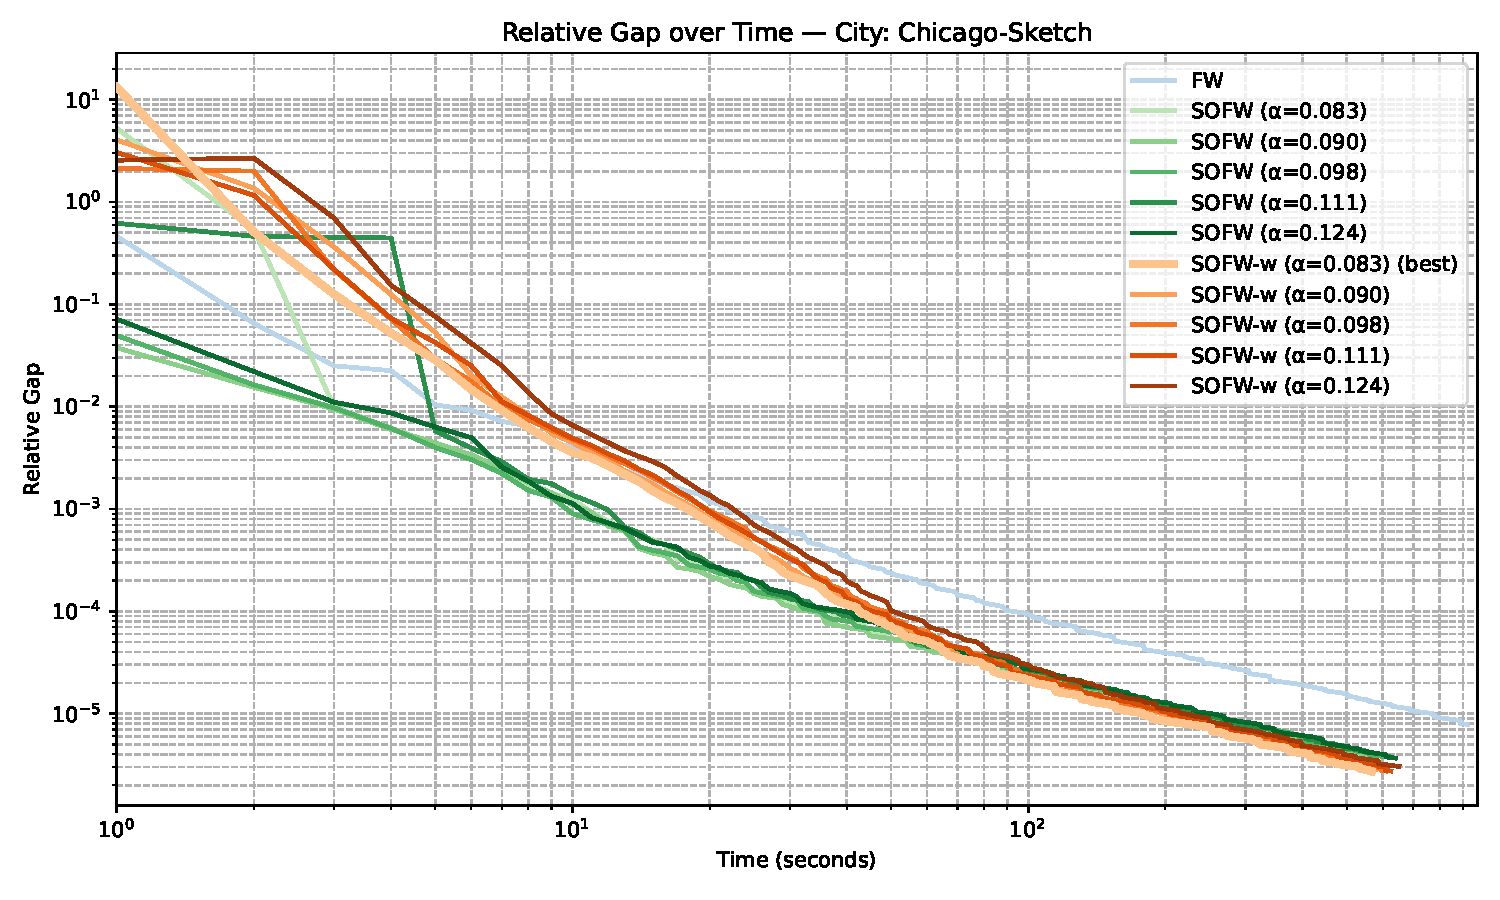
\includegraphics[width=0.48\textwidth]{scfw/Chicago-Sketch.pdf}}
    \subfloat[Birmingham-England]{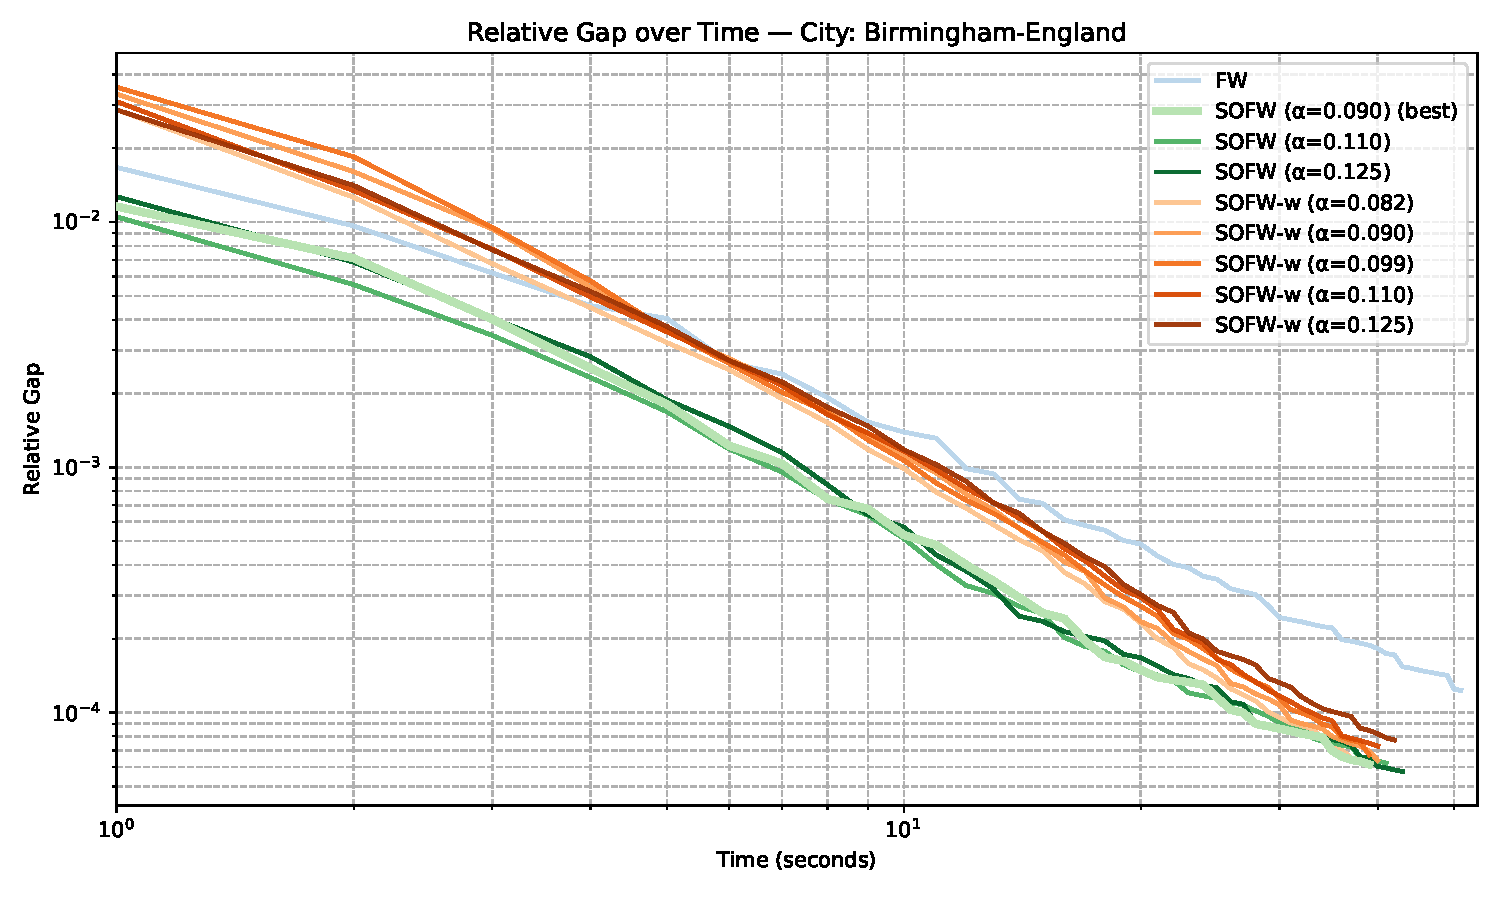
\includegraphics[width=0.48\textwidth]{scfw/Birmingham-England.pdf}}
    \caption{Сравнение SOFW и FW на средних транспортных сетях.}
    \label{fig:sofw-medium-1}
\end{figure}

\begin{figure}[H]
    \centering
    \subfloat[Chicago-Regional]{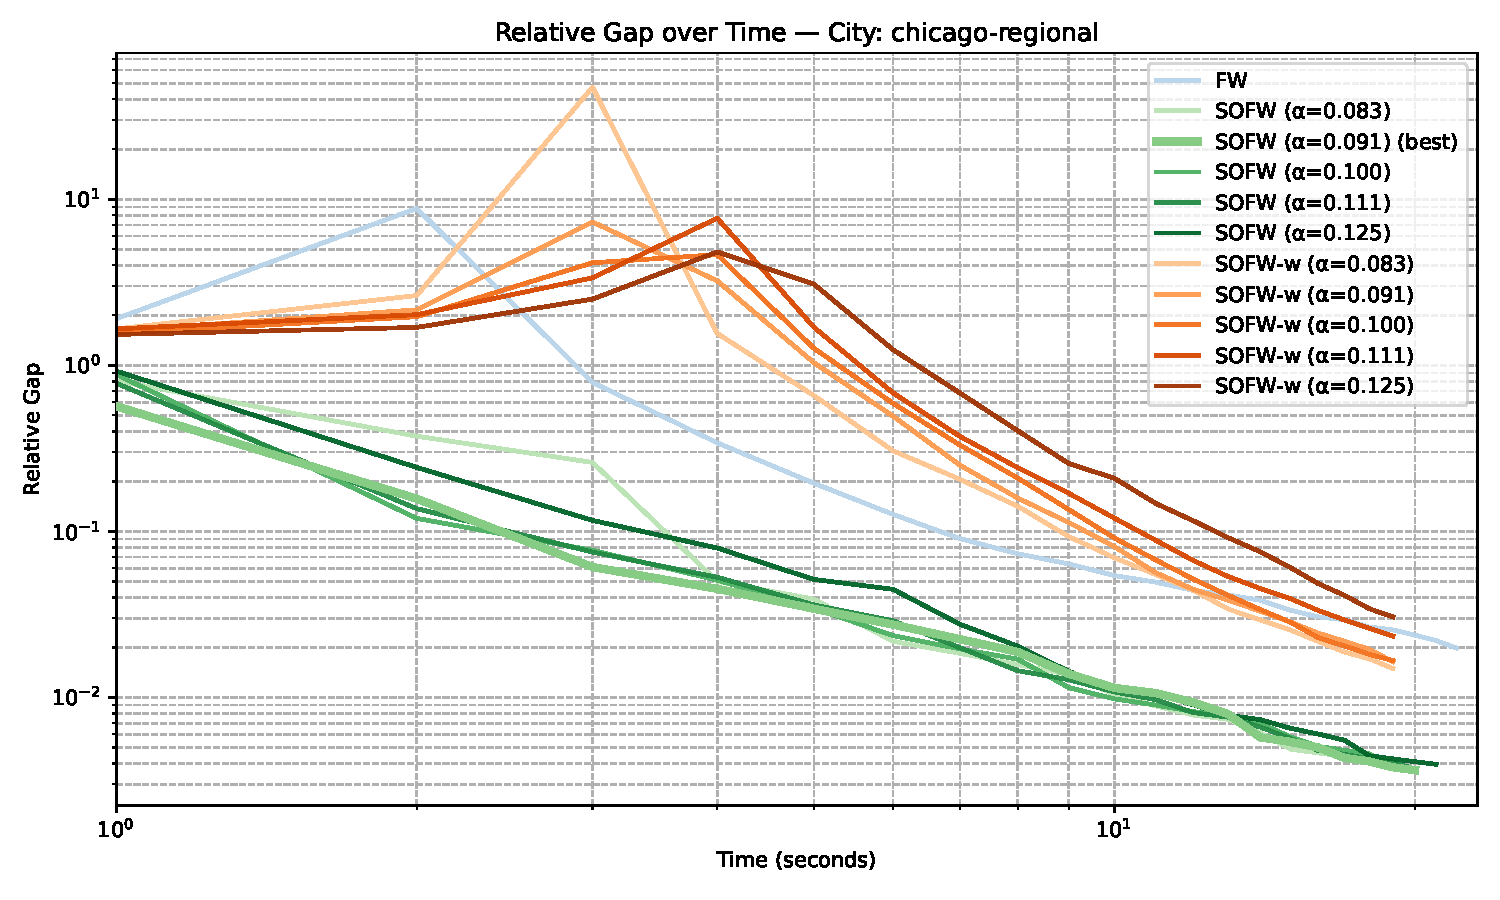
\includegraphics[width=0.48\textwidth]{scfw/chicago-regional.pdf}}
    \subfloat[GoldCoast]{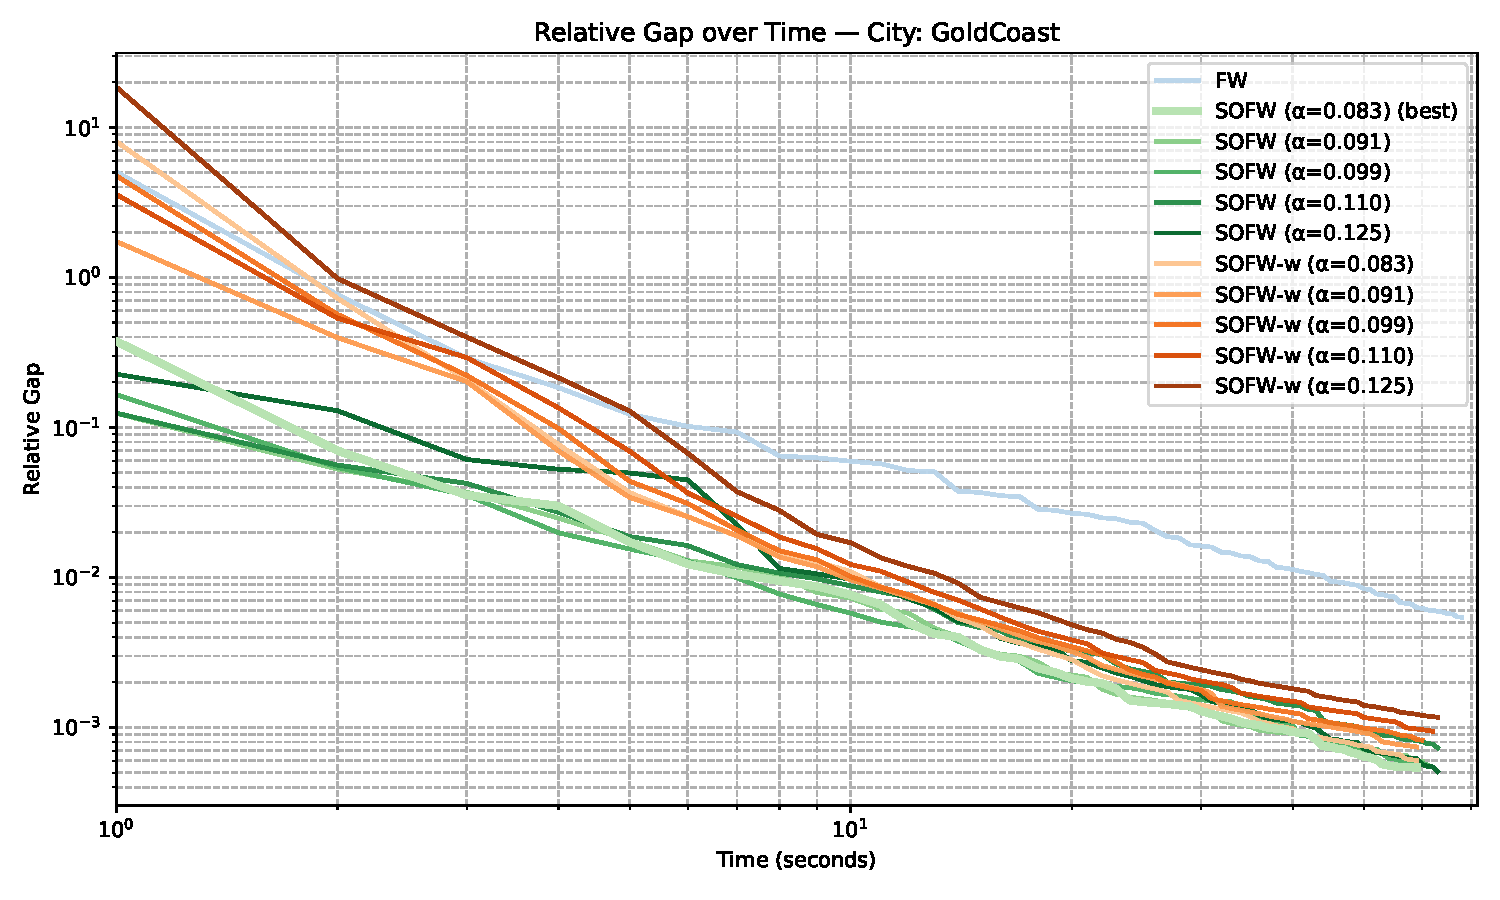
\includegraphics[width=0.48\textwidth]{scfw/GoldCoast.pdf}}
    \caption{SOFW на крупных сетях: выигрыш увеличивается вместе с размером графа.}
    \label{fig:sofw-medium-2}
\end{figure}

\begin{figure}[H]
    \centering
    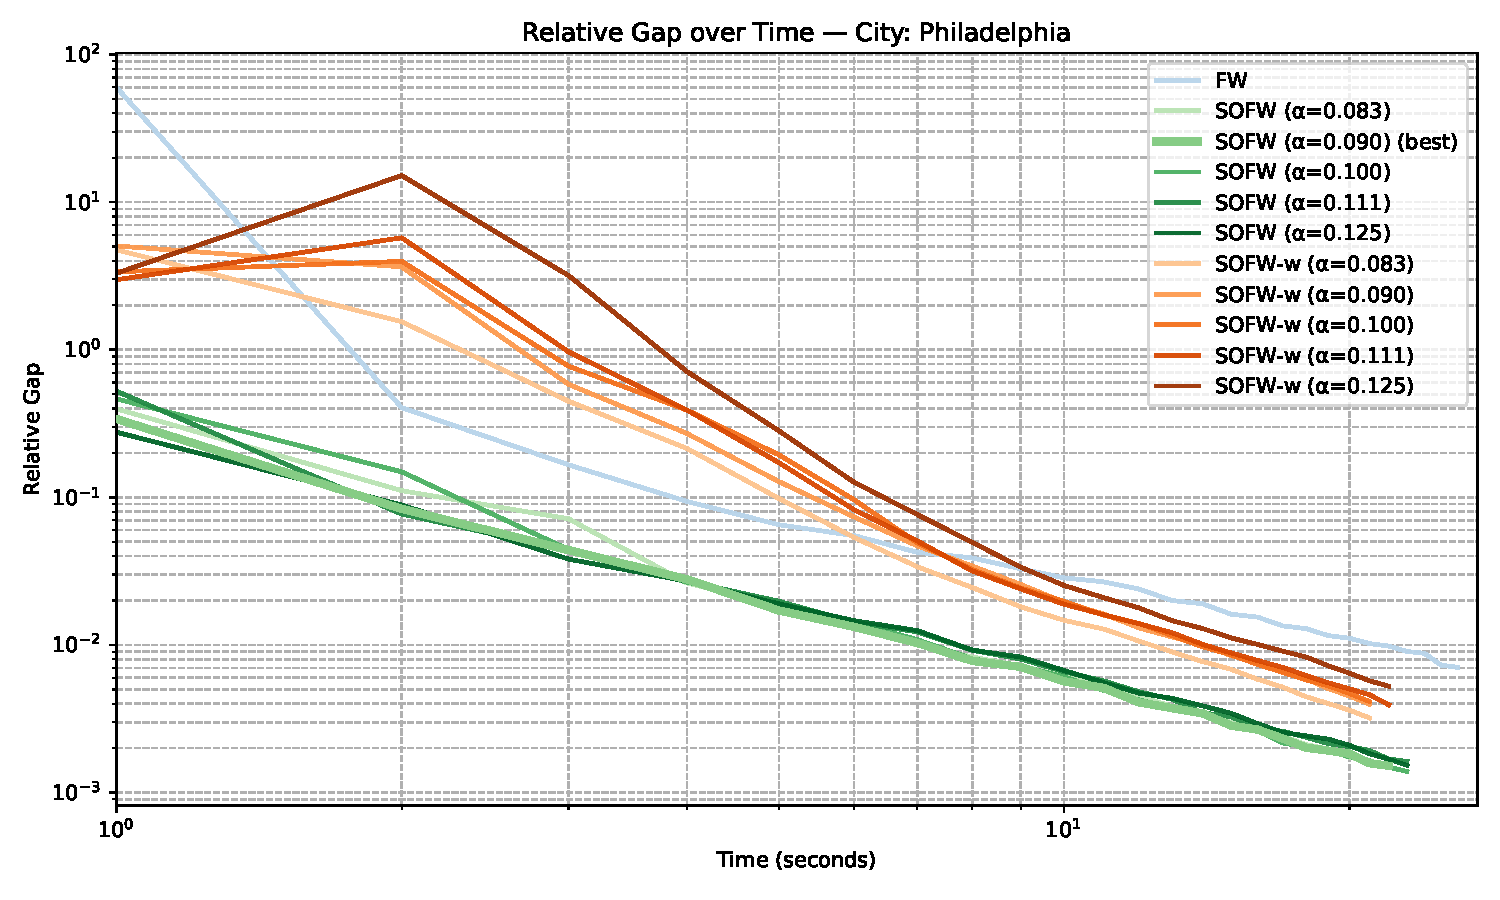
\includegraphics[width=0.8\textwidth]{scfw/Philadelphia.pdf}
    \caption{Датасет Philadelphia: сравнение SOFW и FW на крупной транспортной сети.}
    \label{fig:sofw-philadelphia}
\end{figure}

\begin{figure}[H]
    \centering
    \subfloat[SiouxFalls]{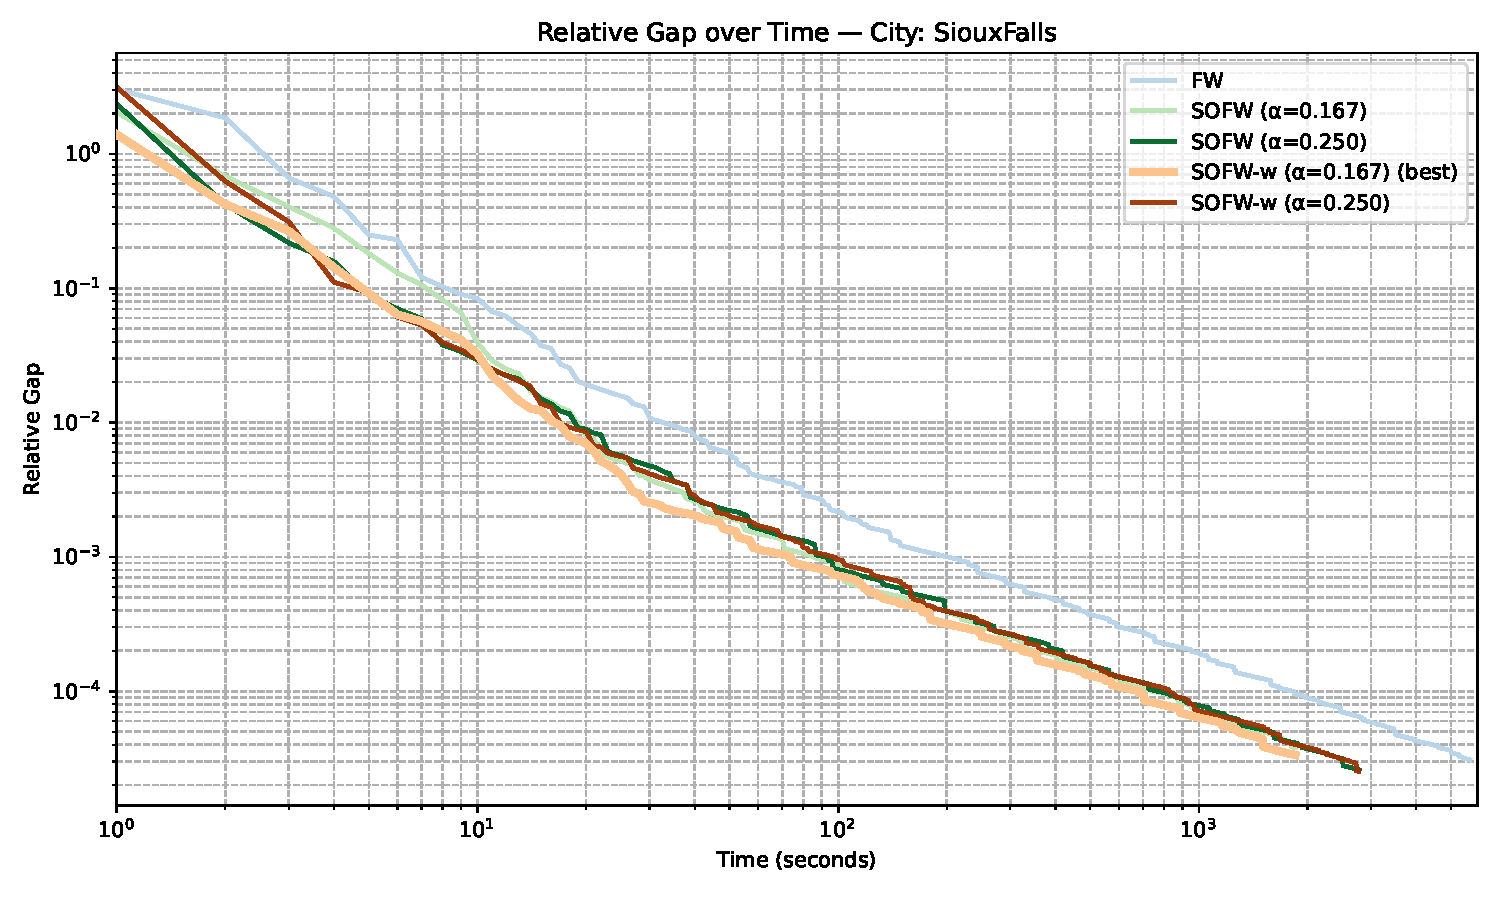
\includegraphics[width=0.48\textwidth]{scfw/SiouxFalls.pdf}}
    \subfloat[Anaheim]{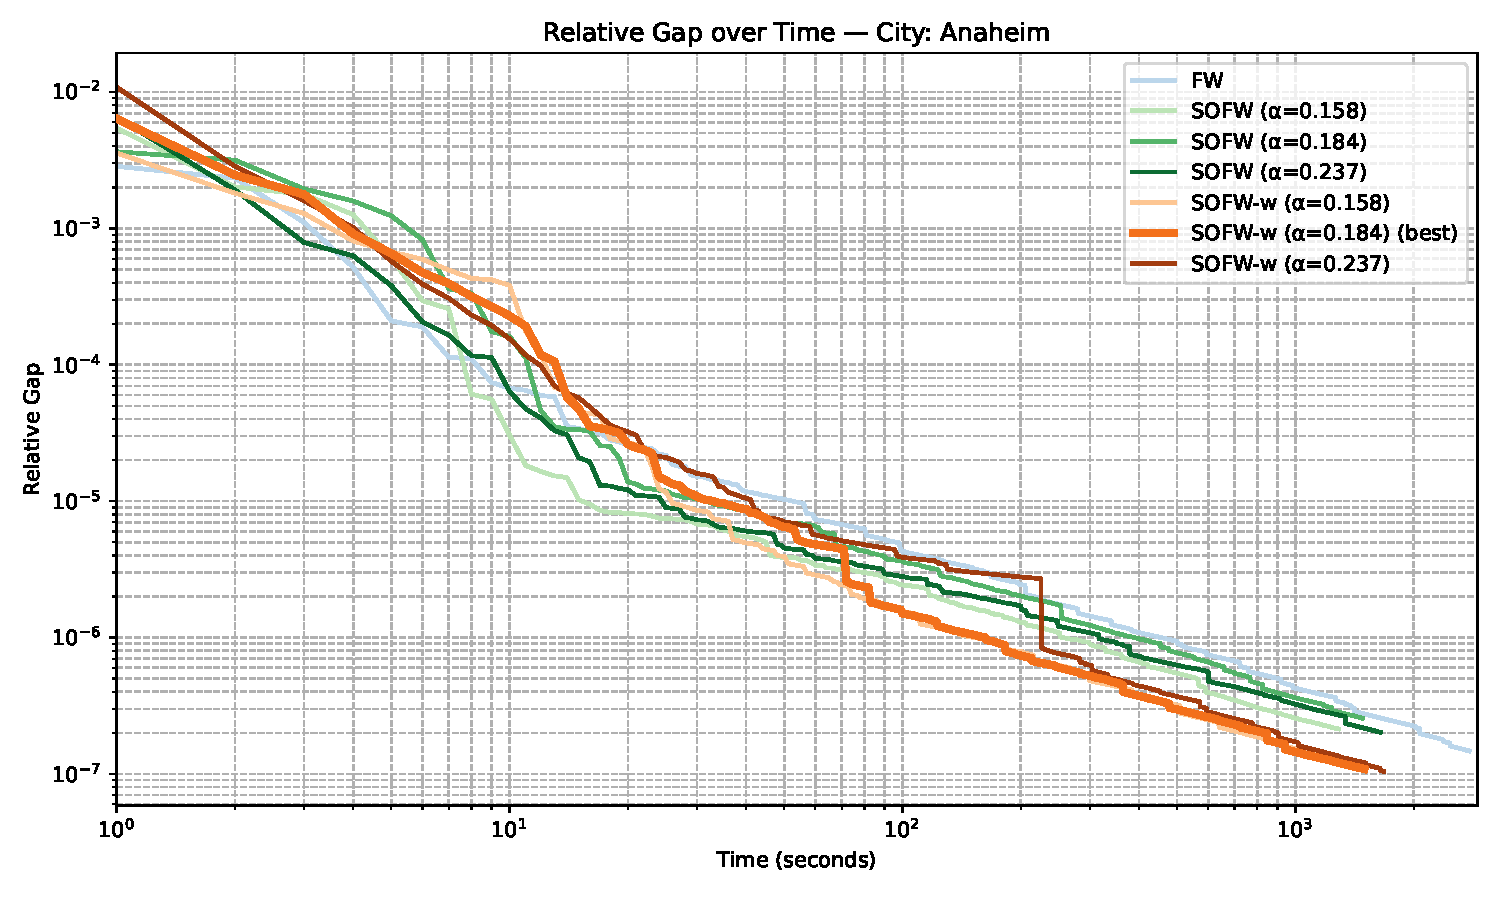
\includegraphics[width=0.48\textwidth]{scfw/Anaheim.pdf}}
    \caption{SOFW и FW на малых сетях: преимущество стохастического подхода менее выражено из-за накладных расходов.}
    \label{fig:sofw-small}
\end{figure}

\begin{figure}[H]
    \centering
    \subfloat[Terrassa-Asymmetric]{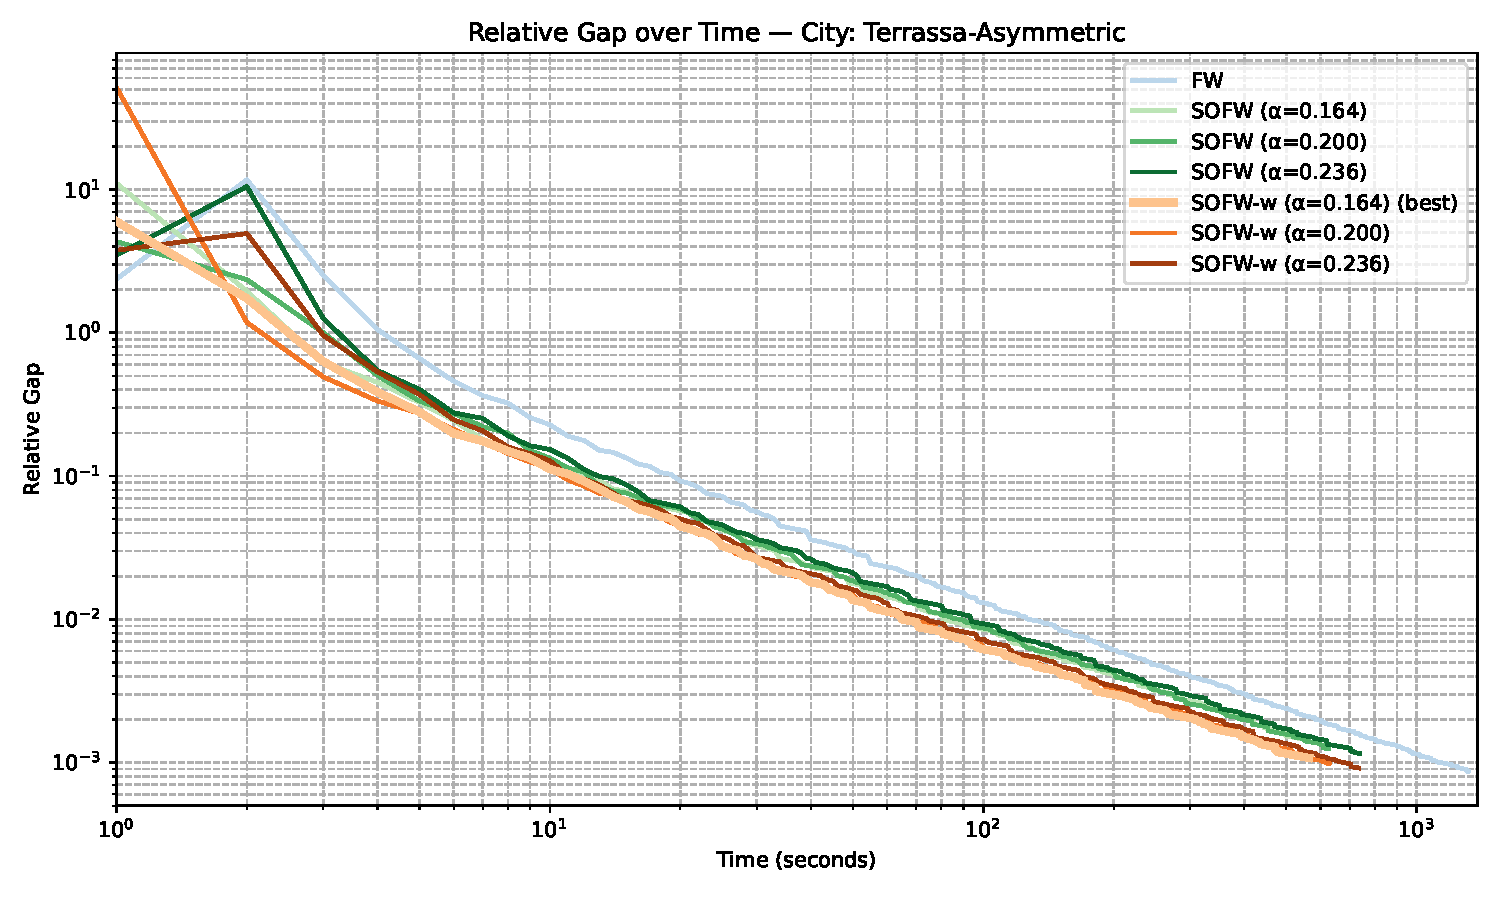
\includegraphics[width=0.48\textwidth]{scfw/Terrassa-Asymmetric.pdf}}
    \subfloat[Winnipeg]{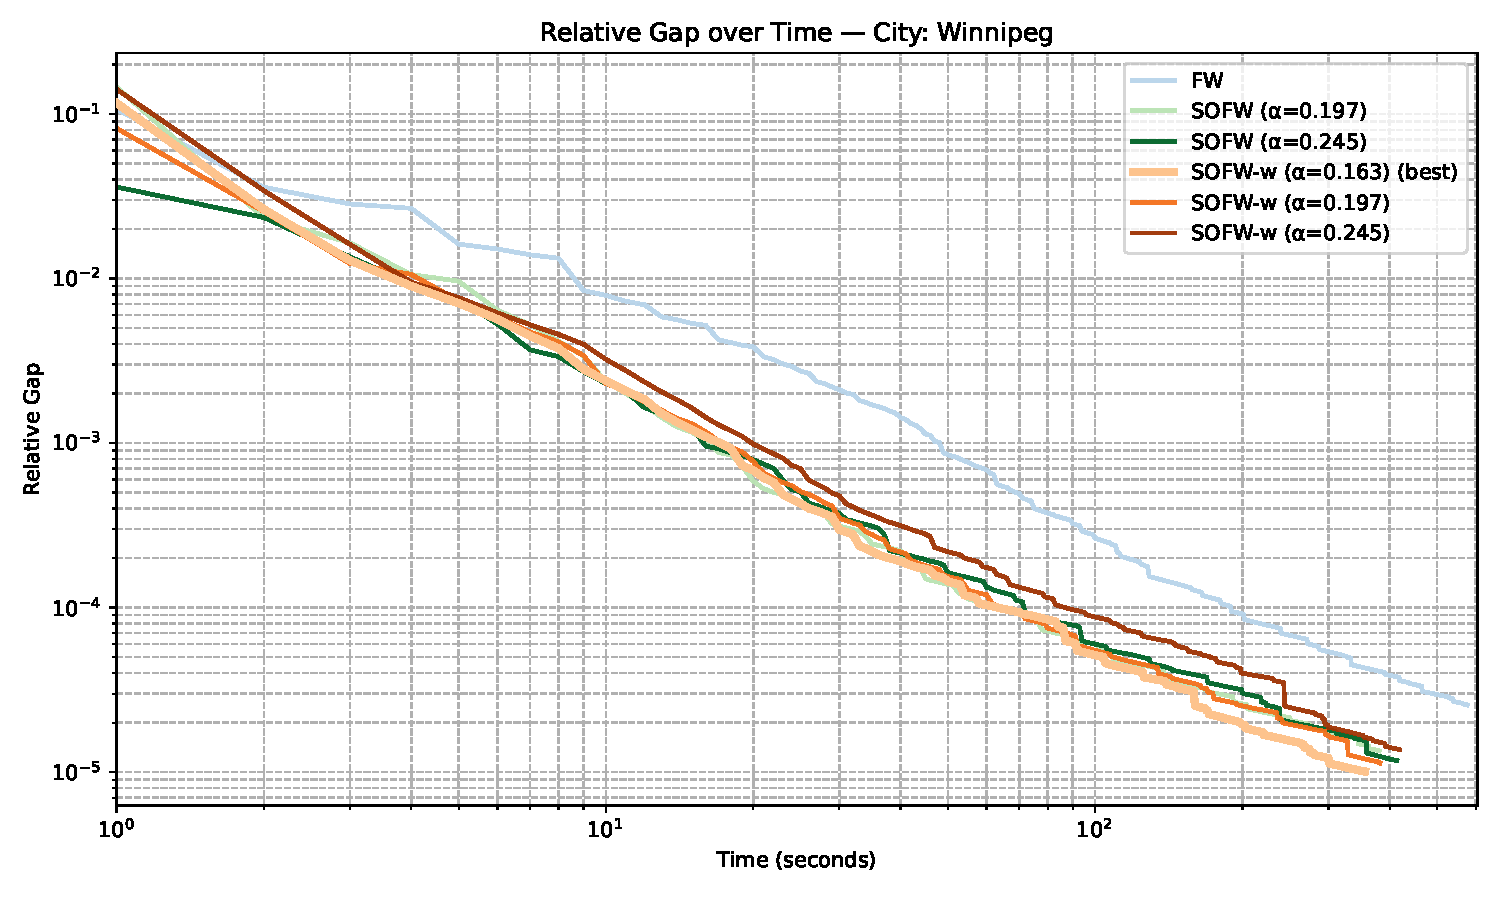
\includegraphics[width=0.48\textwidth]{scfw/Winnipeg.pdf}}
    \caption{Переходная зона между малыми и средними сетями: стохастический подход начинает давать устойчивый выигрыш.}
    \label{fig:sofw-small-2}
\end{figure}

\subsection{Интерпретация графиков SOFW}

На малых сетях SiouxFalls и Anaheim стоимость полного запуска кратчайших путей невелика.
Поэтому экономия от частичного оракула не всегда перекрывает дополнительные расходы:
нужно хранить разложение потока по источникам и аккуратно обновлять только выбранные
компоненты.
На таких задачах классический FW остается сильным базовым методом.

На Terrassa-Asymmetric и Winnipeg картина меняется.
Число зон и ребер уже достаточно велико, чтобы стоимость полной итерации стала заметной.
SOFW начинает выигрывать по времени, особенно на начальном участке, где даже грубое
стохастическое направление быстро снижает зазор.

На Chicago-Sketch, GoldCoast, Birmingham-England, Chicago-Regional и Philadelphia преимущество
становится основным практическим результатом.
Чем больше сеть, тем менее рационально на каждой итерации решать линейный оракул по всем
источникам.
Случайное обновление части источников дает больше итераций за тот же бюджет времени.
Даже если каждая отдельная итерация менее точна, суммарный прогресс оказывается лучше.

Взвешенный вариант SOFW-w особенно полезен на ранних итерациях.
Если источник создает большой суммарный спрос, его вклад в поток по ребрам велик.
Обновление такого источника сильнее меняет функцию Бекмана и быстрее уменьшает грубую
начальную ошибку.
По мере приближения к равновесию различие между равномерным и взвешенным выбором уменьшается:
локальные корректировки становятся тоньше, а роль случайности и конкретных OD-пар возрастает.

Основные экспериментальные выводы:
\begin{enumerate}
    \item SOFW существенно превосходит FW на крупных графах.
    \item Преимущество SOFW растет вместе с размером сети.
    \item На малых сетях метод остается конкурентоспособным, но накладные расходы хранения разложения потока уменьшают выигрыш.
    \item Взвешенный SOFW-w быстрее уменьшает зазор на первых итерациях.
    \item Долгосрочно равномерный и взвешенный варианты дают близкое качество, особенно на крупных графах.
\end{enumerate}

\subsection{Переход от OD-пар к источникам}

Теоретически блоком может быть отдельная OD-пара $w=(i,j)$.
Однако в дорожном графе эффективнее выбирать источники.
Если выбран источник $i$, то один запуск алгоритма кратчайших путей из $i$ дает расстояния
до всех стоков $j$.
Поэтому батч источников
\[
    \mathcal A_k\subset O
\]
порождает батч OD-пар
\[
    \cI_k=\{(i,j)\in OD\mid i\in\mathcal A_k\}.
\]
Такой выбор лучше соответствует структуре вычислений:
стоимость одной итерации примерно пропорциональна числу выбранных источников, а не числу
отдельных OD-пар.

\subsection{Обновление разложения потока}

Пусть
\[
    f_k=\sum_{i\in O}f_k^{(i)}.
\]
Для выбранного источника $i$ строится новый all-or-nothing поток $\hat f_k^{(i)}$:
весь спрос из $i$ назначается на кратчайшие пути при текущих временах $\tau(f_k)$.
Затем направление для этого источника равно
\[
    d_k^{(i)}=\hat f_k^{(i)}-f_k^{(i)}.
\]
Если выбран батч $\mathcal A_k$, суммарное направление записывается как
\[
    d_k=\sum_{i\in\mathcal A_k}d_k^{(i)}.
\]
Обновление выполняется только для выбранных источников:
\[
    f_{k+1}^{(i)}
    =
    \begin{cases}
        f_k^{(i)}+\gamma_k d_k^{(i)}, & i\in\mathcal A_k,\\
        f_k^{(i)}, & i\notin\mathcal A_k.
    \end{cases}
\]
После этого
\[
    f_{k+1}=\sum_{i\in O}f_{k+1}^{(i)}.
\]
Эта формула показывает, почему SOFW требует хранения $f^{(i)}$.
Без такого разложения нельзя локально заменить вклад выбранного источника, не пересчитывая
полный поток.

\subsection{Равномерная и взвешенная выборка}

При равномерной выборке каждый источник имеет одинаковую вероятность попасть в батч.
Это просто и дает чистую теоретическую оценку.
Но спрос по источникам может быть сильно неравномерным.
Если источник генерирует большой поток, его обновление может сильнее уменьшить функционал.
Поэтому рассматривается взвешенная версия.

Пусть
\[
    D_i=\sum_j d_{ij}
\]
-- полный спрос из источника $i$.
Вероятность выбора источника задается как
\[
    p_i=\frac{D_i}{\sum_{\ell\in O}D_\ell}.
\]
Чтобы направление не стало смещенным в сторону крупных источников, можно использовать
importance weighting.
В простейшей записи вклад выбранного источника корректируется множителем $1/p_i$:
\[
    \tilde d_k^{(i)}=\frac{1}{p_i}d_k^{(i)}.
\]
Тогда
\[
    \E[\tilde d_k^{(i)}]=\sum_{i\in O}d_k^{(i)}
\]
с точностью до нормировки батча.
На практике эта коррекция стабилизирует сравнение равномерного и взвешенного SOFW.

\subsection{Влияние батча на теоретический порядок}

Интуитивно может показаться, что батч размера $m$ должен ускорять сходимость в $m$ раз.
Однако в нормированной записи направление усредняется по выбранным блокам.
Ожидаемый прогресс на одну итерацию остается пропорционален полному FW-зазору, деленному
на число блоков:
\[
    \E[\Delta_k\mid x_k]\approx -\frac{\gamma_k}{|OD|}g(x_k).
\]
Батч уменьшает дисперсию, но не меняет этот множитель в базовой оценке.
Практический выигрыш появляется через время выполнения:
если батч можно обработать значительно быстрее полного оракула, то за тот же бюджет времени
алгоритм делает больше обновлений.

\subsection{Память и время}

Если в графе $|O|$ источников и $|\cE|$ ребер, хранение полного потока требует
\[
    \cO(|\cE|)
\]
памяти.
Хранение разложения по источникам требует
\[
    \cO(|O||\cE|)
\]
в худшем случае.
На практике потоки могут быть разреженными, но порядок показывает потенциальную цену SOFW.
Время одной полной итерации FW можно оценить как
\[
    |O|\cdot T_{\mathrm{SP}},
\]
где $T_{\mathrm{SP}}$ -- стоимость одного запуска кратчайших путей.
Если SOFW выбирает долю $\alpha$ источников, то итерация стоит примерно
\[
    \alpha |O|\cdot T_{\mathrm{SP}},
\]
но требует поддерживать разложение $f=\sum_i f^{(i)}$.

\subsection{Итоги раздела}

Стохастический блочно-координатный подход показывает, что для крупных транспортных сетей главная стоимость FW -- это
не формула шага и не вычисление градиента, а полный линейный оракул.
SOFW уменьшает эту стоимость, выбирая только часть источников.
Теоретическая оценка остается такой же по порядку, как у блочного FW, а практические графики
показывают, что на больших сетях экономия времени важнее шума стохастического направления.


\subsection{Выводы по BCFW/SOFW}

Стохастический блочно-координатный подход переносит идею SGD на Frank--Wolfe: вместо полного дорогого оракула используется случайный частичный оракул.
В транспортной задаче такой выбор особенно естественен, поскольку линейная подзадача распадается по источникам и OD-парам.
BCFW/SOFW позволяет масштабировать проекционно-свободную оптимизацию на крупные сети, но требует аккуратного учета компромисса между памятью, числом обновляемых блоков и качеством направления.
Эта же блочная идея используется в следующей главе для построения децентрализованного алгоритма.

\newpage

\section{Децентрализованный блочно-координатный Frank--Wolfe}
\label{sec:dbcfw}

В этой главе рассматривается Decentralized Block-Coordinate Frank--Wolfe (DBCFW).
Это распределенное обобщение блочно-координатного Frank--Wolfe.
Метод опирается на идеи BCFW и децентрализованного FW~\cite{lacoste2013block,wai2017decentralized,vedernikov2023decentralized}.
Метод объединяет три идеи:
\begin{enumerate}
    \item децентрализованный консенсус между вычислительными узлами;
    \item отслеживание градиента для приближения среднего градиента глобальной функции;
    \item стохастический выбор блоков и суженный линейный оракул на каждом узле.
\end{enumerate}
Такой алгоритм естественно продолжает BCFW/SOFW: если в транспортной задаче блоками являются OD-пары или источники, то в общей распределенной постановке блоками являются компоненты декартова произведения допустимого множества.

\subsection{Мотивация и место DBCFW среди FW-методов}

Классический Frank--Wolfe хорошо подходит для задач с простым линейным оракулом и дорогой
проекцией.
Однако в современных задачах машинного обучения часто появляются еще две сложности.
Во-первых, данные распределены между несколькими узлами и не могут быть собраны в одном месте.
Во-вторых, само допустимое множество имеет блочную структуру, поэтому полный линейный оракул
избыточен на каждой итерации.

Decentralized Frank--Wolfe решает первую проблему: каждый агент работает со своей локальной
функцией $f_i$, а согласование происходит через коммуникационный граф.
Block-Coordinate Frank--Wolfe решает вторую проблему: на итерации обновляется только часть
блоков допустимого множества.
DBCFW объединяет эти две идеи.
В результате каждый агент не только использует локальную информацию и общается с соседями,
но и решает линейный оракул только на выбранных блоках.

Такая постановка особенно естественна для задач вида
\[
    D=D_1\times\dots\times D_n,
\]
где каждый блок $D_k$ имеет собственный дешевый линейный оракул.
Если полный оракул по $D$ стоит примерно как сумма оракулов по всем блокам, то обновление
батча размера $B\ll n$ уменьшает стоимость итерации примерно в $n/B$ раз.
Цена этого выигрыша состоит в более шумном направлении и необходимости учитывать ошибки
консенсуса между агентами.

\subsection{Связанные направления}

DBCFW опирается на три линии работ.
Первая линия -- децентрализованный FW с градиентным отслеживанием.
В таких методах каждый агент хранит локальную точку $x_t^i$ и локальную оценку глобального
градиента.
Смешивание точек отвечает за консенсус, а смешивание градиентных оценок отвечает за то,
чтобы каждый агент двигался приблизительно по направлению среднего градиента.

Вторая линия -- блочно-координатный FW.
В BCFW допустимое множество является декартовым произведением, и линейный оракул вызывается
только для случайного блока.
Для выпуклых гладких задач это сохраняет порядок $O(1/t)$ по ожидаемой субоптимальности,
но уменьшает стоимость одной итерации.

Третья линия -- стохастический транспортный FW из предыдущей главы.
SOFW показывает, что блочная случайность может быть не только теоретической конструкцией,
но и практическим способом ускорить задачу транспортного назначения.
DBCFW переносит эту идею на более общую распределенную постановку.

\subsection{Постановка распределенной задачи}

Пусть имеется $N$ узлов.
Узел $i$ имеет доступ только к локальной функции $f_i:D\to\R$.
Требуется решить задачу
\begin{equation}
    \min_{x\in D}
    f(x)
    :=
    \frac{1}{N}\sum_{i=1}^{N}f_i(x),
    \label{eq:dbcfw-problem}
\end{equation}
где $D\subset\R^d$ компактно и выпукло.
Предполагается, что множество имеет блочную структуру
\[
    D=D_1\times\dots\times D_n.
\]
Каждый узел поддерживает локальную точку $x_t^i\in D$.
Средняя точка сети равна
\[
    x_{\mathrm{avg},t}
    =
    \frac{1}{N}\sum_{i=1}^{N}x_t^i.
\]
Диаметр допустимого множества обозначается
\[
    \bar\rho=
    \max_{x,y\in D}\norm{x-y}_2.
\]

\subsection{Коммуникационная модель}

На итерации $t$ узлы обмениваются информацией по графу коммуникаций с матрицей смешивания $W_t\in\R^{N\times N}$.
Граф может меняться от итерации к итерации.
Более того, $W_t$ может быть случайной матрицей, если топология коммуникаций или выбор ребер задаются случайным механизмом.
Используются стандартные предположения из децентрализованной оптимизации~\cite{wai2017decentralized,vedernikov2023decentralized}.

\begin{assumption}
\label{ass:dbcfw-mixing}
Для каждой итерации $t$ матрица $W_t$ согласована с текущим графом коммуникаций:
\[
    (W_t)_{ij}=0,
    \qquad
    i\neq j,\quad (i,j)\notin E_t.
\]
Она неотрицательна и дважды стохастична:
\[
    (W_t)_{ij}\geq0,
    \qquad
    W_t\mathbf{1}=\mathbf{1},
    \qquad
    \mathbf{1}^TW_t=\mathbf{1}^T.
\]
Кроме того, существует $\lambda\in(0,1)$ такая, что для всех $z\in\R^N$
\[
    \left\|
    \left(
        W_t-\frac{1}{N}\mathbf{1}\mathbf{1}^T
    \right)z
    \right\|_2
    \leq
    \lambda\norm{z}_2.
\]
Если графы случайны, все эти свойства предполагаются выполненными почти наверное
условно относительно истории до коммуникационного шага.
Иными словами, далее используется одна и та же константа сжатия $\lambda$ для любой
реализации time-varying последовательности матриц $\{W_t\}$.
\end{assumption}

\begin{assumption}
\label{ass:dbcfw-smooth}
Каждая функция $f_i$ выпукла и $L$-гладка на $D$:
\[
    0
    \leq
    f_i(y)-f_i(x)-\inner{\nabla f_i(x)}{y-x}
    \leq
    \frac{L}{2}\norm{y-x}_2^2,
    \qquad
    x,y\in D.
\]
\end{assumption}

Оценки на ошибки консенсуса и градиентного отслеживания в этой главе не постулируются
отдельно.
Они выводятся ниже из предположений о смешивании, гладкости и компактности множества $D$.

\subsection{Алгоритм DBCFW}

В DBCFW каждый узел сначала смешивает локальные точки с соседями:
\[
    \tilde x_t^i=
    \sum_{j=1}^{N}(W_t)_{ij}x_t^j.
\]
Затем он обновляет локальную оценку градиента и снова применяет смешивание:
\[
    g_t^i=
    \tilde g_{t-1}^i
    +
    \nabla f_i(\tilde x_t^i)
    -
    \nabla f_i(\tilde x_{t-1}^i),
\]
\[
    \tilde g_t^i=
    \sum_{j=1}^{N}(W_t)_{ij}g_t^j.
\]
После этого узел выбирает подмножество блоков $I_t^i\subset\{1,\dots,n\}$ размера $B$ и строит суженное множество:
\[
    D_t^i
    =
    \left(\prod_{k\in I_t^i}D_k\right)
    \times
    \left(\prod_{k\notin I_t^i}\{\tilde x_t^i[k]\}\right).
\]
Линейный оракул решается только на выбранных блоках:
\[
    v_t^i
    \in
    \argmin_{v\in D_t^i}
    \inner{\tilde g_t^i}{v}.
\]
Затем выполняется FW-обновление
\[
    x_{t+1}^i
    =
    (1-\gamma_t)\tilde x_t^i+\gamma_t v_t^i.
\]

\begin{algorithm}
\caption{Decentralized Block-Coordinate Frank--Wolfe}
\label{alg:dbcfw}
\begin{algorithmic}
\REQUIRE множество $D=D_1\times\dots\times D_n$, шаги $\gamma_t$, матрицы $W_t$, размер батча $B$
\STATE инициализировать $x_0^i\in D$, $\tilde x_{-1}^i\gets x_0^i$, $\tilde g_{-1}^i\gets\nabla f_i(\tilde x_{-1}^i)$ для всех $i$
\FOR{$t=0,1,2,\ldots$}
\FORALL{$i\in\{1,\ldots,N\}$ параллельно}
\STATE $\tilde x_t^i\gets\sum_{j=1}^{N}(W_t)_{ij}x_t^j$
\STATE $g_t^i\gets\tilde g_{t-1}^i+\nabla f_i(\tilde x_t^i)-\nabla f_i(\tilde x_{t-1}^i)$
\STATE $\tilde g_t^i\gets\sum_{j=1}^{N}(W_t)_{ij}g_t^j$
\STATE выбрать блоки $I_t^i\subset\{1,\ldots,n\}$, $|I_t^i|=B$
\STATE построить $D_t^i=\left(\prod_{k\in I_t^i}D_k\right)\times\left(\prod_{k\notin I_t^i}\{\tilde x_t^i[k]\}\right)$
\STATE $v_t^i\gets\argmin_{v\in D_t^i}\inner{\tilde g_t^i}{v}$
\STATE $x_{t+1}^i\gets(1-\gamma_t)\tilde x_t^i+\gamma_t v_t^i$
\ENDFOR
\ENDFOR
\end{algorithmic}
\end{algorithm}

\subsection{Связь с классическим DFW}

Если каждый узел на каждой итерации выбирает все блоки,
\[
    I_t^i=\{1,\ldots,n\},
\]
то суженное множество совпадает с исходным:
\[
    D_t^i=D.
\]
В этом случае DBCFW превращается в стандартный Decentralized Frank--Wolfe с градиентным отслеживанием:
\[
    v_t^i\in\argmin_{v\in D}\inner{\tilde g_t^i}{v}.
\]
Следовательно, DBCFW является строгим обобщением децентрализованного FW: он сохраняет консенсус и отслеживание градиента, но заменяет полный линейный оракул блочно-суженным оракулом.

\begin{proposition}
\label{prop:dbcfw-to-dfw}
Если для всех узлов $i$ и всех итераций $t$ выбрано $I_t^i=\{1,\ldots,n\}$,
то алгоритм DBCFW совпадает с децентрализованным Frank--Wolfe с градиентным
отслеживанием.
\end{proposition}

\begin{proof}
При полном выборе блоков имеем
\[
    D_t^i
    =
    \left(\prod_{k=1}^{n}D_k\right)=D.
\]
Следовательно, строка линейного оракула в алгоритме DBCFW принимает вид
\[
    v_t^i
    \in
    \argmin_{v\in D}\inner{\tilde g_t^i}{v}.
\]
Все остальные строки алгоритма не зависят от размера батча:
смешивание точек
\[
    \tilde x_t^i=\sum_{j=1}^{N}(W_t)_{ij}x_t^j
\]
и градиентное отслеживание
\[
    g_t^i=
    \tilde g_{t-1}^i+
    \nabla f_i(\tilde x_t^i)-
    \nabla f_i(\tilde x_{t-1}^i)
\]
остаются теми же.
Значит, единственное отличие DBCFW от DFW исчезает, и полученная схема совпадает с
полным децентрализованным FW.
\end{proof}

\subsection{Полный DFW как предельный случай}

Для ясности запишем соответствующую полную схему.
Каждый агент сначала усредняет точки с соседями, затем обновляет оценку градиента,
после чего решает полный линейный оракул.

\begin{algorithm}
\caption{Decentralized Frank--Wolfe с градиентным отслеживанием}
\label{alg:dfw-full}
\begin{algorithmic}
\REQUIRE множество $D$, шаги $\gamma_t$, матрицы смешивания $W_t$
\STATE инициализировать $x_0^i\in D$ и $g_0^i=\nabla f_i(x_0^i)$
\FOR{$t=0,1,2,\ldots$}
\FORALL{$i=1,\ldots,N$ параллельно}
\STATE $\tilde x_t^i\gets\sum_{j=1}^{N}(W_t)_{ij}x_t^j$
\STATE $\tilde g_t^i\gets\sum_{j=1}^{N}(W_t)_{ij}g_t^j$
\STATE $v_t^i\gets\argmin_{v\in D}\inner{\tilde g_t^i}{v}$
\STATE $x_{t+1}^i\gets(1-\gamma_t)\tilde x_t^i+\gamma_tv_t^i$
\STATE $g_{t+1}^i\gets \tilde g_t^i+\nabla f_i(x_{t+1}^i)-\nabla f_i(x_t^i)$
\ENDFOR
\ENDFOR
\end{algorithmic}
\end{algorithm}

DBCFW заменяет только строку полного оракула.
Вместо $D$ используется $D_t^i$, где невыбранные блоки зафиксированы в точке
$\tilde x_t^i$.
Поэтому DBCFW можно рассматривать как DFW с активным подмножеством координат.

\subsection{Связь с SOFW}

SOFW из главы~\ref{sec:scfw} можно рассматривать как активный блочный FW, где агентами являются OD-пары.
Пусть
\[
    x=(x^w)_{w\in OD},
    \qquad
    \cX=\prod_{w\in OD}\cX^w.
\]
Если на итерации выбрано множество активных корреспонденций $\cI_k\subset OD$, то допустимое множество принимает вид
\[
    \cX_k=
    \left(\prod_{w\in\cI_k}\cX^w\right)
    \times
    \left(\prod_{w\notin\cI_k}\{x_k^w\}\right).
\]
Это полностью совпадает с конструкцией $D_t^i$ в DBCFW, если блоки $D_k$ отождествить с блоками $\cX^w$.
Таким образом,
\[
    \text{агент}
    \longleftrightarrow
    \text{OD-пара},
    \qquad
    \text{активные агенты}
    \longleftrightarrow
    \cI_k,
\]
а локальный оракул агента $w$ имеет вид
\[
    \argmin_{u^w\in\cX^w}
    \inner{\tau(f_k)}{\Theta_wu^w}.
\]
В транспортной задаче этот оракул является поиском кратчайшего пути для выбранной корреспонденции.

\subsection{Отличие SOFW от обычного DFW}

Несмотря на похожую блочную форму, SOFW и DFW имеют разную информационную структуру.
В DFW каждый агент хранит свою копию полного вектора $x$ и пытается согласовать ее с копиями
других агентов.
Случайность, если она есть, обычно связана с коммуникациями или стохастическими градиентами.
В SOFW же нет нескольких копий полного решения.
Есть один глобальный поток, разложенный по источникам или OD-парам, а случайность возникает
из выбора активных блоков.

Это различие важно для алгоритмической интерпретации.
SOFW можно записать как распределенный active-set FW:
каждая OD-пара $w$ отвечает за свой блок $\cX^w$, а на итерации активируется только
подмножество таких ``агентов''.
Но эти агенты не решают независимые локальные задачи с собственными функциями $f_i$.
Все они используют один и тот же глобальный градиент
\[
    \tau(f_k)=\nabla\Psi(f_k),
\]
который зависит от суммарного потока по всем ребрам.

DBCFW находится между этими двумя картинами.
Как DFW, он имеет несколько вычислительных узлов с локальными функциями.
Как SOFW, он использует активные блоки допустимого множества.
Поэтому DBCFW можно рассматривать как общий язык, в котором:
\[
    \text{децентрализация}
    \quad\text{и}\quad
    \text{блочная стохастичность}
\]
описаны одновременно.

\subsection{Кривизна и оценка сходимости}

Для анализа вводятся блочные константы кривизны.
Пусть $D=D_1\times\dots\times D_n$.
Для блока $k$ и точки $x\in D$ определим точку $y$:
\[
    y[j]=
    \begin{cases}
        x[k]+\gamma(s[k]-x[k]), & j=k,\\
        x[j], & j\neq k,
    \end{cases}
    \qquad
    \gamma\in[0,1].
\]
Блочная константа кривизны равна
\[
    C_k
    =
    \sup
    \frac{2}{\gamma^2}
    \left[
        f(y)-f(x)-\inner{\nabla f(x)}{y-x}
    \right].
\]
Глобальная константа кривизны
\[
    C
    =
    \sup
    \frac{2}{\gamma^2}
    \left[
        f(x+\gamma(s-x))
        -
        f(x)
        -
        \gamma\inner{\nabla f(x)}{s-x}
    \right]
\]
удовлетворяет
\[
    C\leq\sum_{k=1}^{n}C_k,
    \qquad
    C\leq L\bar\rho^2.
\]

\begin{lemma}[Консенсусная ошибка для time-varying графов]
\label{lem:dbcfw-consensus}
Пусть выполнено предположение~\ref{ass:dbcfw-mixing}.
Пусть $\alpha\in(0,1]$, шаги удовлетворяют
$0\leq\gamma_t\leq \Gamma t^{-\alpha}$, $\gamma_t\leq1$,
$\Gamma\geq 1$, и пусть $t_0$ -- такое целое число, что
\begin{equation}
\label{eq:dbcfw-t0}
    \lambda
    \leq
    \left(\frac{t_0}{t_0+1}\right)^\alpha
    \frac{1}{1+t_0^{-\alpha}}.
\end{equation}
Тогда для любой реализации time-varying последовательности матриц смешивания, удовлетворяющей
предположению~\ref{ass:dbcfw-mixing}, выполнено
\begin{equation}
\label{eq:dbcfw-consensus-bound}
    \Delta_p^t
    :=
    \max_{1\leq i\leq N}\norm{\tilde x_t^i-x_{\mathrm{avg},t}}_2
    \leq
    \frac{C_p}{t^\alpha},
    \qquad
    C_p=t_0^\alpha\Gamma\sqrt N\,\bar\rho .
\end{equation}
Если графы случайны, оценка выполняется почти наверное и, следовательно, также после
взятия математического ожидания.
\end{lemma}

\begin{proof}
Доказательство ведется pathwise: фиксируем произвольную реализацию последовательности
$\{W_t\}$, для которой выполнено предположение~\ref{ass:dbcfw-mixing}.
Это важно для time-varying случая: в доказательстве используется не фиксированная матрица,
а только равномерное сжатие с одним и тем же $\lambda$ на каждой итерации.

Введем матрицы отклонений
\[
    E_t=
    \begin{bmatrix}
        (x_t^1-x_{\mathrm{avg},t})^T\\
        \vdots\\
        (x_t^N-x_{\mathrm{avg},t})^T
    \end{bmatrix},
    \qquad
    \tilde E_t=
    \begin{bmatrix}
        (\tilde x_t^1-x_{\mathrm{avg},t})^T\\
        \vdots\\
        (\tilde x_t^N-x_{\mathrm{avg},t})^T
    \end{bmatrix}.
\]
Двойная стохастичность $W_t$ сохраняет среднее:
\[
    \frac1N\sum_{i=1}^N\tilde x_t^i=x_{\mathrm{avg},t}.
\]
Поэтому, применяя предположение~\ref{ass:dbcfw-mixing} покоординатно и затем суммируя по
координатам, получаем фробениусово сжатие
\begin{equation}
\label{eq:dbcfw-matrix-contraction}
    \norm{\tilde E_t}_F
    =
    \left\|
        \left(W_t-\frac1N\mathbf 1\mathbf 1^T\right)E_t
    \right\|_F
    \leq
    \lambda\norm{E_t}_F .
\end{equation}
Это равенство не требует постоянного графа: на итерации $t$ используется именно текущая
матрица $W_t$.

Для $1\leq t\leq t_0$ имеем $\tilde x_t^i,x_{\mathrm{avg},t}\in D$: смешанные точки
остаются в $D$ по неотрицательности строк $W_t$ и выпуклости $D$, а средняя точка
также лежит в $D$.
Поэтому
\[
    \norm{\tilde E_t}_F\leq \sqrt N\,\bar\rho
    \leq
    \frac{C_p}{t^\alpha}.
\]
Предположим теперь, что для некоторого $t\geq t_0$ выполнено
$\norm{\tilde E_t}_F\leq C_p/t^\alpha$.
Из FW-обновления
\[
    x_{t+1}^i=(1-\gamma_t)\tilde x_t^i+\gamma_t v_t^i,
    \qquad
    x_{\mathrm{avg},t+1}=(1-\gamma_t)x_{\mathrm{avg},t}
    +\gamma_t v_{\mathrm{avg},t},
\]
где $v_{\mathrm{avg},t}=N^{-1}\sum_i v_t^i$, следует
\[
    x_{t+1}^i-x_{\mathrm{avg},t+1}
    =
    (1-\gamma_t)(\tilde x_t^i-x_{\mathrm{avg},t})
    +
    \gamma_t(v_t^i-v_{\mathrm{avg},t}).
\]
Так как $v_t^i\in D$, $v_{\mathrm{avg},t}\in D$ по выпуклости $D$, и диаметр $D$
равен $\bar\rho$,
\[
    \norm{E_{t+1}}_F
    \leq
    (1-\gamma_t)\norm{\tilde E_t}_F
    +
    \gamma_t\sqrt N\,\bar\rho
    \leq
    \frac{C_p+\Gamma\sqrt N\,\bar\rho}{t^\alpha}.
\]
Применяя сжатие уже с матрицей следующей коммуникации $W_{t+1}$, получаем
\[
    \norm{\tilde E_{t+1}}_F
    \leq
    \lambda
    \frac{C_p+\Gamma\sqrt N\,\bar\rho}{t^\alpha}
    =
    \lambda(1+t_0^{-\alpha})\frac{C_p}{t^\alpha}.
\]
Условие~\eqref{eq:dbcfw-t0} замыкает индукцию:
\[
    \lambda(1+t_0^{-\alpha})\frac{1}{t^\alpha}
    \leq
    \frac{1}{(t+1)^\alpha}.
\]
Следовательно,
\[
    \norm{\tilde E_{t+1}}_F\leq \frac{C_p}{(t+1)^\alpha}.
\]
Поскольку максимум по агентам не превосходит фробениусову норму, получаем
оценку~\eqref{eq:dbcfw-consensus-bound}.
\end{proof}

\begin{lemma}[Ошибка градиентного отслеживания]
\label{lem:dbcfw-gradient-tracking}
Пусть выполнены предположения~\ref{ass:dbcfw-mixing}--\ref{ass:dbcfw-smooth}, а шаги
удовлетворяют условиям леммы~\ref{lem:dbcfw-consensus}.
Обозначим
\[
    \tilde g_t=\frac1N\sum_{i=1}^N\tilde g_t^i.
\]
Тогда для любой реализации time-varying последовательности матриц смешивания выполнено
\begin{equation}
\label{eq:dbcfw-gt-bound}
    \Delta_d^t
    :=
    \max_{1\leq i\leq N}\norm{\tilde g_t^i-\tilde g_t}_2
    \leq
    \frac{C_g}{t^\alpha},
\end{equation}
где $C_g$ можно взять любой константой, удовлетворяющей
\[
    C_g
    \geq
    \max
    \left\{
        t_0^\alpha
        \max_{1\leq s\leq t_0}
        \left(
            \sum_{i=1}^N\norm{\tilde g_s^i-\tilde g_s}_2^2
        \right)^{1/2},
        \;
        2\sqrt N\,t_0^\alpha(2C_p+\Gamma\bar\rho)L
    \right\}.
\]
Если графы случайны, оценка снова имеет pathwise-смысл и потому выполняется почти наверное.
\end{lemma}

\begin{proof}
Как и в лемме~\ref{lem:dbcfw-consensus}, фиксируем произвольную реализацию матриц
$\{W_t\}$.
Сначала заметим, что среднее значение градиентного трекера телескопически совпадает со
средним локальным градиентом в смешанных точках:
\begin{equation}
\label{eq:dbcfw-tracker-average}
    \tilde g_t
    =
    \frac1N\sum_{i=1}^N\nabla f_i(\tilde x_t^i).
\end{equation}
Действительно, двойная стохастичность дает
$N^{-1}\sum_i\tilde g_t^i=N^{-1}\sum_i g_t^i$, а обновление
\[
    g_t^i=
    \tilde g_{t-1}^i+
    \nabla f_i(\tilde x_t^i)-\nabla f_i(\tilde x_{t-1}^i)
\]
после суммирования по $i$ дает телескопическую рекурсию.
Начальное условие алгоритма задает эту рекурсию корректно.

Введем энергию рассогласования
\[
    S_t=
    \left(
        \sum_{i=1}^N\norm{\tilde g_t^i-\tilde g_t}_2^2
    \right)^{1/2}.
\]
Достаточно доказать $S_t\leq C_g/t^\alpha$.
Для конечного числа начальных итераций $1\leq t\leq t_0$ это следует из определения
$C_g$; соответствующий максимум конечен, поскольку $D$ компактно, а градиенты $f_i$
непрерывны на $D$.

Пусть $t\geq t_0$ и $S_t\leq C_g/t^\alpha$.
Обозначим
\[
    \delta_{t+1}^i
    =
    \nabla f_i(\tilde x_{t+1}^i)-\nabla f_i(\tilde x_t^i),
    \qquad
    \bar\delta_{t+1}
    =
    \frac1N\sum_{i=1}^N\delta_{t+1}^i .
\]
Тогда
\[
    g_{t+1}^i=\tilde g_t^i+\delta_{t+1}^i,
    \qquad
    \tilde g_{t+1}^i=\sum_{j=1}^N(W_{t+1})_{ij}g_{t+1}^j,
\]
и, по двойной стохастичности $W_{t+1}$,
$\tilde g_{t+1}=\tilde g_t+\bar\delta_{t+1}$.
Здесь принципиально используется именно $W_{t+1}$: при time-varying графах матрица
следующей коммуникации не обязана совпадать с $W_t$.

Сжатие~\eqref{eq:dbcfw-matrix-contraction}, примененное к векторам $g_{t+1}^i$, дает
\[
    S_{t+1}
    \leq
    \lambda
    \left(
        \sum_{i=1}^N
        \norm{g_{t+1}^i-\tilde g_{t+1}}_2^2
    \right)^{1/2}.
\]
Так как
\[
    g_{t+1}^i-\tilde g_{t+1}
    =
    (\tilde g_t^i-\tilde g_t)+(\delta_{t+1}^i-\bar\delta_{t+1}),
\]
получаем
\begin{equation}
\label{eq:dbcfw-gt-split}
    \left(
        \sum_{i=1}^N
        \norm{g_{t+1}^i-\tilde g_{t+1}}_2^2
    \right)^{1/2}
    \leq
    S_t+
    \left(
        \sum_{i=1}^N
        \norm{\delta_{t+1}^i-\bar\delta_{t+1}}_2^2
    \right)^{1/2}.
\end{equation}

Оценим второе слагаемое.
Из $L$-гладкости
\[
    \norm{\delta_{t+1}^i}_2
    \leq
    L\norm{\tilde x_{t+1}^i-\tilde x_t^i}_2.
\]
Для time-varying графа
\[
    \tilde x_{t+1}^i
    =
    \sum_{j=1}^N(W_{t+1})_{ij}x_{t+1}^j,
\]
поэтому, используя стохастичность строк $W_{t+1}$,
\[
\begin{aligned}
    \norm{\tilde x_{t+1}^i-\tilde x_t^i}_2
    &\leq
    \sum_{j=1}^N(W_{t+1})_{ij}
    \norm{x_{t+1}^j-\tilde x_t^j}_2
    +
    \sum_{j=1}^N(W_{t+1})_{ij}
    \norm{\tilde x_t^j-\tilde x_t^i}_2                                   \\
    &\leq
    \gamma_t\bar\rho+2\Delta_p^t
    \leq
    \frac{\Gamma\bar\rho+2C_p}{t^\alpha}.
\end{aligned}
\]
Здесь первая сумма контролируется FW-шагом, а вторая -- леммой
о консенсусе~\ref{lem:dbcfw-consensus}.
Следовательно,
\[
    \norm{\delta_{t+1}^i}_2
    \leq
    \frac{(\Gamma\bar\rho+2C_p)L}{t^\alpha}.
\]
Поскольку $\bar\delta_{t+1}$ является средним этих приращений,
\[
    \norm{\delta_{t+1}^i-\bar\delta_{t+1}}_2
    \leq
    2\frac{(\Gamma\bar\rho+2C_p)L}{t^\alpha},
\]
и
\[
    \left(
        \sum_{i=1}^N
        \norm{\delta_{t+1}^i-\bar\delta_{t+1}}_2^2
    \right)^{1/2}
    \leq
    2\sqrt N\frac{(\Gamma\bar\rho+2C_p)L}{t^\alpha}
    \leq
    \frac{C_g}{t_0^\alpha t^\alpha}.
\]
Подставляя это и индукционное предположение в~\eqref{eq:dbcfw-gt-split}, имеем
\[
    S_{t+1}
    \leq
    \lambda
    \left(1+t_0^{-\alpha}\right)
    \frac{C_g}{t^\alpha}.
\]
Условие~\eqref{eq:dbcfw-t0} снова дает
\[
    S_{t+1}\leq\frac{C_g}{(t+1)^\alpha}.
\]
Индукция доказана, а из $\max_i\norm{\tilde g_t^i-\tilde g_t}_2\leq S_t$ следует
оценка~\eqref{eq:dbcfw-gt-bound}.
\end{proof}

\begin{theorem}
\label{thm:dbcfw-rate}
Пусть выполнены предположения~\ref{ass:dbcfw-mixing}--\ref{ass:dbcfw-smooth}.
Пусть число блоков равно $n$, а размер батча удовлетворяет $1\leq B\leq n$,
\[
    \tau=\frac{2n}{B},
    \qquad
    \gamma_t=\frac{2n}{B(t+\tau)}.
\]
Для $\alpha=1$ и $\Gamma=2n/B$ леммы~\ref{lem:dbcfw-consensus}
и~\ref{lem:dbcfw-gradient-tracking} дают
\[
    \Delta_p^t
    =
    \max_{1\leq i\leq N}\norm{\tilde x_t^i-x_{\mathrm{avg},t}}_2
    \leq\frac{C_p}{t},
    \qquad
    \Delta_d^t
    =
    \max_{1\leq i\leq N}\norm{\tilde g_t^i-\tilde g_t}_2
    \leq\frac{C_g}{t}.
\]
Тогда для среднего итерата при $t\geq1$ выполняется оценка
\[
    \E[f(x_{\mathrm{avg},t})-f(x^\ast)]
    \leq
    \frac{\widetilde A_\tau}{t+\tau},
\]
где
\[
    A_\tau=
    3\bar\rho(C_g+LC_p)+\frac{L}{2}\bar\rho^2,
\]
\[
    H_1=\E[f(x_{\mathrm{avg},1})-f(x^\ast)],
    \qquad
    \widetilde A_\tau
    =
    \max
    \left\{
        (\tau+1)H_1,
        \frac{4A_\tau n^2}{B^2}
    \right\}.
\]
\end{theorem}

\subsection{Доказательство оценки DBCFW}

Доказательство теоремы~\ref{thm:dbcfw-rate} можно разбить на три шага.
Первый шаг связывает изменение глобальной функции в средней точке сети с усредненным
направлением агентов.
Из $L$-гладкости имеем
\[
    f(x_{\mathrm{avg},t+1})
    \leq
    f(x_{\mathrm{avg},t})
    +
    \inner{\nabla f(x_{\mathrm{avg},t})}
    {x_{\mathrm{avg},t+1}-x_{\mathrm{avg},t}}
    +
    \frac{L}{2}
    \norm{x_{\mathrm{avg},t+1}-x_{\mathrm{avg},t}}_2^2.
\]
Так как матрицы $W_t$ дважды стохастичны, средняя точка после смешивания равна средней
точке до смешивания:
\[
    \frac{1}{N}\sum_{i=1}^{N}\tilde x_t^i
    =
    \frac{1}{N}\sum_{i=1}^{N}x_t^i
    =
    x_{\mathrm{avg},t}.
\]
После FW-обновления
\[
    x_{t+1}^i=(1-\gamma_t)\tilde x_t^i+\gamma_t v_t^i
\]
получаем
\[
    x_{\mathrm{avg},t+1}
    =
    x_{\mathrm{avg},t}
    +
    \gamma_t
    (v_{\mathrm{avg},t}-x_{\mathrm{avg},t}),
    \qquad
    v_{\mathrm{avg},t}=\frac{1}{N}\sum_{i=1}^{N}v_t^i.
\]
Следовательно,
\[
    f(x_{\mathrm{avg},t+1})
    \leq
    f(x_{\mathrm{avg},t})
    +
    \gamma_t
    \inner{\nabla f(x_{\mathrm{avg},t})}
    {v_{\mathrm{avg},t}-x_{\mathrm{avg},t}}
    +
    \frac{L\gamma_t^2}{2}\bar\rho^2.
\]

Второй шаг оценивает, насколько $v_{\mathrm{avg},t}$ близок к истинному FW-направлению.
Главная техническая трудность состоит в том, что в DBCFW агент $i$ решает не полный
линейный оракул на $D$, а ограниченный оракул на $D_t^i$.
Поэтому нельзя напрямую сравнить $v_t^i$ с произвольной точкой $a\in D$.
Для такого сравнения вводится точка $a_t^i(a)$, в которой выбранные блоки берутся из $a$,
а остальные блоки замораживаются в смешанной точке $\tilde x_t^i$:
\[
    a_t^i(a)\in D_t^i,
    \qquad
    \left(a_t^i(a)\right)[k]
    =
    \begin{cases}
        a[k], & k\in I_t^i,\\
        \tilde x_t^i[k], & k\notin I_t^i.
    \end{cases}
\]
Из оптимальности $v_t^i$ на суженном множестве следует
\[
    \inner{v_t^i}{\tilde g_t^i}
    \leq
    \inner{a_t^i(a)}{\tilde g_t^i},
    \qquad a\in D.
\]
Теперь сравним направление агента с истинным градиентом в средней точке.
Для любого $a\in D$ имеем
\[
\begin{aligned}
    &\inner{v_t^i-x_{\mathrm{avg},t}}{\nabla f(x_{\mathrm{avg},t})}  \\
    &=
    \inner{v_t^i-x_{\mathrm{avg},t}}{\tilde g_t^i}
    +
    \inner{v_t^i-x_{\mathrm{avg},t}}
    {\nabla f(x_{\mathrm{avg},t})-\tilde g_t^i}  \\
    &\leq
    \inner{a_t^i(a)-x_{\mathrm{avg},t}}{\tilde g_t^i}
    +
    \norm{v_t^i-x_{\mathrm{avg},t}}_2
    \norm{\nabla f(x_{\mathrm{avg},t})-\tilde g_t^i}_2  \\
    &\leq
    \inner{a_t^i(a)-x_{\mathrm{avg},t}}{\nabla f(x_{\mathrm{avg},t})}
    +
    2\bar\rho
    \norm{\nabla f(x_{\mathrm{avg},t})-\tilde g_t^i}_2.
\end{aligned}
\]
В последнем переходе используется компактность $D$:
$\norm{v_t^i-x_{\mathrm{avg},t}}_2\leq\bar\rho$ и
$\norm{a_t^i(a)-x_{\mathrm{avg},t}}_2\leq\bar\rho$.

Осталось оценить рассогласование градиентов.
Обозначим среднее значение переменных трекинга через
\[
    \tilde g_t=\frac{1}{N}\sum_{i=1}^{N}\tilde g_t^i.
\]
Двойная стохастичность $W_t$ и телескопическая форма градиентного трекинга дают тождество
\[
    \tilde g_t
    =
    \frac{1}{N}\sum_{i=1}^{N}\nabla f_i(\tilde x_t^i).
\]
Поэтому
\[
\begin{aligned}
    \norm{\nabla f(x_{\mathrm{avg},t})-\tilde g_t^i}_2
    &\leq
    \norm{\nabla f(x_{\mathrm{avg},t})-\tilde g_t}_2
    +
    \norm{\tilde g_t-\tilde g_t^i}_2                                      \\
    &\leq
    \frac{1}{N}\sum_{j=1}^{N}
    \norm{\nabla f_j(x_{\mathrm{avg},t})-\nabla f_j(\tilde x_t^j)}_2
    +
    \Delta_d^t                                                            \\
    &\leq
    L\Delta_p^t+\Delta_d^t.
\end{aligned}
\]
Следовательно, для любого $a\in D$
\[
    \inner{v_t^i-x_{\mathrm{avg},t}}{\nabla f(x_{\mathrm{avg},t})}
    \leq
    \inner{a_t^i(a)-x_{\mathrm{avg},t}}{\nabla f(x_{\mathrm{avg},t})}
    +
    2\bar\rho(\Delta_d^t+L\Delta_p^t).
\]

Третий шаг использует блочную случайность.
Пусть $\mathcal F_t$ -- история до выбора блоков на итерации $t$.
Если $I_t^i$ выбирается равномерно без возвращения и $|I_t^i|=B$, то для любого
фиксированного $a\in D$ и любого вектора $w$ выполняется
\[
    \E\left[
        \inner{a_t^i(a)-x_{\mathrm{avg},t}}{w}
        \;\middle|\;\mathcal F_t
    \right]
    =
    \frac{B}{n}\inner{a-x_{\mathrm{avg},t}}{w}
    +
    \left(1-\frac{B}{n}\right)
    \inner{\tilde x_t^i-x_{\mathrm{avg},t}}{w}.
\]
Усреднение по агентам зануляет второй член, поскольку
$N^{-1}\sum_i\tilde x_t^i=x_{\mathrm{avg},t}$.
Берем $w=\nabla f(x_{\mathrm{avg},t})$ и выбираем
\[
    a=s_t\in
    \argmin_{s\in D}
    \inner{\nabla f(x_{\mathrm{avg},t})}{s}.
\]
Тогда из выпуклости
\[
    \inner{s_t-x_{\mathrm{avg},t}}{\nabla f(x_{\mathrm{avg},t})}
    \leq
    -\left(f(x_{\mathrm{avg},t})-f(x^\ast)\right).
\]
В итоге получаем условную оценку спуска
\[
    \E\left[
    \inner{\nabla f(x_{\mathrm{avg},t})}{v_{\mathrm{avg},t}-x_{\mathrm{avg},t}}
    \;\middle|\; \mathcal F_t\right]
    \leq
    -\frac{B}{n}
    (f(x_{\mathrm{avg},t})-f(x^\ast))
    +
    2\bar\rho(\Delta_d^t+L\Delta_p^t).
\]
После подстановки в гладкостную оценку получается рекурсия
\[
    h_{t+1}
    \leq
    \left(1-\frac{B}{n}\gamma_t\right)h_t
    +
    2\gamma_t\bar\rho(\Delta_d^t+L\Delta_p^t)
    +
    \frac{L}{2}\gamma_t^2\bar\rho^2,
\]
где
\[
    h_t=\E[f(x_{\mathrm{avg},t})-f(x^\ast)].
\]
Используя оценки лемм~\ref{lem:dbcfw-consensus} и~\ref{lem:dbcfw-gradient-tracking},
\[
    \Delta_p^t\leq\frac{C_p}{t},
    \qquad
    \Delta_d^t\leq\frac{C_g}{t},
\]
получаем
\[
    h_{t+1}
    \leq
    \left(1-\frac{B}{n}\gamma_t\right)h_t
    +
    \gamma_t
    \frac{2\bar\rho(C_g+LC_p)}{t}
    +
    \frac{L}{2}\gamma_t^2\bar\rho^2.
\]
При выборе
\[
    \gamma_t=\frac{2n}{B(t+\tau)},
    \qquad
    \tau=\frac{2n}{B},
\]
имеем
\[
    \frac{B}{n}\gamma_t=\frac{2}{t+\tau}.
\]
Кроме того,
\[
    \frac{\gamma_t/t}{\gamma_t^2}
    =
    \frac{B(t+\tau)}{2nt}
    =
    \frac{B}{2n}+\frac{1}{t}
    \leq
    \frac12+1
    =
    \frac32,
\]
где использованы $B\leq n$ и $t\geq1$.
Следовательно, $\gamma_t/t\leq(3/2)\gamma_t^2$ для $t\geq1$.
Значит, предыдущая рекурсия переходит в более удобный вид
\[
    h_{t+1}
    \leq
    \left(1-\frac{B}{n}\gamma_t\right)h_t
    +
    \left[
        3\bar\rho(C_g+LC_p)+\frac{L}{2}\bar\rho^2
    \right]\gamma_t^2.
\]
Обозначая
\[
    A_\tau=
    3\bar\rho(C_g+LC_p)+\frac{L}{2}\bar\rho^2,
\]
и используя $\gamma_t^2=4n^2/[B^2(t+\tau)^2]$, перепишем рекурсию как
\[
    h_{t+1}
    \leq
    \left(1-\frac{2}{t+\tau}\right)h_t
    +
    \frac{4A_\tau n^2}{B^2(t+\tau)^2}.
\]
Докажем индукцией, что
\[
    h_t\leq\frac{\widetilde A_\tau}{t+\tau},
    \qquad
    \widetilde A_\tau
    =
    \max
    \left\{
        (\tau+1)h_1,
        \frac{4A_\tau n^2}{B^2}
    \right\}.
\]
База при $t=1$ следует прямо из определения $\widetilde A_\tau$:
\[
    h_1
    \leq
    \frac{\widetilde A_\tau}{\tau+1}.
\]
Если оценка верна для некоторого $t\geq1$, то
\[
\begin{aligned}
    h_{t+1}
    &\leq
    \left(1-\frac{2}{t+\tau}\right)
    \frac{\widetilde A_\tau}{t+\tau}
    +
    \frac{4A_\tau n^2}{B^2(t+\tau)^2}                                      \\
    &\leq
    \left(1-\frac{2}{t+\tau}\right)
    \frac{\widetilde A_\tau}{t+\tau}
    +
    \frac{\widetilde A_\tau}{(t+\tau)^2}
    =
    \frac{\widetilde A_\tau(t+\tau-1)}{(t+\tau)^2}.
\end{aligned}
\]
Так как
\[
    \frac{t+\tau-1}{(t+\tau)^2}
    \leq
    \frac{1}{t+\tau+1},
\]
получаем
\[
    h_{t+1}\leq\frac{\widetilde A_\tau}{t+\tau+1}.
\]
Индукция замкнута.
Так сохраняется порядок $O(1/t)$, а влияние децентрализации и батчирования переносится
в константу $\widetilde A_\tau$.

Смысл оценки состоит в том, что DBCFW сохраняет порядок $O(1/t)$ для выпуклой гладкой задачи,
а нужное убывание ошибок консенсуса и отслеживания градиента обеспечивается леммами
выше.
Размер батча $B$ влияет на константы: увеличение числа обновляемых блоков делает шаг ближе к полному DFW, но повышает стоимость линейного оракула.

\subsection{Блочный линейный оракул}

Для $D=D_1\times\dots\times D_n$ полный линейный оракул равен
\[
    \argmin_{v\in D}\inner{g}{v}.
\]
Он распадается по блокам:
\[
    v[k]\in\argmin_{u\in D_k}\inner{g[k]}{u}.
\]
DBCFW использует только выбранный набор $I_t^i$:
\[
    v_t^i[k]\in
    \begin{cases}
        \argmin_{u\in D_k}\inner{\tilde g_t^i[k]}{u}, & k\in I_t^i,\\
        \tilde x_t^i[k], & k\notin I_t^i.
    \end{cases}
\]
Таким образом, невыбранные блоки не меняются в направлении оракула.
После FW-шага они также остаются ближе к текущей смешанной точке:
\[
    x_{t+1}^i[k]=\tilde x_t^i[k],
    \qquad k\notin I_t^i,
\]
если записывать $v_t^i[k]=\tilde x_t^i[k]$.

\subsection{Специальные случаи DBCFW}

DBCFW содержит несколько известных схем как частные случаи.
Если $N=1$, то нет децентрализации и коммуникаций.
Алгоритм превращается в стохастический блочно-координатный FW:
\[
    x_{t+1}=(1-\gamma_t)x_t+\gamma_tv_t,
\]
где $v_t$ отличается от $x_t$ только на выбранных блоках.

Если $B=n$, то каждый агент выбирает все блоки.
Алгоритм превращается в DFW с градиентным отслеживанием.

Если одновременно $N=1$ и $B=n$, то DBCFW становится классическим FW.
Именно поэтому DBCFW удобно рассматривать как общий каркас:
\[
    \text{FW}
    \subset
    \text{BCFW}
    \subset
    \text{DBCFW},
    \qquad
    \text{DFW}
    \subset
    \text{DBCFW}.
\]

\subsection{Интерпретация констант в оценке}

В теореме~\ref{thm:dbcfw-rate} константа
\[
    A_\tau=
    3\bar\rho(C_g+LC_p)+\frac{L}{2}\bar\rho^2
\]
содержит два типа ошибок.
Слагаемое
\[
    3\bar\rho(C_g+LC_p)
\]
отвечает за несовпадение локальных направлений с направлением, которое использовал бы
централизованный алгоритм.
Здесь $C_g$ связан с ошибкой градиентного отслеживания, а $LC_p$ возникает из-за того,
что локальные точки отличаются от средней точки.
Слагаемое
\[
    \frac{L}{2}\bar\rho^2
\]
является обычной гладкостной ценой FW-шага.

Параметр
\[
    \tau=\frac{2n}{B}
\]
увеличивается при малом батче.
Если $B$ мал, шаг должен быть осторожнее, потому что один оракул покрывает меньшую часть
координат.
Если $B=n$, то $\tau=2$, и схема ближе к полному DFW.

\subsection{Итоги раздела}

DBCFW формулируется как общий метод для распределенной проекционно-свободной
оптимизации на декартовых множествах.
Главный алгоритмический объект -- локальный блочный линейный оракул, который вызывается
после смешивания точек и градиентного отслеживания.
Главный теоретический результат -- сохранение порядка $O(1/t)$: леммы о консенсусе и
градиентном отслеживании дают нужное убывание ошибок, а теорема использует эти оценки
в рекурсии спуска.
Главная связь с предыдущими главами состоит в том, что стохастический выбор блоков из SOFW
становится частью распределенного FW-каркаса.


\subsection{Выводы по DBCFW}

DBCFW завершает хронологию развития методов в этой работе.
Сначала предыдущие направления использовались для ускорения FW в одной централизованной задаче.
Затем CFW и NFW были перенесены на машинное обучение.
После этого блочная структура позволила стохастически уменьшить стоимость линейного оракула.
DBCFW объединяет блочную экономию вычислений с распределенной архитектурой, где данные и функции разделены между узлами.

Алгоритм особенно полезен в задачах, где:
\begin{enumerate}
    \item допустимое множество имеет декартову блочную структуру;
    \item линейный оракул по полному множеству слишком дорог по сравнению с блочным оракулом;
    \item данные или функции распределены между несколькими агентами;
    \item коммуникации между агентами ограничены сетевым графом.
\end{enumerate}
Таким образом, DBCFW является естественным кандидатом для крупномасштабных распределенных задач машинного обучения и сетевой оптимизации.

\newpage

\section{Заключение}

В работе рассмотрена последовательная линия развития алгоритма Frank--Wolfe для задач машинного обучения и крупномасштабной выпуклой оптимизации.
Сначала были описаны модификации FW, использующие предыдущие направления в задаче равновесного распределения транспортных потоков.
Затем эти идеи были перенесены на задачи машинного обучения, сводимые к гладкой выпуклой оптимизации на компактном множестве.
После этого была рассмотрена стохастическая блочно-координатная версия, уменьшающая стоимость линейного оракула за счет обновления только части блоков.
Наконец, была сформулирована децентрализованная блочно-координатная схема, объединяющая линейные оракулы, консенсус и отслеживание градиента.

Основные результаты работы:
\begin{enumerate}
    \item Описаны CFW, BFW, FFW, WFFW и NFW как модификации FW, ускоряющие сходимость за счет памяти о предыдущих направлениях.
    \item Показано, что CFW можно применять в машинном обучении без явного вычисления гессиана, используя приближение через разности градиентов.
    \item Приведена оценка сходимости CFW по зазору Frank--Wolfe, совпадающая по порядку со стандартной оценкой FW.
    \item Описан SOFW/BCFW как блочно-координатный метод для транспортных сетей, уменьшающий стоимость итерации за счет стохастического выбора источников.
    \item Сформулирован DBCFW.
    Это децентрализованное расширение блочного FW с градиентным отслеживанием.
\end{enumerate}

\subsection{Итоги по главам}

В первой главе было показано, что основная слабость классического FW в транспортной
задаче связана не с линейным оракулом, а с геометрией направления.
CFW, BFW и NFW используют прошлые направления для уменьшения зигзагообразного поведения,
а FFW и WFFW решают похожую задачу через сглаживание.
Экспериментальные результаты показывают, что память о нескольких направлениях
может существенно ускорять уменьшение относительного зазора.

Во второй главе эта идея была перенесена в машинное обучение.
Ключевой технический шаг состоит в отказе от явного гессиана.
Вместо произведения $\nabla^2 f(x_k)d_{k-1}$ используется разность соседних градиентов.
Благодаря этому CFW и NFW становятся применимыми к логистической регрессии с ограничением
на $l_1$-норму.
Эксперименты на Mushrooms и MNIST показывают, что выигрыш особенно заметен, когда
безусловное решение находится далеко от границы допустимого множества.

В третьей главе основное внимание было перенесено с направления на стоимость итерации.
SOFW обновляет только часть источников транспортной сети и тем самым уменьшает стоимость
линейного оракула.
Теоретически метод соответствует блочно-координатному FW и сохраняет стандартный порядок
сходимости в ожидании.
Практически же он выигрывает на крупных сетях, где полный запуск кратчайших путей становится
главной вычислительной нагрузкой.

В четвертой главе блочная идея была соединена с децентрализованной оптимизацией.
DBCFW сохраняет механизм консенсуса и градиентного отслеживания из DFW, но заменяет полный
линейный оракул блочным.
Если выбрать все блоки, метод возвращается к обычному DFW.
Если убрать децентрализацию, получается блочный FW.
Поэтому DBCFW является естественным завершающим звеном рассматриваемой хронологии.

\subsection{Ограничения и дальнейшая работа}

Ограничение рассмотренной линии методов состоит в том, что каждая модификация улучшает
свой вычислительный аспект: направление шага, стоимость линейного оракула или распределенную
архитектуру.
Единый метод, который одновременно использует сопряженные направления, стохастический выбор
блоков и децентрализованный консенсус, остается отдельной исследовательской задачей.
Перспективным направлением является объединение стохастического выбора блоков с сопряженными
направлениями NFW, а также экспериментальная проверка DBCFW на распределенных задачах
машинного обучения.

\newpage

\setcounter{secnumdepth}{0}
\section{Список использованных источников}
\begingroup
\renewcommand{\section}[2]{}
\begin{thebibliography}{99}

\bibitem{frank1956algorithm}
Frank M., Wolfe P. An algorithm for quadratic programming // Naval Research Logistics Quarterly. 1956. Vol. 3. No. 1--2. P. 95--110.

\bibitem{jaggi2013revisiting}
Jaggi M. Revisiting Frank--Wolfe: Projection-Free Sparse Convex Optimization // Proceedings of the 30th International Conference on Machine Learning. 2013. Vol. 28. P. 427--435.

\bibitem{braun2022conditional}
Braun G., Pokutta S., Tu S., Wright S. Blended conditional gradients: the unconditioning of conditional gradients // SIAM Journal on Optimization. 2022.

\bibitem{patriksson2015traffic}
Patriksson M. The Traffic Assignment Problem: Models and Methods. Dover Publications, 2015.

\bibitem{mitradjieva2013stiff}
Mitradjieva M., Lindberg P. O. The Stiff Is Moving: Conjugate Direction Frank--Wolfe Methods with Applications to Traffic Assignment // Transportation Science. 2013. Vol. 47. No. 2. P. 280--293.

\bibitem{fukushima1984modified}
Fukushima M. A modified Frank--Wolfe algorithm for solving the traffic assignment problem // Transportation Research Part B: Methodological. 1984. Vol. 18. No. 2. P. 169--177.

\bibitem{arrache2008accelerating}
Arrache S., Ouafi R. Accelerating Convergence of the Frank--Wolfe Algorithm for Solving the Traffic Assignment Problem // International Journal of Computer Science and Network Security. 2008. Vol. 8. No. 5. P. 181--186.

\bibitem{ignashin2024modifications}
Игнашин И. Н., Ярмошик Д. В. Модификации алгоритма Frank--Wolfe в задаче поиска равновесного распределения транспортных потоков // Компьютерные исследования и моделирование. 2024. Т. 16. No. 1. С. 53--68. DOI: \url{https://doi.org/10.20537/2076-7633-2024-16-1-53-68}.

\bibitem{bstabler}
Stabler B. Transportation Networks for Research Core Team. TransportationNetworks repository. URL: \url{https://github.com/bstabler/TransportationNetworks}.

\bibitem{jaggi2012blockcoordfw}
Jaggi M., Lacoste-Julien S., Schmidt M. Block-Coordinate Frank--Wolfe Optimization for Structural SVMs // Proceedings of the 30th International Conference on Machine Learning. 2013.

\bibitem{lacoste2013block}
Lacoste-Julien S., Jaggi M., Schmidt M., Pletscher P. Block-Coordinate Frank--Wolfe Optimization for Structural SVMs // Proceedings of the 30th International Conference on Machine Learning. 2013. P. 53--61.

\bibitem{ignashin2026stochastic}
Ignashin I., Yarmoshik D., Raigorodskii A. Stochastic Origin Frank--Wolfe Method for Traffic Assignment // Journal of Mathematical Sciences. 2025. Vol. 295. No. 2. P. 170--184. DOI: \url{https://doi.org/10.1007/s10958-025-08157-6}.

\bibitem{wai2017decentralized}
Wai H.-T., Lafond J., Scaglione A., Moulines E. Decentralized Frank--Wolfe Algorithm for Convex and Nonconvex Problems // IEEE Transactions on Automatic Control. 2017. Vol. 62. No. 11. P. 5522--5537.

\bibitem{vedernikov2023decentralized}
Vedernikov R., Rogozin A., Gasnikov A. Decentralized Conditional Gradient Method over Time-Varying Graphs // arXiv preprint arXiv:2307.10978. 2023.

\bibitem{beckmann1956studies}
Beckmann M., McGuire C. B., Winsten C. B. Studies in the Economics of Transportation. Yale University Press, 1956.

\bibitem{wardrop1952road}
Wardrop J. G. Some theoretical aspects of road traffic research // Proceedings of the Institution of Civil Engineers. 1952. Vol. 1. No. 3. P. 325--362.

\bibitem{bpr1964traffic}
Bureau of Public Roads. Traffic Assignment Manual. U.S. Department of Commerce, Urban Planning Division, 1964.

\bibitem{sheffi1985urban}
Sheffi Y. Urban Transportation Networks: Equilibrium Analysis with Mathematical Programming Methods. Prentice-Hall, 1985.

\bibitem{leblanc1985improved}
LeBlanc L. J., Morlok E. K., Pierskalla W. P. An improved method for the solution of the transportation network equilibrium problem // Transportation Science. 1975. Vol. 9. No. 4. P. 309--318.

\bibitem{luenberger1984linear}
Luenberger D. G. Linear and Nonlinear Programming. Addison-Wesley, 1984.

\bibitem{bertsekas1999nonlinear}
Bertsekas D. P. Nonlinear Programming. Athena Scientific, 1999.

\bibitem{nesterov1983method}
Nesterov Y. A method for solving the convex programming problem with convergence rate $O(1/k^2)$ // Soviet Mathematics Doklady. 1983. Vol. 27. No. 2. P. 372--376.

\bibitem{nesterov2018lectures}
Nesterov Y. Lectures on Convex Optimization. Springer, 2018.

\bibitem{pedregosa2020linearly}
Pedregosa F., Negiar G., Askari A., Jaggi M. Linearly convergent Frank--Wolfe with backtracking line-search // Proceedings of the 23rd International Conference on Artificial Intelligence and Statistics. 2020. P. 1--10.

\bibitem{pearlmutter1994fast}
Pearlmutter B. A. Fast exact multiplication by the Hessian // Neural Computation. 1994. Vol. 6. No. 1. P. 147--160.

\bibitem{jax2018github}
Bradbury J., Frostig R., Hawkins P., Johnson M. J., Leary C., Maclaurin D., Wanderman-Milne S. JAX: composable transformations of Python+NumPy programs. 2018. URL: \url{https://github.com/google/jax}.

\bibitem{lecun1998mnist}
LeCun Y., Cortes C., Burges C. The MNIST database of handwritten digits. 1998. URL: \url{http://yann.lecun.com/exdb/mnist/}.

\bibitem{dua2019uci}
Dua D., Graff C. UCI Machine Learning Repository. University of California, Irvine, School of Information and Computer Sciences, 2019.

\bibitem{tibshirani1996regression}
Tibshirani R. Regression shrinkage and selection via the lasso // Journal of the Royal Statistical Society: Series B. 1996. Vol. 58. No. 1. P. 267--288.

\end{thebibliography}
\endgroup
\setcounter{secnumdepth}{3}


\end{document}
